% $Author$
% $Date$
% $Revision$

% HISTORY:
% 2006-10-05 - Oscar started
% 2007-05-28 - Stef edit
% 2007-06-06 - Oscar first draft
% 2007-08-14 - Stef corrections
% 2007-09-06 - Lukas review

%=================================================================
\ifx\wholebook\relax\else
% --------------------------------------------
% Lulu:
	\documentclass[a4paper,10pt,twoside]{book}
	\usepackage[
		papersize={6in,9in},
		hmargin={.75in,.75in},
		vmargin={.75in,1in},
		ignoreheadfoot
	]{geometry}
	% $Author$
% $Date$
% $Revision$

% HISTORY:
% 2006-10-31 - Oscar code macros
% ...

%=============================================================
% NB: documentclass must be set in main document.
% Allows book to be generated in multiple formats.
%=============================================================
%:Packages
\usepackage[T1]{fontenc}  %%%%%% really important to get the code directly in the text!
\usepackage{lmodern}
%\usepackage[scaled=0.85]{bookmanx} % needs another scale factor if used with \renewcommand{\sfdefault}{cmbr}
\usepackage{palatino}
\usepackage[scaled=0.85]{helvet}
\usepackage[protrusion,expansion=false]{microtype}
\usepackage{graphicx}
\usepackage{theorem}
\usepackage[english]{babel}
% ON: pdfsync breaks the use of p{width} for tabular columns!
\ifdefined\usepdfsync\usepackage{pdfsync}\fi % Requires texlive 2007
%=============================================================
%:More packages
%Stef should check which ones are used!
%\usepackage{picinpar}
%\usepackage{layout}
%\usepackage{color}
%\usepackage{enum}
%\usepackage{a4wide}
% \usepackage{fancyhdr}
\usepackage{ifthen}
\usepackage{float}
\usepackage{longtable}
\usepackage{makeidx}
\usepackage[nottoc]{tocbibind}
\usepackage{multicol}
\usepackage{booktabs}	% book-style tables
\usepackage{topcapt}	% enables \topcaption
\usepackage{multirow}
\usepackage{tabularx}
%\usepackage[bottom]{footmisc}
\usepackage{xspace}
\usepackage{alltt}
\usepackage{amssymb,textcomp}
\usepackage[usenames,dvipsnames]{color}
%\usepackage{colortbl}
\usepackage[hang]{subfigure}\makeatletter\def\p@subfigure{\thefigure\,}\makeatother
\usepackage{rotating}
\usepackage{enumitem}	% apb: allows more control over tags in enumerations
\usepackage{verbatim}     % for comment environment
\usepackage{varioref}	% for page references that work
\labelformat{footnote}{\thechapter--#1} % to distinguish citations from jurabib
\usepackage{needspace}
\usepackage{isodateo} % enable \isodate
\usepackage[newparttoc]{titlesec}
\usepackage{titletoc}
\usepackage{wrapfig}
\usepackage[
	super,
	citefull=first,
	authorformat={allreversed,and},
	titleformat={commasep,italic}
]{jurabib} % citations as footnotes
\usepackage[
	colorlinks=true,
	linkcolor=black,
	urlcolor=black,
	citecolor=black
]{hyperref}   % should come last
%=============================================================
%:PDF version
\pdfminorversion=3 % Set PDF to 1.3 for Lulu
%=============================================================
%:URL style
\makeatletter
\def\url@leostyle{%
  \@ifundefined{selectfont}{\def\UrlFont{\sf}}{\def\UrlFont{\sffamily}}}
\makeatother
% Now actually use the newly defined style.
\urlstyle{leo}
%=============================================================
%:Booleans
\newboolean{lulu}
\setboolean{lulu}{false}
\newcommand{\ifluluelse}[2]{\ifthenelse{\boolean{lulu}}{#1}{#2}}
%=============================================================
%:Names
\newcommand{\SUnit}{SUnit\xspace}
\newcommand{\sunit}{SUnit\xspace}
\newcommand{\xUnit}{$x$Unit\xspace}
\newcommand{\JUnit}{JUnit\xspace}
\newcommand{\st}{Smalltalk\xspace}
\newcommand{\pharo}{Pharo\xspace} % Use this, not \Pharo
%\newcommand{\sqmap}{SqueakMap\xspace}
\newcommand{\squeak}{Squeak\xspace} % use this, not \Squeak or \sq
\newcommand{\sqsrc}{SqueakSource\xspace}
\newcommand{\sbe}{\url{http://SqueakByExample.org}\xspace}
\newcommand{\pharoweb}{\url{http://pharo-project.org}\xspace}
\newcommand{\pbe}{\url{http://PharoByExample.org}\xspace}
\newcommand{\sba}{\url{http://SquareBracketAssociates.org}\xspace}
\newcommand{\bam}{\lct{Bounc\-ing\-Atoms\-Morph}\xspace}
%=============================================================
%:Markup macros for proof-reading
\usepackage[normalem]{ulem} % for \sout
\usepackage{xcolor}
\newcommand{\ra}{$\rightarrow$}
\newcommand{\ugh}[1]{\textcolor{red}{\uwave{#1}}} % please rephrase
\newcommand{\ins}[1]{\textcolor{blue}{\uline{#1}}} % please insert
\newcommand{\del}[1]{\textcolor{red}{\sout{#1}}} % please delete
\newcommand{\chg}[2]{\textcolor{red}{\sout{#1}}{\ra}\textcolor{blue}{\uline{#2}}} % please change
%=============================================================
%:Editorial comment macros
%\newcommand{\nnbb}[2]{
%    % \fbox{\bfseries\sffamily\scriptsize#1}
%    \fcolorbox{gray}{yellow}{\bfseries\sffamily\scriptsize#1}
%    {\sf\small$\blacktriangleright$\textit{#2}$\blacktriangleleft$}
%   }
\newcommand{\yellowbox}[1]{\fcolorbox{gray}{yellow}{\bfseries\sffamily\scriptsize#1}}
\newcommand{\triangles}[1]{{\sf\small$\blacktriangleright$\textit{#1}$\blacktriangleleft$}}
\newcommand{\nnbb}[2]{\yellowbox{#1} \triangles{#2}}
\newcommand{\fix}{\yellowbox{FIX!}}
\newcommand{\here}{\yellowbox{CONTINUE HERE!}}
% editor macros
\newcommand{\apl}[1]{\nnbb{Alain}{#1}} % Alain
\newcommand{\ab}[1]{\nnbb{Andrew}{#1}} % Black
\newcommand{\sd}[1]{\nnbb{St\'{e}f}{#1}} % Ducasse
\newcommand{\dc}[1]{\nnbb{DamienC}{#1}} % Ducasse
\newcommand{\md}[1]{\nnbb{Marcus}{#1}} % Denker
\newcommand{\on}[1]{\nnbb{Oscar}{#1}} % Nierstrasz
\newcommand{\damien}[1]{\nnbb{Damien}{#1}} % Pollet
\newcommand{\lr}[1]{\nnbb{Lukas}{#1}} % Renggli
\newcommand{\orla}[1]{\nnbb{Orla}{#1}} % Greevy
\newcommand{\alex}[1]{\nnbb{Alex}{#1}} % Bergel
\newcommand{\alx}[1]{\nnbb{Alex}{#1}} % Bergel
\newcommand{\dr}[1]{\nnbb{David}{#1}} % Roethlisberger
\newcommand{\ja}[1]{\nnbb{Jannik}{#1}} % Laval
\newcommand{\jr}[1]{\nnbb{Jorge}{#1}} % Ressia
\newcommand{\jb}[1]{\nnbb{JB}{#1}} % JB
\newcommand{\fp}[1]{\nnbb{Fabrizio}{#1}} % Perin
\newcommand{\michael}[1]{\nnbb{Michael}{#1}} % Davies
\newcommand{\ew}[1]{\nnbb{Erwann}{#1}} % Wernli
\newcommand{\mb}[1]{\nnbb{Martial}{#1}} % Boniou
\newcommand{\hw}[1]{\nnbb{Hernan}{#1}} % Wilkinson
\newcommand{\ben}[1]{\nnbb{Benjamin}{#1}} % Benjamin Van Ryseghem
%=============================================================
%:Abbreviation macros
\newcommand{\ie}{\emph{i.e.},\xspace}
\newcommand{\eg}{\emph{e.g.},\xspace}
\newcommand{\etc}{etc.\xspace}
%=============================================================
%:Cross reference macros
\newcommand{\charef}[1]{Chapter~\ref{cha:#1}\xspace}
\newcommand{\secref}[1]{Section~\ref{sec:#1}\xspace}
\newcommand{\figref}[1]{Figure~\ref{fig:#1}\xspace}
\newcommand{\Figref}[1]{Figure~\ref{fig:#1}\xspace}
\newcommand{\appref}[1]{Appendix~\ref{app:#1}\xspace}
\newcommand{\tabref}[1]{Table~\ref{tab:#1}\xspace}
\newcommand{\faqref}[1]{FAQ~\ref{faq:#1}, p.~\pageref{faq:#1}\xspace}
% APB: I removed trailing \xspace commands from these macros because
% \xspace mostly doesn't work.  If you want a space after your
% references, type one!
% ON: xspace has always worked just fine for me!  Please leave them in.
%
\newcommand{\ruleref}[1]{\ref{rule:#1}\xspace}
%
\newcommand{\egref}[1]{example~\ref{eg:#1}\xspace}
\newcommand{\Egref}[1]{Example~\ref{eg:#1}\xspace}
%
\newcommand{\scrref}[1]{script~\ref{scr:#1}\xspace}
\newcommand{\Scrref}[1]{Script~\ref{scr:#1}\xspace}
\newcommand{\tscrref}[1]{the script~\ref{scr:#1}\xspace}
\newcommand{\Tscrref}[1]{The script~\ref{scr:#1}\xspace}
%
\newcommand{\mthref}[1]{method~\ref{mth:#1}\xspace}
\newcommand{\mthsref}[1]{methods~\ref{mth:#1}\xspace}
\newcommand{\Mthref}[1]{Method~\ref{mth:#1}\xspace}
\newcommand{\tmthref}[1]{the method~\ref{mth:#1}\xspace}
\newcommand{\Tmthref}[1]{The method~\ref{mth:#1}\xspace}
%
\newcommand{\clsref}[1]{class~\ref{cls:#1}\xspace}
\newcommand{\tclsref}[1]{the class~\ref{cls:#1}\xspace}
\newcommand{\Tclsref}[1]{The class~\ref{cls:#1}\xspace}

\newcommand{\chalabel}[1]{\label{cha:#1}}
\newcommand{\seclabel}[1]{\label{sec:#1}}
\newcommand{\figlabel}[1]{\label{fig:#1}}
\newcommand{\tablabel}[1]{\label{tab:#1}}
\newcommand{\rulelabel}[1]{\label{rule:#1}}
\newcommand{\eglabel}[1]{\label{eg:#1}}
\newcommand{\scrlabel}[1]{\label{scr:#1}}
\newcommand{\mthlabel}[1]{\label{mth:#1}}
\newcommand{\clslabel}[1]{\label{cls:#1}}
\newcommand{\faqlabel}[1]{\label{faq:#1}}
%=============================================================
%:Menu item macro
% for menu items, so we can change our minds on how to print them! (apb)
\definecolor{lightgray}{gray}{0.89}
\newcommand{\menu}[1]{{%
	\setlength{\fboxsep}{0pt}%
	\colorbox{lightgray}{{{\upshape\sffamily\strut \,#1\,}}}}}
\newcommand{\link}[1]{{%
	\fontfamily{lmr}\selectfont
 	\upshape{\sffamily \underline{#1}}}}
% For submenu items:
\newcommand{\go}{\,$\triangleright$\,}
% \newcommand{\go}{\,$\blacktriangleright$\,}
% For keyboard shortcuts:
%\newcommand{\short}[1]{\mbox{$\langle${\sc CMD}$\rangle$-#1}\xspace}
\newcommand{\short}[1]{\mbox{{\sc cmd}\hspace{0.08em}--\hspace{0.09em}#1}\xspace}
% For buttons:
\newcommand{\button}[1]{{%
	\setlength{\fboxsep}{0pt}%
	\fbox{{\upshape\sffamily\strut \,#1\,}}}}
% NB: The button macro does not work within captions -- incompatible with xcolor package :-(
\newcommand{\toolsflap}{\textit{Tools} flap\xspace}
%=============================================================
%:Mouse clicks
\newcommand{\click}{click\xspace} % RED
\newcommand{\actclick}{action-click\xspace} % YELLOW
\newcommand{\metaclick}{meta-click\xspace} % BLUE
\newcommand{\Click}{Click\xspace} % RED
\newcommand{\Actclick}{Action-click\xspace} % YELLOW
\newcommand{\Metaclick}{Meta-click\xspace} % BLUE
%=============================================================
%:ToSh macros
\newboolean{tosh}
\setboolean{tosh}{false}
\newcommand{\iftoshelse}[2]{\ifthenelse{\boolean{tosh}}{#1}{#2}}
%=============================================================
%:ToSh colors
%\newcommand{\highlightcolor}{\color{blue!65}}
%\newcommand{\boxcolor}{\color{gray!25}}
\newcommand{\highlight}[1]{\textcolor{blue!65}{#1}}
%\newcommand{\codecolor}{\color{blue!65}}
%%\setlength{\fboxrule}{2pt}
%\newcommand{\asPict}[1]{%
%	{\Large\highlight{#1}}}
%=============================================================
%:Reader cues (do this)
%
% Indicate something the reader should try out.
% \newcommand{\dothisicon}{\raisebox{-.5ex}{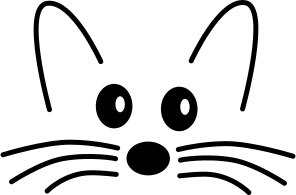
\includegraphics[width=1.4em]{squeak-logo}}}
\iftoshelse{
	\usepackage{marginnote}
		\renewcommand*{\marginfont}{\footnotesize}
	\newcommand{\vartriangleout}{\ifthenelse{\isodd{\thepage}}{\vartriangleright}{\vartriangleleft}}
	\newcommand{\dothisicon}{\fcolorbox{blue!65}{white}{\highlight{$\vartriangleout$}}}
	\newcommand{\dothis}[1]{%
		\noindent\par\noindent
		{\reversemarginpar
			\marginnote{\fcolorbox{blue!65}{white}{\highlight{$\vartriangleout$}}}}
		%\MarginLabel{do this}
		\noindent\emph{#1}
		\nopagebreak}
}{
	\newcommand{\dothisicon}{\raisebox{-.5ex}{
\includegraphics[height=1.2em]{pharo}}}
	\newcommand{\dothis}[1]{%
		\medskip
		\noindent\dothisicon
		\ifx#1\empty\else\quad\emph{#1}\fi
		\par\smallskip\nopagebreak}
}
%===> NEW VERSION <===
% NB: To use this in an individual chapter, you must set:
%\graphicspath{{figures/} {../figures/}}
% at the head of the chapter.  Don't forget the final /
%=============================================================
%:Reader hints (hint)
%
% Indicates a non-obvious consequence 
\newcommand{\hint}[1]{\vspace{1ex}\noindent\fbox{\textsc{Hint}} \emph{#1}}
%=================================================================
% graphics for Morphic handles
\newcommand{\grabHandle}{\raisebox{-0.2ex}{
\includegraphics[width=1em]{blackHandle}}}
\newcommand{\moveHandle}{\raisebox{-0.2ex}{
\includegraphics[width=1em]{moveHandle}}}
\newcommand{\debugHandle}{\raisebox{-0.2ex}{
\includegraphics[width=1em]{debugHandle}}}
%=============================================================
%:Highlighting Important stuff (doublebox)
%
% From Seaside book ...
\newsavebox{\SavedText}
\newlength{\InnerBoxRule}\setlength{\InnerBoxRule}{.75\fboxrule}
\newlength{\OuterBoxRule}\setlength{\OuterBoxRule}{1.5\fboxrule}
\newlength{\BoxSeparation}\setlength{\BoxSeparation}{1.5\fboxrule}
\addtolength{\BoxSeparation}{.5pt}
\newlength{\SaveBoxSep}\setlength{\SaveBoxSep}{2\fboxsep}
%
\newenvironment{doublebox}{\begin{lrbox}{\SavedText}
    \begin{minipage}{.75\textwidth}}
    {\end{minipage}\end{lrbox}\begin{center}
    \setlength{\fboxsep}{\BoxSeparation}\setlength{\fboxrule}{\OuterBoxRule}
    \fbox{\setlength{\fboxsep}{\SaveBoxSep}\setlength{\fboxrule}{\InnerBoxRule}%
      \fbox{\usebox{\SavedText}}}
  \end{center}}
% Use this:
\newcommand{\important}[1]{\begin{doublebox}#1\end{doublebox}}
%=============================================================
%:Section depth
\setcounter{secnumdepth}{2}
%% for this to happen start the file with
%\ifx\wholebook\relax\else
%% $Author$
% $Date$
% $Revision$

% HISTORY:
% 2006-10-31 - Oscar code macros
% ...

%=============================================================
% NB: documentclass must be set in main document.
% Allows book to be generated in multiple formats.
%=============================================================
%:Packages
\usepackage[T1]{fontenc}  %%%%%% really important to get the code directly in the text!
\usepackage{lmodern}
%\usepackage[scaled=0.85]{bookmanx} % needs another scale factor if used with \renewcommand{\sfdefault}{cmbr}
\usepackage{palatino}
\usepackage[scaled=0.85]{helvet}
\usepackage[protrusion,expansion=false]{microtype}
\usepackage{graphicx}
\usepackage{theorem}
\usepackage[english]{babel}
% ON: pdfsync breaks the use of p{width} for tabular columns!
\ifdefined\usepdfsync\usepackage{pdfsync}\fi % Requires texlive 2007
%=============================================================
%:More packages
%Stef should check which ones are used!
%\usepackage{picinpar}
%\usepackage{layout}
%\usepackage{color}
%\usepackage{enum}
%\usepackage{a4wide}
% \usepackage{fancyhdr}
\usepackage{ifthen}
\usepackage{float}
\usepackage{longtable}
\usepackage{makeidx}
\usepackage[nottoc]{tocbibind}
\usepackage{multicol}
\usepackage{booktabs}	% book-style tables
\usepackage{topcapt}	% enables \topcaption
\usepackage{multirow}
\usepackage{tabularx}
%\usepackage[bottom]{footmisc}
\usepackage{xspace}
\usepackage{alltt}
\usepackage{amssymb,textcomp}
\usepackage[usenames,dvipsnames]{color}
%\usepackage{colortbl}
\usepackage[hang]{subfigure}\makeatletter\def\p@subfigure{\thefigure\,}\makeatother
\usepackage{rotating}
\usepackage{enumitem}	% apb: allows more control over tags in enumerations
\usepackage{verbatim}     % for comment environment
\usepackage{varioref}	% for page references that work
\labelformat{footnote}{\thechapter--#1} % to distinguish citations from jurabib
\usepackage{needspace}
\usepackage{isodateo} % enable \isodate
\usepackage[newparttoc]{titlesec}
\usepackage{titletoc}
\usepackage{wrapfig}
\usepackage[
	super,
	citefull=first,
	authorformat={allreversed,and},
	titleformat={commasep,italic}
]{jurabib} % citations as footnotes
\usepackage[
	colorlinks=true,
	linkcolor=black,
	urlcolor=black,
	citecolor=black
]{hyperref}   % should come last
%=============================================================
%:PDF version
\pdfminorversion=3 % Set PDF to 1.3 for Lulu
%=============================================================
%:URL style
\makeatletter
\def\url@leostyle{%
  \@ifundefined{selectfont}{\def\UrlFont{\sf}}{\def\UrlFont{\sffamily}}}
\makeatother
% Now actually use the newly defined style.
\urlstyle{leo}
%=============================================================
%:Booleans
\newboolean{lulu}
\setboolean{lulu}{false}
\newcommand{\ifluluelse}[2]{\ifthenelse{\boolean{lulu}}{#1}{#2}}
%=============================================================
%:Names
\newcommand{\SUnit}{SUnit\xspace}
\newcommand{\sunit}{SUnit\xspace}
\newcommand{\xUnit}{$x$Unit\xspace}
\newcommand{\JUnit}{JUnit\xspace}
\newcommand{\st}{Smalltalk\xspace}
\newcommand{\pharo}{Pharo\xspace} % Use this, not \Pharo
%\newcommand{\sqmap}{SqueakMap\xspace}
\newcommand{\squeak}{Squeak\xspace} % use this, not \Squeak or \sq
\newcommand{\sqsrc}{SqueakSource\xspace}
\newcommand{\sbe}{\url{http://SqueakByExample.org}\xspace}
\newcommand{\pharoweb}{\url{http://pharo-project.org}\xspace}
\newcommand{\pbe}{\url{http://PharoByExample.org}\xspace}
\newcommand{\sba}{\url{http://SquareBracketAssociates.org}\xspace}
\newcommand{\bam}{\lct{Bounc\-ing\-Atoms\-Morph}\xspace}
%=============================================================
%:Markup macros for proof-reading
\usepackage[normalem]{ulem} % for \sout
\usepackage{xcolor}
\newcommand{\ra}{$\rightarrow$}
\newcommand{\ugh}[1]{\textcolor{red}{\uwave{#1}}} % please rephrase
\newcommand{\ins}[1]{\textcolor{blue}{\uline{#1}}} % please insert
\newcommand{\del}[1]{\textcolor{red}{\sout{#1}}} % please delete
\newcommand{\chg}[2]{\textcolor{red}{\sout{#1}}{\ra}\textcolor{blue}{\uline{#2}}} % please change
%=============================================================
%:Editorial comment macros
%\newcommand{\nnbb}[2]{
%    % \fbox{\bfseries\sffamily\scriptsize#1}
%    \fcolorbox{gray}{yellow}{\bfseries\sffamily\scriptsize#1}
%    {\sf\small$\blacktriangleright$\textit{#2}$\blacktriangleleft$}
%   }
\newcommand{\yellowbox}[1]{\fcolorbox{gray}{yellow}{\bfseries\sffamily\scriptsize#1}}
\newcommand{\triangles}[1]{{\sf\small$\blacktriangleright$\textit{#1}$\blacktriangleleft$}}
\newcommand{\nnbb}[2]{\yellowbox{#1} \triangles{#2}}
\newcommand{\fix}{\yellowbox{FIX!}}
\newcommand{\here}{\yellowbox{CONTINUE HERE!}}
% editor macros
\newcommand{\apl}[1]{\nnbb{Alain}{#1}} % Alain
\newcommand{\ab}[1]{\nnbb{Andrew}{#1}} % Black
\newcommand{\sd}[1]{\nnbb{St\'{e}f}{#1}} % Ducasse
\newcommand{\dc}[1]{\nnbb{DamienC}{#1}} % Ducasse
\newcommand{\md}[1]{\nnbb{Marcus}{#1}} % Denker
\newcommand{\on}[1]{\nnbb{Oscar}{#1}} % Nierstrasz
\newcommand{\damien}[1]{\nnbb{Damien}{#1}} % Pollet
\newcommand{\lr}[1]{\nnbb{Lukas}{#1}} % Renggli
\newcommand{\orla}[1]{\nnbb{Orla}{#1}} % Greevy
\newcommand{\alex}[1]{\nnbb{Alex}{#1}} % Bergel
\newcommand{\alx}[1]{\nnbb{Alex}{#1}} % Bergel
\newcommand{\dr}[1]{\nnbb{David}{#1}} % Roethlisberger
\newcommand{\ja}[1]{\nnbb{Jannik}{#1}} % Laval
\newcommand{\jr}[1]{\nnbb{Jorge}{#1}} % Ressia
\newcommand{\jb}[1]{\nnbb{JB}{#1}} % JB
\newcommand{\fp}[1]{\nnbb{Fabrizio}{#1}} % Perin
\newcommand{\michael}[1]{\nnbb{Michael}{#1}} % Davies
\newcommand{\ew}[1]{\nnbb{Erwann}{#1}} % Wernli
\newcommand{\mb}[1]{\nnbb{Martial}{#1}} % Boniou
\newcommand{\hw}[1]{\nnbb{Hernan}{#1}} % Wilkinson
\newcommand{\ben}[1]{\nnbb{Benjamin}{#1}} % Benjamin Van Ryseghem
%=============================================================
%:Abbreviation macros
\newcommand{\ie}{\emph{i.e.},\xspace}
\newcommand{\eg}{\emph{e.g.},\xspace}
\newcommand{\etc}{etc.\xspace}
%=============================================================
%:Cross reference macros
\newcommand{\charef}[1]{Chapter~\ref{cha:#1}\xspace}
\newcommand{\secref}[1]{Section~\ref{sec:#1}\xspace}
\newcommand{\figref}[1]{Figure~\ref{fig:#1}\xspace}
\newcommand{\Figref}[1]{Figure~\ref{fig:#1}\xspace}
\newcommand{\appref}[1]{Appendix~\ref{app:#1}\xspace}
\newcommand{\tabref}[1]{Table~\ref{tab:#1}\xspace}
\newcommand{\faqref}[1]{FAQ~\ref{faq:#1}, p.~\pageref{faq:#1}\xspace}
% APB: I removed trailing \xspace commands from these macros because
% \xspace mostly doesn't work.  If you want a space after your
% references, type one!
% ON: xspace has always worked just fine for me!  Please leave them in.
%
\newcommand{\ruleref}[1]{\ref{rule:#1}\xspace}
%
\newcommand{\egref}[1]{example~\ref{eg:#1}\xspace}
\newcommand{\Egref}[1]{Example~\ref{eg:#1}\xspace}
%
\newcommand{\scrref}[1]{script~\ref{scr:#1}\xspace}
\newcommand{\Scrref}[1]{Script~\ref{scr:#1}\xspace}
\newcommand{\tscrref}[1]{the script~\ref{scr:#1}\xspace}
\newcommand{\Tscrref}[1]{The script~\ref{scr:#1}\xspace}
%
\newcommand{\mthref}[1]{method~\ref{mth:#1}\xspace}
\newcommand{\mthsref}[1]{methods~\ref{mth:#1}\xspace}
\newcommand{\Mthref}[1]{Method~\ref{mth:#1}\xspace}
\newcommand{\tmthref}[1]{the method~\ref{mth:#1}\xspace}
\newcommand{\Tmthref}[1]{The method~\ref{mth:#1}\xspace}
%
\newcommand{\clsref}[1]{class~\ref{cls:#1}\xspace}
\newcommand{\tclsref}[1]{the class~\ref{cls:#1}\xspace}
\newcommand{\Tclsref}[1]{The class~\ref{cls:#1}\xspace}

\newcommand{\chalabel}[1]{\label{cha:#1}}
\newcommand{\seclabel}[1]{\label{sec:#1}}
\newcommand{\figlabel}[1]{\label{fig:#1}}
\newcommand{\tablabel}[1]{\label{tab:#1}}
\newcommand{\rulelabel}[1]{\label{rule:#1}}
\newcommand{\eglabel}[1]{\label{eg:#1}}
\newcommand{\scrlabel}[1]{\label{scr:#1}}
\newcommand{\mthlabel}[1]{\label{mth:#1}}
\newcommand{\clslabel}[1]{\label{cls:#1}}
\newcommand{\faqlabel}[1]{\label{faq:#1}}
%=============================================================
%:Menu item macro
% for menu items, so we can change our minds on how to print them! (apb)
\definecolor{lightgray}{gray}{0.89}
\newcommand{\menu}[1]{{%
	\setlength{\fboxsep}{0pt}%
	\colorbox{lightgray}{{{\upshape\sffamily\strut \,#1\,}}}}}
\newcommand{\link}[1]{{%
	\fontfamily{lmr}\selectfont
 	\upshape{\sffamily \underline{#1}}}}
% For submenu items:
\newcommand{\go}{\,$\triangleright$\,}
% \newcommand{\go}{\,$\blacktriangleright$\,}
% For keyboard shortcuts:
%\newcommand{\short}[1]{\mbox{$\langle${\sc CMD}$\rangle$-#1}\xspace}
\newcommand{\short}[1]{\mbox{{\sc cmd}\hspace{0.08em}--\hspace{0.09em}#1}\xspace}
% For buttons:
\newcommand{\button}[1]{{%
	\setlength{\fboxsep}{0pt}%
	\fbox{{\upshape\sffamily\strut \,#1\,}}}}
% NB: The button macro does not work within captions -- incompatible with xcolor package :-(
\newcommand{\toolsflap}{\textit{Tools} flap\xspace}
%=============================================================
%:Mouse clicks
\newcommand{\click}{click\xspace} % RED
\newcommand{\actclick}{action-click\xspace} % YELLOW
\newcommand{\metaclick}{meta-click\xspace} % BLUE
\newcommand{\Click}{Click\xspace} % RED
\newcommand{\Actclick}{Action-click\xspace} % YELLOW
\newcommand{\Metaclick}{Meta-click\xspace} % BLUE
%=============================================================
%:ToSh macros
\newboolean{tosh}
\setboolean{tosh}{false}
\newcommand{\iftoshelse}[2]{\ifthenelse{\boolean{tosh}}{#1}{#2}}
%=============================================================
%:ToSh colors
%\newcommand{\highlightcolor}{\color{blue!65}}
%\newcommand{\boxcolor}{\color{gray!25}}
\newcommand{\highlight}[1]{\textcolor{blue!65}{#1}}
%\newcommand{\codecolor}{\color{blue!65}}
%%\setlength{\fboxrule}{2pt}
%\newcommand{\asPict}[1]{%
%	{\Large\highlight{#1}}}
%=============================================================
%:Reader cues (do this)
%
% Indicate something the reader should try out.
% \newcommand{\dothisicon}{\raisebox{-.5ex}{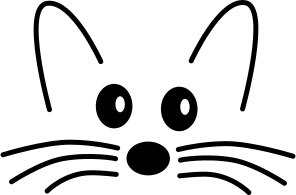
\includegraphics[width=1.4em]{squeak-logo}}}
\iftoshelse{
	\usepackage{marginnote}
		\renewcommand*{\marginfont}{\footnotesize}
	\newcommand{\vartriangleout}{\ifthenelse{\isodd{\thepage}}{\vartriangleright}{\vartriangleleft}}
	\newcommand{\dothisicon}{\fcolorbox{blue!65}{white}{\highlight{$\vartriangleout$}}}
	\newcommand{\dothis}[1]{%
		\noindent\par\noindent
		{\reversemarginpar
			\marginnote{\fcolorbox{blue!65}{white}{\highlight{$\vartriangleout$}}}}
		%\MarginLabel{do this}
		\noindent\emph{#1}
		\nopagebreak}
}{
	\newcommand{\dothisicon}{\raisebox{-.5ex}{
\includegraphics[height=1.2em]{pharo}}}
	\newcommand{\dothis}[1]{%
		\medskip
		\noindent\dothisicon
		\ifx#1\empty\else\quad\emph{#1}\fi
		\par\smallskip\nopagebreak}
}
%===> NEW VERSION <===
% NB: To use this in an individual chapter, you must set:
%\graphicspath{{figures/} {../figures/}}
% at the head of the chapter.  Don't forget the final /
%=============================================================
%:Reader hints (hint)
%
% Indicates a non-obvious consequence 
\newcommand{\hint}[1]{\vspace{1ex}\noindent\fbox{\textsc{Hint}} \emph{#1}}
%=================================================================
% graphics for Morphic handles
\newcommand{\grabHandle}{\raisebox{-0.2ex}{
\includegraphics[width=1em]{blackHandle}}}
\newcommand{\moveHandle}{\raisebox{-0.2ex}{
\includegraphics[width=1em]{moveHandle}}}
\newcommand{\debugHandle}{\raisebox{-0.2ex}{
\includegraphics[width=1em]{debugHandle}}}
%=============================================================
%:Highlighting Important stuff (doublebox)
%
% From Seaside book ...
\newsavebox{\SavedText}
\newlength{\InnerBoxRule}\setlength{\InnerBoxRule}{.75\fboxrule}
\newlength{\OuterBoxRule}\setlength{\OuterBoxRule}{1.5\fboxrule}
\newlength{\BoxSeparation}\setlength{\BoxSeparation}{1.5\fboxrule}
\addtolength{\BoxSeparation}{.5pt}
\newlength{\SaveBoxSep}\setlength{\SaveBoxSep}{2\fboxsep}
%
\newenvironment{doublebox}{\begin{lrbox}{\SavedText}
    \begin{minipage}{.75\textwidth}}
    {\end{minipage}\end{lrbox}\begin{center}
    \setlength{\fboxsep}{\BoxSeparation}\setlength{\fboxrule}{\OuterBoxRule}
    \fbox{\setlength{\fboxsep}{\SaveBoxSep}\setlength{\fboxrule}{\InnerBoxRule}%
      \fbox{\usebox{\SavedText}}}
  \end{center}}
% Use this:
\newcommand{\important}[1]{\begin{doublebox}#1\end{doublebox}}
%=============================================================
%:Section depth
\setcounter{secnumdepth}{2}
%% for this to happen start the file with
%\ifx\wholebook\relax\else
%% $Author$
% $Date$
% $Revision$

% HISTORY:
% 2006-10-31 - Oscar code macros
% ...

%=============================================================
% NB: documentclass must be set in main document.
% Allows book to be generated in multiple formats.
%=============================================================
%:Packages
\usepackage[T1]{fontenc}  %%%%%% really important to get the code directly in the text!
\usepackage{lmodern}
%\usepackage[scaled=0.85]{bookmanx} % needs another scale factor if used with \renewcommand{\sfdefault}{cmbr}
\usepackage{palatino}
\usepackage[scaled=0.85]{helvet}
\usepackage[protrusion,expansion=false]{microtype}
\usepackage{graphicx}
\usepackage{theorem}
\usepackage[english]{babel}
% ON: pdfsync breaks the use of p{width} for tabular columns!
\ifdefined\usepdfsync\usepackage{pdfsync}\fi % Requires texlive 2007
%=============================================================
%:More packages
%Stef should check which ones are used!
%\usepackage{picinpar}
%\usepackage{layout}
%\usepackage{color}
%\usepackage{enum}
%\usepackage{a4wide}
% \usepackage{fancyhdr}
\usepackage{ifthen}
\usepackage{float}
\usepackage{longtable}
\usepackage{makeidx}
\usepackage[nottoc]{tocbibind}
\usepackage{multicol}
\usepackage{booktabs}	% book-style tables
\usepackage{topcapt}	% enables \topcaption
\usepackage{multirow}
\usepackage{tabularx}
%\usepackage[bottom]{footmisc}
\usepackage{xspace}
\usepackage{alltt}
\usepackage{amssymb,textcomp}
\usepackage[usenames,dvipsnames]{color}
%\usepackage{colortbl}
\usepackage[hang]{subfigure}\makeatletter\def\p@subfigure{\thefigure\,}\makeatother
\usepackage{rotating}
\usepackage{enumitem}	% apb: allows more control over tags in enumerations
\usepackage{verbatim}     % for comment environment
\usepackage{varioref}	% for page references that work
\labelformat{footnote}{\thechapter--#1} % to distinguish citations from jurabib
\usepackage{needspace}
\usepackage{isodateo} % enable \isodate
\usepackage[newparttoc]{titlesec}
\usepackage{titletoc}
\usepackage{wrapfig}
\usepackage[
	super,
	citefull=first,
	authorformat={allreversed,and},
	titleformat={commasep,italic}
]{jurabib} % citations as footnotes
\usepackage[
	colorlinks=true,
	linkcolor=black,
	urlcolor=black,
	citecolor=black
]{hyperref}   % should come last
%=============================================================
%:PDF version
\pdfminorversion=3 % Set PDF to 1.3 for Lulu
%=============================================================
%:URL style
\makeatletter
\def\url@leostyle{%
  \@ifundefined{selectfont}{\def\UrlFont{\sf}}{\def\UrlFont{\sffamily}}}
\makeatother
% Now actually use the newly defined style.
\urlstyle{leo}
%=============================================================
%:Booleans
\newboolean{lulu}
\setboolean{lulu}{false}
\newcommand{\ifluluelse}[2]{\ifthenelse{\boolean{lulu}}{#1}{#2}}
%=============================================================
%:Names
\newcommand{\SUnit}{SUnit\xspace}
\newcommand{\sunit}{SUnit\xspace}
\newcommand{\xUnit}{$x$Unit\xspace}
\newcommand{\JUnit}{JUnit\xspace}
\newcommand{\st}{Smalltalk\xspace}
\newcommand{\pharo}{Pharo\xspace} % Use this, not \Pharo
%\newcommand{\sqmap}{SqueakMap\xspace}
\newcommand{\squeak}{Squeak\xspace} % use this, not \Squeak or \sq
\newcommand{\sqsrc}{SqueakSource\xspace}
\newcommand{\sbe}{\url{http://SqueakByExample.org}\xspace}
\newcommand{\pharoweb}{\url{http://pharo-project.org}\xspace}
\newcommand{\pbe}{\url{http://PharoByExample.org}\xspace}
\newcommand{\sba}{\url{http://SquareBracketAssociates.org}\xspace}
\newcommand{\bam}{\lct{Bounc\-ing\-Atoms\-Morph}\xspace}
%=============================================================
%:Markup macros for proof-reading
\usepackage[normalem]{ulem} % for \sout
\usepackage{xcolor}
\newcommand{\ra}{$\rightarrow$}
\newcommand{\ugh}[1]{\textcolor{red}{\uwave{#1}}} % please rephrase
\newcommand{\ins}[1]{\textcolor{blue}{\uline{#1}}} % please insert
\newcommand{\del}[1]{\textcolor{red}{\sout{#1}}} % please delete
\newcommand{\chg}[2]{\textcolor{red}{\sout{#1}}{\ra}\textcolor{blue}{\uline{#2}}} % please change
%=============================================================
%:Editorial comment macros
%\newcommand{\nnbb}[2]{
%    % \fbox{\bfseries\sffamily\scriptsize#1}
%    \fcolorbox{gray}{yellow}{\bfseries\sffamily\scriptsize#1}
%    {\sf\small$\blacktriangleright$\textit{#2}$\blacktriangleleft$}
%   }
\newcommand{\yellowbox}[1]{\fcolorbox{gray}{yellow}{\bfseries\sffamily\scriptsize#1}}
\newcommand{\triangles}[1]{{\sf\small$\blacktriangleright$\textit{#1}$\blacktriangleleft$}}
\newcommand{\nnbb}[2]{\yellowbox{#1} \triangles{#2}}
\newcommand{\fix}{\yellowbox{FIX!}}
\newcommand{\here}{\yellowbox{CONTINUE HERE!}}
% editor macros
\newcommand{\apl}[1]{\nnbb{Alain}{#1}} % Alain
\newcommand{\ab}[1]{\nnbb{Andrew}{#1}} % Black
\newcommand{\sd}[1]{\nnbb{St\'{e}f}{#1}} % Ducasse
\newcommand{\dc}[1]{\nnbb{DamienC}{#1}} % Ducasse
\newcommand{\md}[1]{\nnbb{Marcus}{#1}} % Denker
\newcommand{\on}[1]{\nnbb{Oscar}{#1}} % Nierstrasz
\newcommand{\damien}[1]{\nnbb{Damien}{#1}} % Pollet
\newcommand{\lr}[1]{\nnbb{Lukas}{#1}} % Renggli
\newcommand{\orla}[1]{\nnbb{Orla}{#1}} % Greevy
\newcommand{\alex}[1]{\nnbb{Alex}{#1}} % Bergel
\newcommand{\alx}[1]{\nnbb{Alex}{#1}} % Bergel
\newcommand{\dr}[1]{\nnbb{David}{#1}} % Roethlisberger
\newcommand{\ja}[1]{\nnbb{Jannik}{#1}} % Laval
\newcommand{\jr}[1]{\nnbb{Jorge}{#1}} % Ressia
\newcommand{\jb}[1]{\nnbb{JB}{#1}} % JB
\newcommand{\fp}[1]{\nnbb{Fabrizio}{#1}} % Perin
\newcommand{\michael}[1]{\nnbb{Michael}{#1}} % Davies
\newcommand{\ew}[1]{\nnbb{Erwann}{#1}} % Wernli
\newcommand{\mb}[1]{\nnbb{Martial}{#1}} % Boniou
\newcommand{\hw}[1]{\nnbb{Hernan}{#1}} % Wilkinson
\newcommand{\ben}[1]{\nnbb{Benjamin}{#1}} % Benjamin Van Ryseghem
%=============================================================
%:Abbreviation macros
\newcommand{\ie}{\emph{i.e.},\xspace}
\newcommand{\eg}{\emph{e.g.},\xspace}
\newcommand{\etc}{etc.\xspace}
%=============================================================
%:Cross reference macros
\newcommand{\charef}[1]{Chapter~\ref{cha:#1}\xspace}
\newcommand{\secref}[1]{Section~\ref{sec:#1}\xspace}
\newcommand{\figref}[1]{Figure~\ref{fig:#1}\xspace}
\newcommand{\Figref}[1]{Figure~\ref{fig:#1}\xspace}
\newcommand{\appref}[1]{Appendix~\ref{app:#1}\xspace}
\newcommand{\tabref}[1]{Table~\ref{tab:#1}\xspace}
\newcommand{\faqref}[1]{FAQ~\ref{faq:#1}, p.~\pageref{faq:#1}\xspace}
% APB: I removed trailing \xspace commands from these macros because
% \xspace mostly doesn't work.  If you want a space after your
% references, type one!
% ON: xspace has always worked just fine for me!  Please leave them in.
%
\newcommand{\ruleref}[1]{\ref{rule:#1}\xspace}
%
\newcommand{\egref}[1]{example~\ref{eg:#1}\xspace}
\newcommand{\Egref}[1]{Example~\ref{eg:#1}\xspace}
%
\newcommand{\scrref}[1]{script~\ref{scr:#1}\xspace}
\newcommand{\Scrref}[1]{Script~\ref{scr:#1}\xspace}
\newcommand{\tscrref}[1]{the script~\ref{scr:#1}\xspace}
\newcommand{\Tscrref}[1]{The script~\ref{scr:#1}\xspace}
%
\newcommand{\mthref}[1]{method~\ref{mth:#1}\xspace}
\newcommand{\mthsref}[1]{methods~\ref{mth:#1}\xspace}
\newcommand{\Mthref}[1]{Method~\ref{mth:#1}\xspace}
\newcommand{\tmthref}[1]{the method~\ref{mth:#1}\xspace}
\newcommand{\Tmthref}[1]{The method~\ref{mth:#1}\xspace}
%
\newcommand{\clsref}[1]{class~\ref{cls:#1}\xspace}
\newcommand{\tclsref}[1]{the class~\ref{cls:#1}\xspace}
\newcommand{\Tclsref}[1]{The class~\ref{cls:#1}\xspace}

\newcommand{\chalabel}[1]{\label{cha:#1}}
\newcommand{\seclabel}[1]{\label{sec:#1}}
\newcommand{\figlabel}[1]{\label{fig:#1}}
\newcommand{\tablabel}[1]{\label{tab:#1}}
\newcommand{\rulelabel}[1]{\label{rule:#1}}
\newcommand{\eglabel}[1]{\label{eg:#1}}
\newcommand{\scrlabel}[1]{\label{scr:#1}}
\newcommand{\mthlabel}[1]{\label{mth:#1}}
\newcommand{\clslabel}[1]{\label{cls:#1}}
\newcommand{\faqlabel}[1]{\label{faq:#1}}
%=============================================================
%:Menu item macro
% for menu items, so we can change our minds on how to print them! (apb)
\definecolor{lightgray}{gray}{0.89}
\newcommand{\menu}[1]{{%
	\setlength{\fboxsep}{0pt}%
	\colorbox{lightgray}{{{\upshape\sffamily\strut \,#1\,}}}}}
\newcommand{\link}[1]{{%
	\fontfamily{lmr}\selectfont
 	\upshape{\sffamily \underline{#1}}}}
% For submenu items:
\newcommand{\go}{\,$\triangleright$\,}
% \newcommand{\go}{\,$\blacktriangleright$\,}
% For keyboard shortcuts:
%\newcommand{\short}[1]{\mbox{$\langle${\sc CMD}$\rangle$-#1}\xspace}
\newcommand{\short}[1]{\mbox{{\sc cmd}\hspace{0.08em}--\hspace{0.09em}#1}\xspace}
% For buttons:
\newcommand{\button}[1]{{%
	\setlength{\fboxsep}{0pt}%
	\fbox{{\upshape\sffamily\strut \,#1\,}}}}
% NB: The button macro does not work within captions -- incompatible with xcolor package :-(
\newcommand{\toolsflap}{\textit{Tools} flap\xspace}
%=============================================================
%:Mouse clicks
\newcommand{\click}{click\xspace} % RED
\newcommand{\actclick}{action-click\xspace} % YELLOW
\newcommand{\metaclick}{meta-click\xspace} % BLUE
\newcommand{\Click}{Click\xspace} % RED
\newcommand{\Actclick}{Action-click\xspace} % YELLOW
\newcommand{\Metaclick}{Meta-click\xspace} % BLUE
%=============================================================
%:ToSh macros
\newboolean{tosh}
\setboolean{tosh}{false}
\newcommand{\iftoshelse}[2]{\ifthenelse{\boolean{tosh}}{#1}{#2}}
%=============================================================
%:ToSh colors
%\newcommand{\highlightcolor}{\color{blue!65}}
%\newcommand{\boxcolor}{\color{gray!25}}
\newcommand{\highlight}[1]{\textcolor{blue!65}{#1}}
%\newcommand{\codecolor}{\color{blue!65}}
%%\setlength{\fboxrule}{2pt}
%\newcommand{\asPict}[1]{%
%	{\Large\highlight{#1}}}
%=============================================================
%:Reader cues (do this)
%
% Indicate something the reader should try out.
% \newcommand{\dothisicon}{\raisebox{-.5ex}{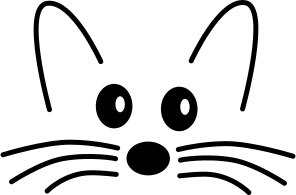
\includegraphics[width=1.4em]{squeak-logo}}}
\iftoshelse{
	\usepackage{marginnote}
		\renewcommand*{\marginfont}{\footnotesize}
	\newcommand{\vartriangleout}{\ifthenelse{\isodd{\thepage}}{\vartriangleright}{\vartriangleleft}}
	\newcommand{\dothisicon}{\fcolorbox{blue!65}{white}{\highlight{$\vartriangleout$}}}
	\newcommand{\dothis}[1]{%
		\noindent\par\noindent
		{\reversemarginpar
			\marginnote{\fcolorbox{blue!65}{white}{\highlight{$\vartriangleout$}}}}
		%\MarginLabel{do this}
		\noindent\emph{#1}
		\nopagebreak}
}{
	\newcommand{\dothisicon}{\raisebox{-.5ex}{
\includegraphics[height=1.2em]{pharo}}}
	\newcommand{\dothis}[1]{%
		\medskip
		\noindent\dothisicon
		\ifx#1\empty\else\quad\emph{#1}\fi
		\par\smallskip\nopagebreak}
}
%===> NEW VERSION <===
% NB: To use this in an individual chapter, you must set:
%\graphicspath{{figures/} {../figures/}}
% at the head of the chapter.  Don't forget the final /
%=============================================================
%:Reader hints (hint)
%
% Indicates a non-obvious consequence 
\newcommand{\hint}[1]{\vspace{1ex}\noindent\fbox{\textsc{Hint}} \emph{#1}}
%=================================================================
% graphics for Morphic handles
\newcommand{\grabHandle}{\raisebox{-0.2ex}{
\includegraphics[width=1em]{blackHandle}}}
\newcommand{\moveHandle}{\raisebox{-0.2ex}{
\includegraphics[width=1em]{moveHandle}}}
\newcommand{\debugHandle}{\raisebox{-0.2ex}{
\includegraphics[width=1em]{debugHandle}}}
%=============================================================
%:Highlighting Important stuff (doublebox)
%
% From Seaside book ...
\newsavebox{\SavedText}
\newlength{\InnerBoxRule}\setlength{\InnerBoxRule}{.75\fboxrule}
\newlength{\OuterBoxRule}\setlength{\OuterBoxRule}{1.5\fboxrule}
\newlength{\BoxSeparation}\setlength{\BoxSeparation}{1.5\fboxrule}
\addtolength{\BoxSeparation}{.5pt}
\newlength{\SaveBoxSep}\setlength{\SaveBoxSep}{2\fboxsep}
%
\newenvironment{doublebox}{\begin{lrbox}{\SavedText}
    \begin{minipage}{.75\textwidth}}
    {\end{minipage}\end{lrbox}\begin{center}
    \setlength{\fboxsep}{\BoxSeparation}\setlength{\fboxrule}{\OuterBoxRule}
    \fbox{\setlength{\fboxsep}{\SaveBoxSep}\setlength{\fboxrule}{\InnerBoxRule}%
      \fbox{\usebox{\SavedText}}}
  \end{center}}
% Use this:
\newcommand{\important}[1]{\begin{doublebox}#1\end{doublebox}}
%=============================================================
%:Section depth
\setcounter{secnumdepth}{2}
%% for this to happen start the file with
%\ifx\wholebook\relax\else
%\input{../common.tex}
%\begin{document}
%\fi
% and terminate by
% \ifx\wholebook\relax\else\end{document}\fi

\DeclareGraphicsExtensions{.pdf, .jpg, .png}
%=============================================================
%:PDF setup
\hypersetup{
%   a4paper,
%   pdfstartview=FitV,
%   colorlinks,
%   linkcolor=darkblue,
%   citecolor=darkblue,
   pdftitle={Pharo by Example},
   pdfauthor={Andrew P. Black, St\'ephane Ducasse,	Oscar Nierstrasz,
Damien Pollet},
   pdfkeywords={Smalltalk, Squeak, Object-Oriented Programming, OOP},
   pdfsubject={Computer Science}
}
%=============================================================
%:Page layout and appearance
%
% \renewcommand{\headrulewidth}{0pt}
\renewcommand{\chaptermark}[1]{\markboth{#1}{}}
\renewcommand{\sectionmark}[1]{\markright{\thesection\ #1}}
\renewpagestyle{plain}[\small\itshape]{%
	\setheadrule{0pt}%
	\sethead[][][]{}{}{}%
	\setfoot[][][]{}{}{}}
\renewpagestyle{headings}[\small\itshape]{%
	\setheadrule{0pt}%
	\setmarks{chapter}{section}%
	\sethead[\thepage][][\chaptertitle]{\sectiontitle}{}{\thepage}%
	\setfoot[][][]{}{}{}}
%=============================================================
%:Title section setup and TOC numbering depth
\setcounter{secnumdepth}{1}
\setcounter{tocdepth}{1}
\titleformat{\part}[display]{\centering}{\huge\partname\ \thepart}{1em}{\Huge\textbf}[]
\titleformat{\chapter}[display]{}{\huge\chaptertitlename\ \thechapter}{1em}{\Huge\raggedright\textbf}[]
\titlecontents{part}[3pc]{%
		\pagebreak[2]\addvspace{1em plus.4em minus.2em}%
		\leavevmode\large\bfseries}
	{\contentslabel{3pc}}{\hspace*{-3pc}}
	{}[\nopagebreak]
\titlecontents{chapter}[3pc]{%
		\pagebreak[0]\addvspace{1em plus.2em minus.2em}%
		\leavevmode\bfseries}
	{\contentslabel{3pc}}{}
	{\hfill\contentspage}[\nopagebreak]
\dottedcontents{section}[3pc]{}{3pc}{1pc}
\dottedcontents{subsection}[3pc]{}{0pc}{1pc}
% \dottedcontents{subsection}[4.5em]{}{0pt}{1pc}
% Make \cleardoublepage insert really blank pages http://www.tex.ac.uk/cgi-bin/texfaq2html?label=reallyblank
\let\origdoublepage\cleardoublepage
\newcommand{\clearemptydoublepage}{%
  \clearpage
  {\pagestyle{empty}\origdoublepage}}
\let\cleardoublepage\clearemptydoublepage % see http://www.tex.ac.uk/cgi-bin/texfaq2html?label=patch
%=============================================================
%:FAQ macros (for FAQ chapter)
\newtheorem{faq}{FAQ}
\newcommand{\answer}{\paragraph{Answer}\ }
%=============================================================
%:Listings package configuration
% \newcommand{\caret}{\makebox{\raisebox{0.4ex}{\footnotesize{$\wedge$}}}}
\newcommand{\caret}{\^\,}
\newcommand{\escape}{{\sf \textbackslash}}
\definecolor{source}{gray}{0.95}
\usepackage{listings}
\lstdefinelanguage{Smalltalk}{
%  morekeywords={self,super,true,false,nil,thisContext}, % This is overkill
  morestring=[d]',
  morecomment=[s]{"}{"},
  alsoletter={\#:},
  escapechar={!},
  literate=
    {BANG}{!}1
    {CARET}{\^}1
    {UNDERSCORE}{\_}1
    {\\st}{Smalltalk}9 % convenience -- in case \st occurs in code
    % {'}{{\textquotesingle}}1 % replaced by upquote=true in \lstset
    {_}{{$\leftarrow$}}1
    {>>>}{{\sep}}1
    {^}{{$\uparrow$}}1
    {~}{{$\sim$}}1
    {-}{{\texttt{-}}}1 %{\textminus}}1 %{-}{\hspace{-0.13em}}{-}}1  % the goal is to make - the same width as +
    % {+}{\sf+}1 %{\raisebox{0.08ex}{+}}}1      % and to raise + off the baseline to match -
    {-->}{{\quad$\longrightarrow$\quad}}3
	, % Don't forget the comma at the end!
  tabsize=4
}[keywords,comments,strings]

\lstset{language=Smalltalk,
	basicstyle=\sffamily,
	keywordstyle=\color{black}\bfseries,
	% stringstyle=\ttfamily, % Ugly! do we really want this? -- on
	mathescape=true,
	showstringspaces=false,
	keepspaces=true,
	breaklines=true,
	breakautoindent=true,
	backgroundcolor=\color{source},
	lineskip={-1pt}, % Ugly hack
	upquote=true, % straight quote; requires textcomp package
	columns=fullflexible} % no fixed width fonts
% In-line code (literal)
% Normally use this for all in-line code:
\newcommand{\ct}{\lstinline[mathescape=false,backgroundcolor=\color{white},basicstyle={\sffamily\upshape}]}
% apb 2007.8.28 added the \upshape declaration to avoid getting italicized code in \dothis{ } sections.
% In-line code (latex enabled)
% Use this only in special situations where \ct does not work
% (within section headings ...):
\newcommand{\lct}[1]{{\textsf{\textup{#1}}}}
% Use these for system categories and protocols:
\newcommand{\scat}[1]{\emph{\textsf{#1}}\xspace}
\newcommand{\pkg}[1]{\emph{\textsf{#1}}\xspace}
\newcommand{\prot}[1]{\emph{\textsf{#1}}\xspace}
% Code environments
% NB: the arg is for tests
% Only code and example environments may be tests
\lstnewenvironment{code}[1]{%
	\lstset{%
		% frame=lines,
		frame=single,
		framerule=0pt,
		mathescape=false
	}
}{}
\def\ignoredollar#1{}
%=============================================================
%:Code environments (method, script ...)
% NB: the third arg is for tests
% Only code and example environments may be tests
\lstnewenvironment{example}[3][defaultlabel]{%
	\renewcommand{\lstlistingname}{Example}%
	\lstset{
		% frame=lines,
		frame=single,
		framerule=0pt,
		mathescape=false,
		caption={\emph{#2}},
		label={eg:#1}
	}
}{}
\lstnewenvironment{script}[2][defaultlabel]{%
\renewcommand{\lstlistingname}{Script}%
	\lstset{
		% frame=lines,
		frame=single,
		framerule=0pt,
		mathescape=false,
		name={Script},
		caption={\emph{#2}},
		label={scr:#1}
	}
}{}
\lstnewenvironment{method}[2][defaultlabel]{%
	\renewcommand{\lstlistingname}{Method}%
	\lstset{
		% frame=lines,
		frame=single,
		framerule=0pt,
		mathescape=false,
		name={Method},
		caption={\emph{#2}},
		label={mth:#1}
	}
}{}
\lstnewenvironment{methods}[2][defaultlabel]{% just for multiple methods at once
	\renewcommand{\lstlistingname}{Methods}%
	\lstset{
		% frame=lines,
		frame=single,
		framerule=0pt,
		mathescape=false,
		name={Method},
		caption={\emph{#2}},
		label={mth:#1}
	}
}{}
\lstnewenvironment{numMethod}[2][defaultlabel]{%
	\renewcommand{\lstlistingname}{Method}%
	\lstset{
		numbers=left,
		numberstyle={\tiny\sffamily},
		% frame=lines,
		frame=single,
		framerule=0pt,
		mathescape=false,
		name={Method},
		caption={\emph{#2}},
		label={mth:#1}
	}
}{}
\lstnewenvironment{classdef}[2][defaultlabel]{%
	\renewcommand{\lstlistingname}{Class}%
	\lstset{
		% frame=lines,
		frame=single,
		framerule=0pt,
		mathescape=false,
		name={Class},
		caption={\emph{#2}},
		label={cls:#1}
	}
}{}
%=============================================================
%:Reserving space
% Usually need one more line than the actual lines of code
\newcommand{\needlines}[1]{\Needspace{#1\baselineskip}}
%=============================================================
%:Indexing macros
% Macros ending with "ind" generate text as well as an index entry
% Macros ending with "index" *only* generate an index entry
\newcommand{\ind}[1]{\index{#1}#1\xspace} % plain text
\newcommand{\subind}[2]{\index{#1!#2}#2\xspace} % show #2, subindex under #1
\newcommand{\emphind}[1]{\index{#1}\emph{#1}\xspace} % emph #1
\newcommand{\emphsubind}[2]{\index{#1!#2}\emph{#2}\xspace} % show emph #2, subindex inder #1
\newcommand{\scatind}[1]{\index{#1@\textsf{#1} (category)}\scat{#1}} % category
\newcommand{\pkgind}[1]{\index{#1@\textsf{#1} (package)}\pkg{#1}} % package
\newcommand{\protind}[1]{\index{#1@\textsf{#1} (protocol)}\prot{#1}} % protocol
\newcommand{\clsind}[1]{\index{#1@\textsf{#1} (class)}\ct{#1}\xspace}
% \newcommand{\clsind}[1]{\index{#1!\#@(class)}\ct{#1}\xspace} % class
\newcommand{\clsindplural}[1]{\index{#1!\#@(class)}\ct{#1}s\xspace} % class
\newcommand{\cvind}[1]{\index{#1@\textsf{#1} (class variable)}\ct{#1}\xspace} % class var
\newcommand{\glbind}[1]{\index{#1@\textsf{#1} (global)}\ct{#1}\xspace} % global
\newcommand{\patind}[1]{\index{#1@#1 (pattern)}\ct{#1}\xspace} % pattern
\newcommand{\pvind}[1]{\index{#1@\textsf{#1} (pseudo variable)}\ct{#1}\xspace} % pseudo var
\newcommand{\clsmthind}[2]{\index{#1!#2@\ct{#2}}\ct{#1>>>#2}\xspace} % class + method name
\newcommand{\mthind}[2]{\index{#1!#2@\ct{#2}}\ct{#2}\xspace} % show method name only
\newcommand{\lmthind}[2]{\index{#1!#2@\ct{#2}}\lct{#2}\xspace} % show method name only
\newcommand{\cmind}[2]{\index{#1!#2@\ct{#2}}\ct{#1>>>#2}\xspace} % show class>>method
\newcommand{\lcmind}[2]{\index{#1!#2@\ct{#2}}\lct{#1>>>#2}\xspace} % show class>>method
\newcommand{\toolsflapind}{\index{Tools flap}\toolsflap} % index tools flap
% The following only generate an index entry:
% \newcommand{\clsindex}[1]{\index{#1@\textsf{#1} (class)}}
\newcommand{\clsindex}[1]{\index{#1!\#@(class)}} % class
\newcommand{\mthindex}[2]{\index{#1!#2@\ct{#2}}} % method
\newcommand{\cmindex}[2]{\index{#1!#2@\ct{#2}}} % class>>method
\newcommand{\cvindex}[1]{\index{#1@\textsf{#1} (class variable)}} % class var
\newcommand{\glbindex}[1]{\index{#1@\textsf{#1} (global)}}% global
\newcommand{\pvindex}[1]{\index{#1@\textsf{#1} (pseudo variable)}}% pseudo var
\newcommand{\seeindex}[2]{\index{#1|see{#2}}} % #1, see #2
\newcommand{\scatindex}[1]{\index{#1@\textsf{#1} (category)}} % category
\newcommand{\pkgindex}[1]{\index{#1@\textsf{#1} (package)}} % package
\newcommand{\protindex}[1]{\index{#1@\textsf{#1} (protocol)}} % protocol
% How can we have the main entry page numbers in bold yet not break the hyperlink?
\newcommand{\boldidx}[1]{{\bf #1}} % breaks hyperlink
%\newcommand{\indmain}[1]{\index{#1|boldidx}#1\xspace} % plain text, main entry
%\newcommand{\emphsubindmain}[2]{\index{#1!#2|boldidx}\emph{#2}\xspace} % subindex, main entry
%\newcommand{\subindmain}[2]{\index{#1!#2|boldidx}#2\xspace} % subindex, main entry
%\newcommand{\clsindmain}[1]{\index{#1@\textsf{#1} (class)|boldidx}\ct{#1}\xspace}
%\newcommand{\clsindmain}[1]{\index{#1!\#@(class)|boldidx}\ct{#1}\xspace} % class main
%\newcommand{\indexmain}[1]{\index{#1|boldidx}} % main index entry only
\newcommand{\indmain}[1]{\index{#1}#1\xspace} % The main index entry for this item
\newcommand{\emphsubindmain}[2]{\index{#1!#2}\emph{#2}\xspace} % subindex, main entry
\newcommand{\subindmain}[2]{\index{#1!#2}#2\xspace} % subindex, main entry
%\newcommand{\clsindmain}[1]{\index{#1@\textsf{#1} (class)}\ct{#1}\xspace}
\newcommand{\clsindmain}[1]{\index{#1!\#@(class)}\ct{#1}\xspace} % class main
\newcommand{\clsindexmain}[1]{\index{#1!\#@(class)}} % class main index only
\newcommand{\indexmain}[1]{\index{#1}} 
%=============================================================
%:Code macros
% some constants
\newcommand{\codesize}{\small}
\newcommand{\codefont}{\sffamily}
%\newcommand{\cat}[1]{\textit{In category #1}}%%To remove later
\newlength{\scriptindent}
\setlength{\scriptindent}{.3cm}
%% Method presentation constants
\newlength{\methodindent}
\newlength{\methodwordlength}
\newlength{\aftermethod}
\setlength{\methodindent}{0.2cm}
\settowidth{\methodwordlength}{\ M\'ethode\ }
%=============================================================
%:Smalltalk macros
%\newcommand{\sep}{{$\gg$}}
\newcommand{\sep}{\mbox{>>}}
\newcommand{\self}{\lct{self}\xspace}
\newcommand{\super}{\lct{super}\xspace}
\newcommand{\nil}{\lct{nil}\xspace}
%=============================================================
% be less conservative about float placement
% these commands are from http://www.tex.ac.uk/cgi-bin/texfaq2html?label=floats
\renewcommand{\topfraction}{.9}
\renewcommand{\bottomfraction}{.9}
\renewcommand{\textfraction}{.1}
\renewcommand{\floatpagefraction}{.85}
\renewcommand{\dbltopfraction}{.66}
\renewcommand{\dblfloatpagefraction}{.85}
\setcounter{topnumber}{9}
\setcounter{bottomnumber}{9}
\setcounter{totalnumber}{20}
\setcounter{dbltopnumber}{9}
%=============================================================
% Give information from each chapter's author
\newcommand{\contact}[2]{\textbf{#1} \textsf{(#2)}}

\newcommand{\chapterauthor}[1]{\emph{with the participation of:\\#1}\\}

\newcommand{\authornoury}{\contact{Noury Bouraqadi}{bouraqadi@gmail.com}}
\newcommand{\authordamienc}{\contact{Damien Cassou}{damien.cassou@gmail.com}}
\newcommand{\authoroscar}{\contact{Oscar Nierstrasz}{oscar.nierstrasz@acm.org}}
\newcommand{\authorsteph}{\contact{St\'ephane Ducasse}{stephane.ducasse@inria.fr}}
\newcommand{\authoralex}{\contact{Alexandre Bergel}{alexandre@bergel.eu}}
\newcommand{\authorolivier}{\contact{Olivier Auverlot}{olivier.auverlot@inria.fr}}
\newcommand{\authornicolas}{\contact{Nicolas Cellier}{nicolas.cellier.aka.nice@gmail.com}}
\newcommand{\authormarcus}{\contact{Marcus Denker}{marcus.denker@inria.fr}}
\newcommand{\authoralain}{\contact{Alain Plantec}{alain.plantec@univ-brest.fr}}
\newcommand{\authordale}{\contact{Dale Henrichs}{dale.henrichs@gemstone.com}}
\newcommand{\authormariano}{\contact{Mariano Martinez Peck}{marianopeck@gmail.com}}
\newcommand{\authorsven}{\contact{Sven Van Caekenberghe}{sven@beta9.be}}
\newcommand{\authorlukas}{\contact{Lukas Renggli}{renggli@gmail.com}}

%=============================================================
% apb doesn't like paragraphs to run in to each other without a break
\parskip 1ex
%=============================================================
%:Stuff to check, merge or deprecate
%\setlength{\marginparsep}{2mm}
%\renewcommand{\baselinestretch}{1.1}
%=============================================================

%\begin{document}
%\fi
% and terminate by
% \ifx\wholebook\relax\else\end{document}\fi

\DeclareGraphicsExtensions{.pdf, .jpg, .png}
%=============================================================
%:PDF setup
\hypersetup{
%   a4paper,
%   pdfstartview=FitV,
%   colorlinks,
%   linkcolor=darkblue,
%   citecolor=darkblue,
   pdftitle={Pharo by Example},
   pdfauthor={Andrew P. Black, St\'ephane Ducasse,	Oscar Nierstrasz,
Damien Pollet},
   pdfkeywords={Smalltalk, Squeak, Object-Oriented Programming, OOP},
   pdfsubject={Computer Science}
}
%=============================================================
%:Page layout and appearance
%
% \renewcommand{\headrulewidth}{0pt}
\renewcommand{\chaptermark}[1]{\markboth{#1}{}}
\renewcommand{\sectionmark}[1]{\markright{\thesection\ #1}}
\renewpagestyle{plain}[\small\itshape]{%
	\setheadrule{0pt}%
	\sethead[][][]{}{}{}%
	\setfoot[][][]{}{}{}}
\renewpagestyle{headings}[\small\itshape]{%
	\setheadrule{0pt}%
	\setmarks{chapter}{section}%
	\sethead[\thepage][][\chaptertitle]{\sectiontitle}{}{\thepage}%
	\setfoot[][][]{}{}{}}
%=============================================================
%:Title section setup and TOC numbering depth
\setcounter{secnumdepth}{1}
\setcounter{tocdepth}{1}
\titleformat{\part}[display]{\centering}{\huge\partname\ \thepart}{1em}{\Huge\textbf}[]
\titleformat{\chapter}[display]{}{\huge\chaptertitlename\ \thechapter}{1em}{\Huge\raggedright\textbf}[]
\titlecontents{part}[3pc]{%
		\pagebreak[2]\addvspace{1em plus.4em minus.2em}%
		\leavevmode\large\bfseries}
	{\contentslabel{3pc}}{\hspace*{-3pc}}
	{}[\nopagebreak]
\titlecontents{chapter}[3pc]{%
		\pagebreak[0]\addvspace{1em plus.2em minus.2em}%
		\leavevmode\bfseries}
	{\contentslabel{3pc}}{}
	{\hfill\contentspage}[\nopagebreak]
\dottedcontents{section}[3pc]{}{3pc}{1pc}
\dottedcontents{subsection}[3pc]{}{0pc}{1pc}
% \dottedcontents{subsection}[4.5em]{}{0pt}{1pc}
% Make \cleardoublepage insert really blank pages http://www.tex.ac.uk/cgi-bin/texfaq2html?label=reallyblank
\let\origdoublepage\cleardoublepage
\newcommand{\clearemptydoublepage}{%
  \clearpage
  {\pagestyle{empty}\origdoublepage}}
\let\cleardoublepage\clearemptydoublepage % see http://www.tex.ac.uk/cgi-bin/texfaq2html?label=patch
%=============================================================
%:FAQ macros (for FAQ chapter)
\newtheorem{faq}{FAQ}
\newcommand{\answer}{\paragraph{Answer}\ }
%=============================================================
%:Listings package configuration
% \newcommand{\caret}{\makebox{\raisebox{0.4ex}{\footnotesize{$\wedge$}}}}
\newcommand{\caret}{\^\,}
\newcommand{\escape}{{\sf \textbackslash}}
\definecolor{source}{gray}{0.95}
\usepackage{listings}
\lstdefinelanguage{Smalltalk}{
%  morekeywords={self,super,true,false,nil,thisContext}, % This is overkill
  morestring=[d]',
  morecomment=[s]{"}{"},
  alsoletter={\#:},
  escapechar={!},
  literate=
    {BANG}{!}1
    {CARET}{\^}1
    {UNDERSCORE}{\_}1
    {\\st}{Smalltalk}9 % convenience -- in case \st occurs in code
    % {'}{{\textquotesingle}}1 % replaced by upquote=true in \lstset
    {_}{{$\leftarrow$}}1
    {>>>}{{\sep}}1
    {^}{{$\uparrow$}}1
    {~}{{$\sim$}}1
    {-}{{\texttt{-}}}1 %{\textminus}}1 %{-}{\hspace{-0.13em}}{-}}1  % the goal is to make - the same width as +
    % {+}{\sf+}1 %{\raisebox{0.08ex}{+}}}1      % and to raise + off the baseline to match -
    {-->}{{\quad$\longrightarrow$\quad}}3
	, % Don't forget the comma at the end!
  tabsize=4
}[keywords,comments,strings]

\lstset{language=Smalltalk,
	basicstyle=\sffamily,
	keywordstyle=\color{black}\bfseries,
	% stringstyle=\ttfamily, % Ugly! do we really want this? -- on
	mathescape=true,
	showstringspaces=false,
	keepspaces=true,
	breaklines=true,
	breakautoindent=true,
	backgroundcolor=\color{source},
	lineskip={-1pt}, % Ugly hack
	upquote=true, % straight quote; requires textcomp package
	columns=fullflexible} % no fixed width fonts
% In-line code (literal)
% Normally use this for all in-line code:
\newcommand{\ct}{\lstinline[mathescape=false,backgroundcolor=\color{white},basicstyle={\sffamily\upshape}]}
% apb 2007.8.28 added the \upshape declaration to avoid getting italicized code in \dothis{ } sections.
% In-line code (latex enabled)
% Use this only in special situations where \ct does not work
% (within section headings ...):
\newcommand{\lct}[1]{{\textsf{\textup{#1}}}}
% Use these for system categories and protocols:
\newcommand{\scat}[1]{\emph{\textsf{#1}}\xspace}
\newcommand{\pkg}[1]{\emph{\textsf{#1}}\xspace}
\newcommand{\prot}[1]{\emph{\textsf{#1}}\xspace}
% Code environments
% NB: the arg is for tests
% Only code and example environments may be tests
\lstnewenvironment{code}[1]{%
	\lstset{%
		% frame=lines,
		frame=single,
		framerule=0pt,
		mathescape=false
	}
}{}
\def\ignoredollar#1{}
%=============================================================
%:Code environments (method, script ...)
% NB: the third arg is for tests
% Only code and example environments may be tests
\lstnewenvironment{example}[3][defaultlabel]{%
	\renewcommand{\lstlistingname}{Example}%
	\lstset{
		% frame=lines,
		frame=single,
		framerule=0pt,
		mathescape=false,
		caption={\emph{#2}},
		label={eg:#1}
	}
}{}
\lstnewenvironment{script}[2][defaultlabel]{%
\renewcommand{\lstlistingname}{Script}%
	\lstset{
		% frame=lines,
		frame=single,
		framerule=0pt,
		mathescape=false,
		name={Script},
		caption={\emph{#2}},
		label={scr:#1}
	}
}{}
\lstnewenvironment{method}[2][defaultlabel]{%
	\renewcommand{\lstlistingname}{Method}%
	\lstset{
		% frame=lines,
		frame=single,
		framerule=0pt,
		mathescape=false,
		name={Method},
		caption={\emph{#2}},
		label={mth:#1}
	}
}{}
\lstnewenvironment{methods}[2][defaultlabel]{% just for multiple methods at once
	\renewcommand{\lstlistingname}{Methods}%
	\lstset{
		% frame=lines,
		frame=single,
		framerule=0pt,
		mathescape=false,
		name={Method},
		caption={\emph{#2}},
		label={mth:#1}
	}
}{}
\lstnewenvironment{numMethod}[2][defaultlabel]{%
	\renewcommand{\lstlistingname}{Method}%
	\lstset{
		numbers=left,
		numberstyle={\tiny\sffamily},
		% frame=lines,
		frame=single,
		framerule=0pt,
		mathescape=false,
		name={Method},
		caption={\emph{#2}},
		label={mth:#1}
	}
}{}
\lstnewenvironment{classdef}[2][defaultlabel]{%
	\renewcommand{\lstlistingname}{Class}%
	\lstset{
		% frame=lines,
		frame=single,
		framerule=0pt,
		mathescape=false,
		name={Class},
		caption={\emph{#2}},
		label={cls:#1}
	}
}{}
%=============================================================
%:Reserving space
% Usually need one more line than the actual lines of code
\newcommand{\needlines}[1]{\Needspace{#1\baselineskip}}
%=============================================================
%:Indexing macros
% Macros ending with "ind" generate text as well as an index entry
% Macros ending with "index" *only* generate an index entry
\newcommand{\ind}[1]{\index{#1}#1\xspace} % plain text
\newcommand{\subind}[2]{\index{#1!#2}#2\xspace} % show #2, subindex under #1
\newcommand{\emphind}[1]{\index{#1}\emph{#1}\xspace} % emph #1
\newcommand{\emphsubind}[2]{\index{#1!#2}\emph{#2}\xspace} % show emph #2, subindex inder #1
\newcommand{\scatind}[1]{\index{#1@\textsf{#1} (category)}\scat{#1}} % category
\newcommand{\pkgind}[1]{\index{#1@\textsf{#1} (package)}\pkg{#1}} % package
\newcommand{\protind}[1]{\index{#1@\textsf{#1} (protocol)}\prot{#1}} % protocol
\newcommand{\clsind}[1]{\index{#1@\textsf{#1} (class)}\ct{#1}\xspace}
% \newcommand{\clsind}[1]{\index{#1!\#@(class)}\ct{#1}\xspace} % class
\newcommand{\clsindplural}[1]{\index{#1!\#@(class)}\ct{#1}s\xspace} % class
\newcommand{\cvind}[1]{\index{#1@\textsf{#1} (class variable)}\ct{#1}\xspace} % class var
\newcommand{\glbind}[1]{\index{#1@\textsf{#1} (global)}\ct{#1}\xspace} % global
\newcommand{\patind}[1]{\index{#1@#1 (pattern)}\ct{#1}\xspace} % pattern
\newcommand{\pvind}[1]{\index{#1@\textsf{#1} (pseudo variable)}\ct{#1}\xspace} % pseudo var
\newcommand{\clsmthind}[2]{\index{#1!#2@\ct{#2}}\ct{#1>>>#2}\xspace} % class + method name
\newcommand{\mthind}[2]{\index{#1!#2@\ct{#2}}\ct{#2}\xspace} % show method name only
\newcommand{\lmthind}[2]{\index{#1!#2@\ct{#2}}\lct{#2}\xspace} % show method name only
\newcommand{\cmind}[2]{\index{#1!#2@\ct{#2}}\ct{#1>>>#2}\xspace} % show class>>method
\newcommand{\lcmind}[2]{\index{#1!#2@\ct{#2}}\lct{#1>>>#2}\xspace} % show class>>method
\newcommand{\toolsflapind}{\index{Tools flap}\toolsflap} % index tools flap
% The following only generate an index entry:
% \newcommand{\clsindex}[1]{\index{#1@\textsf{#1} (class)}}
\newcommand{\clsindex}[1]{\index{#1!\#@(class)}} % class
\newcommand{\mthindex}[2]{\index{#1!#2@\ct{#2}}} % method
\newcommand{\cmindex}[2]{\index{#1!#2@\ct{#2}}} % class>>method
\newcommand{\cvindex}[1]{\index{#1@\textsf{#1} (class variable)}} % class var
\newcommand{\glbindex}[1]{\index{#1@\textsf{#1} (global)}}% global
\newcommand{\pvindex}[1]{\index{#1@\textsf{#1} (pseudo variable)}}% pseudo var
\newcommand{\seeindex}[2]{\index{#1|see{#2}}} % #1, see #2
\newcommand{\scatindex}[1]{\index{#1@\textsf{#1} (category)}} % category
\newcommand{\pkgindex}[1]{\index{#1@\textsf{#1} (package)}} % package
\newcommand{\protindex}[1]{\index{#1@\textsf{#1} (protocol)}} % protocol
% How can we have the main entry page numbers in bold yet not break the hyperlink?
\newcommand{\boldidx}[1]{{\bf #1}} % breaks hyperlink
%\newcommand{\indmain}[1]{\index{#1|boldidx}#1\xspace} % plain text, main entry
%\newcommand{\emphsubindmain}[2]{\index{#1!#2|boldidx}\emph{#2}\xspace} % subindex, main entry
%\newcommand{\subindmain}[2]{\index{#1!#2|boldidx}#2\xspace} % subindex, main entry
%\newcommand{\clsindmain}[1]{\index{#1@\textsf{#1} (class)|boldidx}\ct{#1}\xspace}
%\newcommand{\clsindmain}[1]{\index{#1!\#@(class)|boldidx}\ct{#1}\xspace} % class main
%\newcommand{\indexmain}[1]{\index{#1|boldidx}} % main index entry only
\newcommand{\indmain}[1]{\index{#1}#1\xspace} % The main index entry for this item
\newcommand{\emphsubindmain}[2]{\index{#1!#2}\emph{#2}\xspace} % subindex, main entry
\newcommand{\subindmain}[2]{\index{#1!#2}#2\xspace} % subindex, main entry
%\newcommand{\clsindmain}[1]{\index{#1@\textsf{#1} (class)}\ct{#1}\xspace}
\newcommand{\clsindmain}[1]{\index{#1!\#@(class)}\ct{#1}\xspace} % class main
\newcommand{\clsindexmain}[1]{\index{#1!\#@(class)}} % class main index only
\newcommand{\indexmain}[1]{\index{#1}} 
%=============================================================
%:Code macros
% some constants
\newcommand{\codesize}{\small}
\newcommand{\codefont}{\sffamily}
%\newcommand{\cat}[1]{\textit{In category #1}}%%To remove later
\newlength{\scriptindent}
\setlength{\scriptindent}{.3cm}
%% Method presentation constants
\newlength{\methodindent}
\newlength{\methodwordlength}
\newlength{\aftermethod}
\setlength{\methodindent}{0.2cm}
\settowidth{\methodwordlength}{\ M\'ethode\ }
%=============================================================
%:Smalltalk macros
%\newcommand{\sep}{{$\gg$}}
\newcommand{\sep}{\mbox{>>}}
\newcommand{\self}{\lct{self}\xspace}
\newcommand{\super}{\lct{super}\xspace}
\newcommand{\nil}{\lct{nil}\xspace}
%=============================================================
% be less conservative about float placement
% these commands are from http://www.tex.ac.uk/cgi-bin/texfaq2html?label=floats
\renewcommand{\topfraction}{.9}
\renewcommand{\bottomfraction}{.9}
\renewcommand{\textfraction}{.1}
\renewcommand{\floatpagefraction}{.85}
\renewcommand{\dbltopfraction}{.66}
\renewcommand{\dblfloatpagefraction}{.85}
\setcounter{topnumber}{9}
\setcounter{bottomnumber}{9}
\setcounter{totalnumber}{20}
\setcounter{dbltopnumber}{9}
%=============================================================
% Give information from each chapter's author
\newcommand{\contact}[2]{\textbf{#1} \textsf{(#2)}}

\newcommand{\chapterauthor}[1]{\emph{with the participation of:\\#1}\\}

\newcommand{\authornoury}{\contact{Noury Bouraqadi}{bouraqadi@gmail.com}}
\newcommand{\authordamienc}{\contact{Damien Cassou}{damien.cassou@gmail.com}}
\newcommand{\authoroscar}{\contact{Oscar Nierstrasz}{oscar.nierstrasz@acm.org}}
\newcommand{\authorsteph}{\contact{St\'ephane Ducasse}{stephane.ducasse@inria.fr}}
\newcommand{\authoralex}{\contact{Alexandre Bergel}{alexandre@bergel.eu}}
\newcommand{\authorolivier}{\contact{Olivier Auverlot}{olivier.auverlot@inria.fr}}
\newcommand{\authornicolas}{\contact{Nicolas Cellier}{nicolas.cellier.aka.nice@gmail.com}}
\newcommand{\authormarcus}{\contact{Marcus Denker}{marcus.denker@inria.fr}}
\newcommand{\authoralain}{\contact{Alain Plantec}{alain.plantec@univ-brest.fr}}
\newcommand{\authordale}{\contact{Dale Henrichs}{dale.henrichs@gemstone.com}}
\newcommand{\authormariano}{\contact{Mariano Martinez Peck}{marianopeck@gmail.com}}
\newcommand{\authorsven}{\contact{Sven Van Caekenberghe}{sven@beta9.be}}
\newcommand{\authorlukas}{\contact{Lukas Renggli}{renggli@gmail.com}}

%=============================================================
% apb doesn't like paragraphs to run in to each other without a break
\parskip 1ex
%=============================================================
%:Stuff to check, merge or deprecate
%\setlength{\marginparsep}{2mm}
%\renewcommand{\baselinestretch}{1.1}
%=============================================================

%\begin{document}
%\fi
% and terminate by
% \ifx\wholebook\relax\else\end{document}\fi

\DeclareGraphicsExtensions{.pdf, .jpg, .png}
%=============================================================
%:PDF setup
\hypersetup{
%   a4paper,
%   pdfstartview=FitV,
%   colorlinks,
%   linkcolor=darkblue,
%   citecolor=darkblue,
   pdftitle={Pharo by Example},
   pdfauthor={Andrew P. Black, St\'ephane Ducasse,	Oscar Nierstrasz,
Damien Pollet},
   pdfkeywords={Smalltalk, Squeak, Object-Oriented Programming, OOP},
   pdfsubject={Computer Science}
}
%=============================================================
%:Page layout and appearance
%
% \renewcommand{\headrulewidth}{0pt}
\renewcommand{\chaptermark}[1]{\markboth{#1}{}}
\renewcommand{\sectionmark}[1]{\markright{\thesection\ #1}}
\renewpagestyle{plain}[\small\itshape]{%
	\setheadrule{0pt}%
	\sethead[][][]{}{}{}%
	\setfoot[][][]{}{}{}}
\renewpagestyle{headings}[\small\itshape]{%
	\setheadrule{0pt}%
	\setmarks{chapter}{section}%
	\sethead[\thepage][][\chaptertitle]{\sectiontitle}{}{\thepage}%
	\setfoot[][][]{}{}{}}
%=============================================================
%:Title section setup and TOC numbering depth
\setcounter{secnumdepth}{1}
\setcounter{tocdepth}{1}
\titleformat{\part}[display]{\centering}{\huge\partname\ \thepart}{1em}{\Huge\textbf}[]
\titleformat{\chapter}[display]{}{\huge\chaptertitlename\ \thechapter}{1em}{\Huge\raggedright\textbf}[]
\titlecontents{part}[3pc]{%
		\pagebreak[2]\addvspace{1em plus.4em minus.2em}%
		\leavevmode\large\bfseries}
	{\contentslabel{3pc}}{\hspace*{-3pc}}
	{}[\nopagebreak]
\titlecontents{chapter}[3pc]{%
		\pagebreak[0]\addvspace{1em plus.2em minus.2em}%
		\leavevmode\bfseries}
	{\contentslabel{3pc}}{}
	{\hfill\contentspage}[\nopagebreak]
\dottedcontents{section}[3pc]{}{3pc}{1pc}
\dottedcontents{subsection}[3pc]{}{0pc}{1pc}
% \dottedcontents{subsection}[4.5em]{}{0pt}{1pc}
% Make \cleardoublepage insert really blank pages http://www.tex.ac.uk/cgi-bin/texfaq2html?label=reallyblank
\let\origdoublepage\cleardoublepage
\newcommand{\clearemptydoublepage}{%
  \clearpage
  {\pagestyle{empty}\origdoublepage}}
\let\cleardoublepage\clearemptydoublepage % see http://www.tex.ac.uk/cgi-bin/texfaq2html?label=patch
%=============================================================
%:FAQ macros (for FAQ chapter)
\newtheorem{faq}{FAQ}
\newcommand{\answer}{\paragraph{Answer}\ }
%=============================================================
%:Listings package configuration
% \newcommand{\caret}{\makebox{\raisebox{0.4ex}{\footnotesize{$\wedge$}}}}
\newcommand{\caret}{\^\,}
\newcommand{\escape}{{\sf \textbackslash}}
\definecolor{source}{gray}{0.95}
\usepackage{listings}
\lstdefinelanguage{Smalltalk}{
%  morekeywords={self,super,true,false,nil,thisContext}, % This is overkill
  morestring=[d]',
  morecomment=[s]{"}{"},
  alsoletter={\#:},
  escapechar={!},
  literate=
    {BANG}{!}1
    {CARET}{\^}1
    {UNDERSCORE}{\_}1
    {\\st}{Smalltalk}9 % convenience -- in case \st occurs in code
    % {'}{{\textquotesingle}}1 % replaced by upquote=true in \lstset
    {_}{{$\leftarrow$}}1
    {>>>}{{\sep}}1
    {^}{{$\uparrow$}}1
    {~}{{$\sim$}}1
    {-}{{\texttt{-}}}1 %{\textminus}}1 %{-}{\hspace{-0.13em}}{-}}1  % the goal is to make - the same width as +
    % {+}{\sf+}1 %{\raisebox{0.08ex}{+}}}1      % and to raise + off the baseline to match -
    {-->}{{\quad$\longrightarrow$\quad}}3
	, % Don't forget the comma at the end!
  tabsize=4
}[keywords,comments,strings]

\lstset{language=Smalltalk,
	basicstyle=\sffamily,
	keywordstyle=\color{black}\bfseries,
	% stringstyle=\ttfamily, % Ugly! do we really want this? -- on
	mathescape=true,
	showstringspaces=false,
	keepspaces=true,
	breaklines=true,
	breakautoindent=true,
	backgroundcolor=\color{source},
	lineskip={-1pt}, % Ugly hack
	upquote=true, % straight quote; requires textcomp package
	columns=fullflexible} % no fixed width fonts
% In-line code (literal)
% Normally use this for all in-line code:
\newcommand{\ct}{\lstinline[mathescape=false,backgroundcolor=\color{white},basicstyle={\sffamily\upshape}]}
% apb 2007.8.28 added the \upshape declaration to avoid getting italicized code in \dothis{ } sections.
% In-line code (latex enabled)
% Use this only in special situations where \ct does not work
% (within section headings ...):
\newcommand{\lct}[1]{{\textsf{\textup{#1}}}}
% Use these for system categories and protocols:
\newcommand{\scat}[1]{\emph{\textsf{#1}}\xspace}
\newcommand{\pkg}[1]{\emph{\textsf{#1}}\xspace}
\newcommand{\prot}[1]{\emph{\textsf{#1}}\xspace}
% Code environments
% NB: the arg is for tests
% Only code and example environments may be tests
\lstnewenvironment{code}[1]{%
	\lstset{%
		% frame=lines,
		frame=single,
		framerule=0pt,
		mathescape=false
	}
}{}
\def\ignoredollar#1{}
%=============================================================
%:Code environments (method, script ...)
% NB: the third arg is for tests
% Only code and example environments may be tests
\lstnewenvironment{example}[3][defaultlabel]{%
	\renewcommand{\lstlistingname}{Example}%
	\lstset{
		% frame=lines,
		frame=single,
		framerule=0pt,
		mathescape=false,
		caption={\emph{#2}},
		label={eg:#1}
	}
}{}
\lstnewenvironment{script}[2][defaultlabel]{%
\renewcommand{\lstlistingname}{Script}%
	\lstset{
		% frame=lines,
		frame=single,
		framerule=0pt,
		mathescape=false,
		name={Script},
		caption={\emph{#2}},
		label={scr:#1}
	}
}{}
\lstnewenvironment{method}[2][defaultlabel]{%
	\renewcommand{\lstlistingname}{Method}%
	\lstset{
		% frame=lines,
		frame=single,
		framerule=0pt,
		mathescape=false,
		name={Method},
		caption={\emph{#2}},
		label={mth:#1}
	}
}{}
\lstnewenvironment{methods}[2][defaultlabel]{% just for multiple methods at once
	\renewcommand{\lstlistingname}{Methods}%
	\lstset{
		% frame=lines,
		frame=single,
		framerule=0pt,
		mathescape=false,
		name={Method},
		caption={\emph{#2}},
		label={mth:#1}
	}
}{}
\lstnewenvironment{numMethod}[2][defaultlabel]{%
	\renewcommand{\lstlistingname}{Method}%
	\lstset{
		numbers=left,
		numberstyle={\tiny\sffamily},
		% frame=lines,
		frame=single,
		framerule=0pt,
		mathescape=false,
		name={Method},
		caption={\emph{#2}},
		label={mth:#1}
	}
}{}
\lstnewenvironment{classdef}[2][defaultlabel]{%
	\renewcommand{\lstlistingname}{Class}%
	\lstset{
		% frame=lines,
		frame=single,
		framerule=0pt,
		mathescape=false,
		name={Class},
		caption={\emph{#2}},
		label={cls:#1}
	}
}{}
%=============================================================
%:Reserving space
% Usually need one more line than the actual lines of code
\newcommand{\needlines}[1]{\Needspace{#1\baselineskip}}
%=============================================================
%:Indexing macros
% Macros ending with "ind" generate text as well as an index entry
% Macros ending with "index" *only* generate an index entry
\newcommand{\ind}[1]{\index{#1}#1\xspace} % plain text
\newcommand{\subind}[2]{\index{#1!#2}#2\xspace} % show #2, subindex under #1
\newcommand{\emphind}[1]{\index{#1}\emph{#1}\xspace} % emph #1
\newcommand{\emphsubind}[2]{\index{#1!#2}\emph{#2}\xspace} % show emph #2, subindex inder #1
\newcommand{\scatind}[1]{\index{#1@\textsf{#1} (category)}\scat{#1}} % category
\newcommand{\pkgind}[1]{\index{#1@\textsf{#1} (package)}\pkg{#1}} % package
\newcommand{\protind}[1]{\index{#1@\textsf{#1} (protocol)}\prot{#1}} % protocol
\newcommand{\clsind}[1]{\index{#1@\textsf{#1} (class)}\ct{#1}\xspace}
% \newcommand{\clsind}[1]{\index{#1!\#@(class)}\ct{#1}\xspace} % class
\newcommand{\clsindplural}[1]{\index{#1!\#@(class)}\ct{#1}s\xspace} % class
\newcommand{\cvind}[1]{\index{#1@\textsf{#1} (class variable)}\ct{#1}\xspace} % class var
\newcommand{\glbind}[1]{\index{#1@\textsf{#1} (global)}\ct{#1}\xspace} % global
\newcommand{\patind}[1]{\index{#1@#1 (pattern)}\ct{#1}\xspace} % pattern
\newcommand{\pvind}[1]{\index{#1@\textsf{#1} (pseudo variable)}\ct{#1}\xspace} % pseudo var
\newcommand{\clsmthind}[2]{\index{#1!#2@\ct{#2}}\ct{#1>>>#2}\xspace} % class + method name
\newcommand{\mthind}[2]{\index{#1!#2@\ct{#2}}\ct{#2}\xspace} % show method name only
\newcommand{\lmthind}[2]{\index{#1!#2@\ct{#2}}\lct{#2}\xspace} % show method name only
\newcommand{\cmind}[2]{\index{#1!#2@\ct{#2}}\ct{#1>>>#2}\xspace} % show class>>method
\newcommand{\lcmind}[2]{\index{#1!#2@\ct{#2}}\lct{#1>>>#2}\xspace} % show class>>method
\newcommand{\toolsflapind}{\index{Tools flap}\toolsflap} % index tools flap
% The following only generate an index entry:
% \newcommand{\clsindex}[1]{\index{#1@\textsf{#1} (class)}}
\newcommand{\clsindex}[1]{\index{#1!\#@(class)}} % class
\newcommand{\mthindex}[2]{\index{#1!#2@\ct{#2}}} % method
\newcommand{\cmindex}[2]{\index{#1!#2@\ct{#2}}} % class>>method
\newcommand{\cvindex}[1]{\index{#1@\textsf{#1} (class variable)}} % class var
\newcommand{\glbindex}[1]{\index{#1@\textsf{#1} (global)}}% global
\newcommand{\pvindex}[1]{\index{#1@\textsf{#1} (pseudo variable)}}% pseudo var
\newcommand{\seeindex}[2]{\index{#1|see{#2}}} % #1, see #2
\newcommand{\scatindex}[1]{\index{#1@\textsf{#1} (category)}} % category
\newcommand{\pkgindex}[1]{\index{#1@\textsf{#1} (package)}} % package
\newcommand{\protindex}[1]{\index{#1@\textsf{#1} (protocol)}} % protocol
% How can we have the main entry page numbers in bold yet not break the hyperlink?
\newcommand{\boldidx}[1]{{\bf #1}} % breaks hyperlink
%\newcommand{\indmain}[1]{\index{#1|boldidx}#1\xspace} % plain text, main entry
%\newcommand{\emphsubindmain}[2]{\index{#1!#2|boldidx}\emph{#2}\xspace} % subindex, main entry
%\newcommand{\subindmain}[2]{\index{#1!#2|boldidx}#2\xspace} % subindex, main entry
%\newcommand{\clsindmain}[1]{\index{#1@\textsf{#1} (class)|boldidx}\ct{#1}\xspace}
%\newcommand{\clsindmain}[1]{\index{#1!\#@(class)|boldidx}\ct{#1}\xspace} % class main
%\newcommand{\indexmain}[1]{\index{#1|boldidx}} % main index entry only
\newcommand{\indmain}[1]{\index{#1}#1\xspace} % The main index entry for this item
\newcommand{\emphsubindmain}[2]{\index{#1!#2}\emph{#2}\xspace} % subindex, main entry
\newcommand{\subindmain}[2]{\index{#1!#2}#2\xspace} % subindex, main entry
%\newcommand{\clsindmain}[1]{\index{#1@\textsf{#1} (class)}\ct{#1}\xspace}
\newcommand{\clsindmain}[1]{\index{#1!\#@(class)}\ct{#1}\xspace} % class main
\newcommand{\clsindexmain}[1]{\index{#1!\#@(class)}} % class main index only
\newcommand{\indexmain}[1]{\index{#1}} 
%=============================================================
%:Code macros
% some constants
\newcommand{\codesize}{\small}
\newcommand{\codefont}{\sffamily}
%\newcommand{\cat}[1]{\textit{In category #1}}%%To remove later
\newlength{\scriptindent}
\setlength{\scriptindent}{.3cm}
%% Method presentation constants
\newlength{\methodindent}
\newlength{\methodwordlength}
\newlength{\aftermethod}
\setlength{\methodindent}{0.2cm}
\settowidth{\methodwordlength}{\ M\'ethode\ }
%=============================================================
%:Smalltalk macros
%\newcommand{\sep}{{$\gg$}}
\newcommand{\sep}{\mbox{>>}}
\newcommand{\self}{\lct{self}\xspace}
\newcommand{\super}{\lct{super}\xspace}
\newcommand{\nil}{\lct{nil}\xspace}
%=============================================================
% be less conservative about float placement
% these commands are from http://www.tex.ac.uk/cgi-bin/texfaq2html?label=floats
\renewcommand{\topfraction}{.9}
\renewcommand{\bottomfraction}{.9}
\renewcommand{\textfraction}{.1}
\renewcommand{\floatpagefraction}{.85}
\renewcommand{\dbltopfraction}{.66}
\renewcommand{\dblfloatpagefraction}{.85}
\setcounter{topnumber}{9}
\setcounter{bottomnumber}{9}
\setcounter{totalnumber}{20}
\setcounter{dbltopnumber}{9}
%=============================================================
% Give information from each chapter's author
\newcommand{\contact}[2]{\textbf{#1} \textsf{(#2)}}

\newcommand{\chapterauthor}[1]{\emph{with the participation of:\\#1}\\}

\newcommand{\authornoury}{\contact{Noury Bouraqadi}{bouraqadi@gmail.com}}
\newcommand{\authordamienc}{\contact{Damien Cassou}{damien.cassou@gmail.com}}
\newcommand{\authoroscar}{\contact{Oscar Nierstrasz}{oscar.nierstrasz@acm.org}}
\newcommand{\authorsteph}{\contact{St\'ephane Ducasse}{stephane.ducasse@inria.fr}}
\newcommand{\authoralex}{\contact{Alexandre Bergel}{alexandre@bergel.eu}}
\newcommand{\authorolivier}{\contact{Olivier Auverlot}{olivier.auverlot@inria.fr}}
\newcommand{\authornicolas}{\contact{Nicolas Cellier}{nicolas.cellier.aka.nice@gmail.com}}
\newcommand{\authormarcus}{\contact{Marcus Denker}{marcus.denker@inria.fr}}
\newcommand{\authoralain}{\contact{Alain Plantec}{alain.plantec@univ-brest.fr}}
\newcommand{\authordale}{\contact{Dale Henrichs}{dale.henrichs@gemstone.com}}
\newcommand{\authormariano}{\contact{Mariano Martinez Peck}{marianopeck@gmail.com}}
\newcommand{\authorsven}{\contact{Sven Van Caekenberghe}{sven@beta9.be}}
\newcommand{\authorlukas}{\contact{Lukas Renggli}{renggli@gmail.com}}

%=============================================================
% apb doesn't like paragraphs to run in to each other without a break
\parskip 1ex
%=============================================================
%:Stuff to check, merge or deprecate
%\setlength{\marginparsep}{2mm}
%\renewcommand{\baselinestretch}{1.1}
%=============================================================

	\pagestyle{headings}
	\setboolean{lulu}{true}
% --------------------------------------------
% A4:
%	\documentclass[a4paper,11pt,twoside]{book}
%	% $Author$
% $Date$
% $Revision$

% HISTORY:
% 2006-10-31 - Oscar code macros
% ...

%=============================================================
% NB: documentclass must be set in main document.
% Allows book to be generated in multiple formats.
%=============================================================
%:Packages
\usepackage[T1]{fontenc}  %%%%%% really important to get the code directly in the text!
\usepackage{lmodern}
%\usepackage[scaled=0.85]{bookmanx} % needs another scale factor if used with \renewcommand{\sfdefault}{cmbr}
\usepackage{palatino}
\usepackage[scaled=0.85]{helvet}
\usepackage[protrusion,expansion=false]{microtype}
\usepackage{graphicx}
\usepackage{theorem}
\usepackage[english]{babel}
% ON: pdfsync breaks the use of p{width} for tabular columns!
\ifdefined\usepdfsync\usepackage{pdfsync}\fi % Requires texlive 2007
%=============================================================
%:More packages
%Stef should check which ones are used!
%\usepackage{picinpar}
%\usepackage{layout}
%\usepackage{color}
%\usepackage{enum}
%\usepackage{a4wide}
% \usepackage{fancyhdr}
\usepackage{ifthen}
\usepackage{float}
\usepackage{longtable}
\usepackage{makeidx}
\usepackage[nottoc]{tocbibind}
\usepackage{multicol}
\usepackage{booktabs}	% book-style tables
\usepackage{topcapt}	% enables \topcaption
\usepackage{multirow}
\usepackage{tabularx}
%\usepackage[bottom]{footmisc}
\usepackage{xspace}
\usepackage{alltt}
\usepackage{amssymb,textcomp}
\usepackage[usenames,dvipsnames]{color}
%\usepackage{colortbl}
\usepackage[hang]{subfigure}\makeatletter\def\p@subfigure{\thefigure\,}\makeatother
\usepackage{rotating}
\usepackage{enumitem}	% apb: allows more control over tags in enumerations
\usepackage{verbatim}     % for comment environment
\usepackage{varioref}	% for page references that work
\labelformat{footnote}{\thechapter--#1} % to distinguish citations from jurabib
\usepackage{needspace}
\usepackage{isodateo} % enable \isodate
\usepackage[newparttoc]{titlesec}
\usepackage{titletoc}
\usepackage{wrapfig}
\usepackage[
	super,
	citefull=first,
	authorformat={allreversed,and},
	titleformat={commasep,italic}
]{jurabib} % citations as footnotes
\usepackage[
	colorlinks=true,
	linkcolor=black,
	urlcolor=black,
	citecolor=black
]{hyperref}   % should come last
%=============================================================
%:PDF version
\pdfminorversion=3 % Set PDF to 1.3 for Lulu
%=============================================================
%:URL style
\makeatletter
\def\url@leostyle{%
  \@ifundefined{selectfont}{\def\UrlFont{\sf}}{\def\UrlFont{\sffamily}}}
\makeatother
% Now actually use the newly defined style.
\urlstyle{leo}
%=============================================================
%:Booleans
\newboolean{lulu}
\setboolean{lulu}{false}
\newcommand{\ifluluelse}[2]{\ifthenelse{\boolean{lulu}}{#1}{#2}}
%=============================================================
%:Names
\newcommand{\SUnit}{SUnit\xspace}
\newcommand{\sunit}{SUnit\xspace}
\newcommand{\xUnit}{$x$Unit\xspace}
\newcommand{\JUnit}{JUnit\xspace}
\newcommand{\st}{Smalltalk\xspace}
\newcommand{\pharo}{Pharo\xspace} % Use this, not \Pharo
%\newcommand{\sqmap}{SqueakMap\xspace}
\newcommand{\squeak}{Squeak\xspace} % use this, not \Squeak or \sq
\newcommand{\sqsrc}{SqueakSource\xspace}
\newcommand{\sbe}{\url{http://SqueakByExample.org}\xspace}
\newcommand{\pharoweb}{\url{http://pharo-project.org}\xspace}
\newcommand{\pbe}{\url{http://PharoByExample.org}\xspace}
\newcommand{\sba}{\url{http://SquareBracketAssociates.org}\xspace}
\newcommand{\bam}{\lct{Bounc\-ing\-Atoms\-Morph}\xspace}
%=============================================================
%:Markup macros for proof-reading
\usepackage[normalem]{ulem} % for \sout
\usepackage{xcolor}
\newcommand{\ra}{$\rightarrow$}
\newcommand{\ugh}[1]{\textcolor{red}{\uwave{#1}}} % please rephrase
\newcommand{\ins}[1]{\textcolor{blue}{\uline{#1}}} % please insert
\newcommand{\del}[1]{\textcolor{red}{\sout{#1}}} % please delete
\newcommand{\chg}[2]{\textcolor{red}{\sout{#1}}{\ra}\textcolor{blue}{\uline{#2}}} % please change
%=============================================================
%:Editorial comment macros
%\newcommand{\nnbb}[2]{
%    % \fbox{\bfseries\sffamily\scriptsize#1}
%    \fcolorbox{gray}{yellow}{\bfseries\sffamily\scriptsize#1}
%    {\sf\small$\blacktriangleright$\textit{#2}$\blacktriangleleft$}
%   }
\newcommand{\yellowbox}[1]{\fcolorbox{gray}{yellow}{\bfseries\sffamily\scriptsize#1}}
\newcommand{\triangles}[1]{{\sf\small$\blacktriangleright$\textit{#1}$\blacktriangleleft$}}
\newcommand{\nnbb}[2]{\yellowbox{#1} \triangles{#2}}
\newcommand{\fix}{\yellowbox{FIX!}}
\newcommand{\here}{\yellowbox{CONTINUE HERE!}}
% editor macros
\newcommand{\apl}[1]{\nnbb{Alain}{#1}} % Alain
\newcommand{\ab}[1]{\nnbb{Andrew}{#1}} % Black
\newcommand{\sd}[1]{\nnbb{St\'{e}f}{#1}} % Ducasse
\newcommand{\dc}[1]{\nnbb{DamienC}{#1}} % Ducasse
\newcommand{\md}[1]{\nnbb{Marcus}{#1}} % Denker
\newcommand{\on}[1]{\nnbb{Oscar}{#1}} % Nierstrasz
\newcommand{\damien}[1]{\nnbb{Damien}{#1}} % Pollet
\newcommand{\lr}[1]{\nnbb{Lukas}{#1}} % Renggli
\newcommand{\orla}[1]{\nnbb{Orla}{#1}} % Greevy
\newcommand{\alex}[1]{\nnbb{Alex}{#1}} % Bergel
\newcommand{\alx}[1]{\nnbb{Alex}{#1}} % Bergel
\newcommand{\dr}[1]{\nnbb{David}{#1}} % Roethlisberger
\newcommand{\ja}[1]{\nnbb{Jannik}{#1}} % Laval
\newcommand{\jr}[1]{\nnbb{Jorge}{#1}} % Ressia
\newcommand{\jb}[1]{\nnbb{JB}{#1}} % JB
\newcommand{\fp}[1]{\nnbb{Fabrizio}{#1}} % Perin
\newcommand{\michael}[1]{\nnbb{Michael}{#1}} % Davies
\newcommand{\ew}[1]{\nnbb{Erwann}{#1}} % Wernli
\newcommand{\mb}[1]{\nnbb{Martial}{#1}} % Boniou
\newcommand{\hw}[1]{\nnbb{Hernan}{#1}} % Wilkinson
\newcommand{\ben}[1]{\nnbb{Benjamin}{#1}} % Benjamin Van Ryseghem
%=============================================================
%:Abbreviation macros
\newcommand{\ie}{\emph{i.e.},\xspace}
\newcommand{\eg}{\emph{e.g.},\xspace}
\newcommand{\etc}{etc.\xspace}
%=============================================================
%:Cross reference macros
\newcommand{\charef}[1]{Chapter~\ref{cha:#1}\xspace}
\newcommand{\secref}[1]{Section~\ref{sec:#1}\xspace}
\newcommand{\figref}[1]{Figure~\ref{fig:#1}\xspace}
\newcommand{\Figref}[1]{Figure~\ref{fig:#1}\xspace}
\newcommand{\appref}[1]{Appendix~\ref{app:#1}\xspace}
\newcommand{\tabref}[1]{Table~\ref{tab:#1}\xspace}
\newcommand{\faqref}[1]{FAQ~\ref{faq:#1}, p.~\pageref{faq:#1}\xspace}
% APB: I removed trailing \xspace commands from these macros because
% \xspace mostly doesn't work.  If you want a space after your
% references, type one!
% ON: xspace has always worked just fine for me!  Please leave them in.
%
\newcommand{\ruleref}[1]{\ref{rule:#1}\xspace}
%
\newcommand{\egref}[1]{example~\ref{eg:#1}\xspace}
\newcommand{\Egref}[1]{Example~\ref{eg:#1}\xspace}
%
\newcommand{\scrref}[1]{script~\ref{scr:#1}\xspace}
\newcommand{\Scrref}[1]{Script~\ref{scr:#1}\xspace}
\newcommand{\tscrref}[1]{the script~\ref{scr:#1}\xspace}
\newcommand{\Tscrref}[1]{The script~\ref{scr:#1}\xspace}
%
\newcommand{\mthref}[1]{method~\ref{mth:#1}\xspace}
\newcommand{\mthsref}[1]{methods~\ref{mth:#1}\xspace}
\newcommand{\Mthref}[1]{Method~\ref{mth:#1}\xspace}
\newcommand{\tmthref}[1]{the method~\ref{mth:#1}\xspace}
\newcommand{\Tmthref}[1]{The method~\ref{mth:#1}\xspace}
%
\newcommand{\clsref}[1]{class~\ref{cls:#1}\xspace}
\newcommand{\tclsref}[1]{the class~\ref{cls:#1}\xspace}
\newcommand{\Tclsref}[1]{The class~\ref{cls:#1}\xspace}

\newcommand{\chalabel}[1]{\label{cha:#1}}
\newcommand{\seclabel}[1]{\label{sec:#1}}
\newcommand{\figlabel}[1]{\label{fig:#1}}
\newcommand{\tablabel}[1]{\label{tab:#1}}
\newcommand{\rulelabel}[1]{\label{rule:#1}}
\newcommand{\eglabel}[1]{\label{eg:#1}}
\newcommand{\scrlabel}[1]{\label{scr:#1}}
\newcommand{\mthlabel}[1]{\label{mth:#1}}
\newcommand{\clslabel}[1]{\label{cls:#1}}
\newcommand{\faqlabel}[1]{\label{faq:#1}}
%=============================================================
%:Menu item macro
% for menu items, so we can change our minds on how to print them! (apb)
\definecolor{lightgray}{gray}{0.89}
\newcommand{\menu}[1]{{%
	\setlength{\fboxsep}{0pt}%
	\colorbox{lightgray}{{{\upshape\sffamily\strut \,#1\,}}}}}
\newcommand{\link}[1]{{%
	\fontfamily{lmr}\selectfont
 	\upshape{\sffamily \underline{#1}}}}
% For submenu items:
\newcommand{\go}{\,$\triangleright$\,}
% \newcommand{\go}{\,$\blacktriangleright$\,}
% For keyboard shortcuts:
%\newcommand{\short}[1]{\mbox{$\langle${\sc CMD}$\rangle$-#1}\xspace}
\newcommand{\short}[1]{\mbox{{\sc cmd}\hspace{0.08em}--\hspace{0.09em}#1}\xspace}
% For buttons:
\newcommand{\button}[1]{{%
	\setlength{\fboxsep}{0pt}%
	\fbox{{\upshape\sffamily\strut \,#1\,}}}}
% NB: The button macro does not work within captions -- incompatible with xcolor package :-(
\newcommand{\toolsflap}{\textit{Tools} flap\xspace}
%=============================================================
%:Mouse clicks
\newcommand{\click}{click\xspace} % RED
\newcommand{\actclick}{action-click\xspace} % YELLOW
\newcommand{\metaclick}{meta-click\xspace} % BLUE
\newcommand{\Click}{Click\xspace} % RED
\newcommand{\Actclick}{Action-click\xspace} % YELLOW
\newcommand{\Metaclick}{Meta-click\xspace} % BLUE
%=============================================================
%:ToSh macros
\newboolean{tosh}
\setboolean{tosh}{false}
\newcommand{\iftoshelse}[2]{\ifthenelse{\boolean{tosh}}{#1}{#2}}
%=============================================================
%:ToSh colors
%\newcommand{\highlightcolor}{\color{blue!65}}
%\newcommand{\boxcolor}{\color{gray!25}}
\newcommand{\highlight}[1]{\textcolor{blue!65}{#1}}
%\newcommand{\codecolor}{\color{blue!65}}
%%\setlength{\fboxrule}{2pt}
%\newcommand{\asPict}[1]{%
%	{\Large\highlight{#1}}}
%=============================================================
%:Reader cues (do this)
%
% Indicate something the reader should try out.
% \newcommand{\dothisicon}{\raisebox{-.5ex}{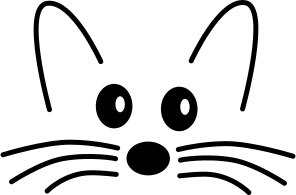
\includegraphics[width=1.4em]{squeak-logo}}}
\iftoshelse{
	\usepackage{marginnote}
		\renewcommand*{\marginfont}{\footnotesize}
	\newcommand{\vartriangleout}{\ifthenelse{\isodd{\thepage}}{\vartriangleright}{\vartriangleleft}}
	\newcommand{\dothisicon}{\fcolorbox{blue!65}{white}{\highlight{$\vartriangleout$}}}
	\newcommand{\dothis}[1]{%
		\noindent\par\noindent
		{\reversemarginpar
			\marginnote{\fcolorbox{blue!65}{white}{\highlight{$\vartriangleout$}}}}
		%\MarginLabel{do this}
		\noindent\emph{#1}
		\nopagebreak}
}{
	\newcommand{\dothisicon}{\raisebox{-.5ex}{
\includegraphics[height=1.2em]{pharo}}}
	\newcommand{\dothis}[1]{%
		\medskip
		\noindent\dothisicon
		\ifx#1\empty\else\quad\emph{#1}\fi
		\par\smallskip\nopagebreak}
}
%===> NEW VERSION <===
% NB: To use this in an individual chapter, you must set:
%\graphicspath{{figures/} {../figures/}}
% at the head of the chapter.  Don't forget the final /
%=============================================================
%:Reader hints (hint)
%
% Indicates a non-obvious consequence 
\newcommand{\hint}[1]{\vspace{1ex}\noindent\fbox{\textsc{Hint}} \emph{#1}}
%=================================================================
% graphics for Morphic handles
\newcommand{\grabHandle}{\raisebox{-0.2ex}{
\includegraphics[width=1em]{blackHandle}}}
\newcommand{\moveHandle}{\raisebox{-0.2ex}{
\includegraphics[width=1em]{moveHandle}}}
\newcommand{\debugHandle}{\raisebox{-0.2ex}{
\includegraphics[width=1em]{debugHandle}}}
%=============================================================
%:Highlighting Important stuff (doublebox)
%
% From Seaside book ...
\newsavebox{\SavedText}
\newlength{\InnerBoxRule}\setlength{\InnerBoxRule}{.75\fboxrule}
\newlength{\OuterBoxRule}\setlength{\OuterBoxRule}{1.5\fboxrule}
\newlength{\BoxSeparation}\setlength{\BoxSeparation}{1.5\fboxrule}
\addtolength{\BoxSeparation}{.5pt}
\newlength{\SaveBoxSep}\setlength{\SaveBoxSep}{2\fboxsep}
%
\newenvironment{doublebox}{\begin{lrbox}{\SavedText}
    \begin{minipage}{.75\textwidth}}
    {\end{minipage}\end{lrbox}\begin{center}
    \setlength{\fboxsep}{\BoxSeparation}\setlength{\fboxrule}{\OuterBoxRule}
    \fbox{\setlength{\fboxsep}{\SaveBoxSep}\setlength{\fboxrule}{\InnerBoxRule}%
      \fbox{\usebox{\SavedText}}}
  \end{center}}
% Use this:
\newcommand{\important}[1]{\begin{doublebox}#1\end{doublebox}}
%=============================================================
%:Section depth
\setcounter{secnumdepth}{2}
%% for this to happen start the file with
%\ifx\wholebook\relax\else
%% $Author$
% $Date$
% $Revision$

% HISTORY:
% 2006-10-31 - Oscar code macros
% ...

%=============================================================
% NB: documentclass must be set in main document.
% Allows book to be generated in multiple formats.
%=============================================================
%:Packages
\usepackage[T1]{fontenc}  %%%%%% really important to get the code directly in the text!
\usepackage{lmodern}
%\usepackage[scaled=0.85]{bookmanx} % needs another scale factor if used with \renewcommand{\sfdefault}{cmbr}
\usepackage{palatino}
\usepackage[scaled=0.85]{helvet}
\usepackage[protrusion,expansion=false]{microtype}
\usepackage{graphicx}
\usepackage{theorem}
\usepackage[english]{babel}
% ON: pdfsync breaks the use of p{width} for tabular columns!
\ifdefined\usepdfsync\usepackage{pdfsync}\fi % Requires texlive 2007
%=============================================================
%:More packages
%Stef should check which ones are used!
%\usepackage{picinpar}
%\usepackage{layout}
%\usepackage{color}
%\usepackage{enum}
%\usepackage{a4wide}
% \usepackage{fancyhdr}
\usepackage{ifthen}
\usepackage{float}
\usepackage{longtable}
\usepackage{makeidx}
\usepackage[nottoc]{tocbibind}
\usepackage{multicol}
\usepackage{booktabs}	% book-style tables
\usepackage{topcapt}	% enables \topcaption
\usepackage{multirow}
\usepackage{tabularx}
%\usepackage[bottom]{footmisc}
\usepackage{xspace}
\usepackage{alltt}
\usepackage{amssymb,textcomp}
\usepackage[usenames,dvipsnames]{color}
%\usepackage{colortbl}
\usepackage[hang]{subfigure}\makeatletter\def\p@subfigure{\thefigure\,}\makeatother
\usepackage{rotating}
\usepackage{enumitem}	% apb: allows more control over tags in enumerations
\usepackage{verbatim}     % for comment environment
\usepackage{varioref}	% for page references that work
\labelformat{footnote}{\thechapter--#1} % to distinguish citations from jurabib
\usepackage{needspace}
\usepackage{isodateo} % enable \isodate
\usepackage[newparttoc]{titlesec}
\usepackage{titletoc}
\usepackage{wrapfig}
\usepackage[
	super,
	citefull=first,
	authorformat={allreversed,and},
	titleformat={commasep,italic}
]{jurabib} % citations as footnotes
\usepackage[
	colorlinks=true,
	linkcolor=black,
	urlcolor=black,
	citecolor=black
]{hyperref}   % should come last
%=============================================================
%:PDF version
\pdfminorversion=3 % Set PDF to 1.3 for Lulu
%=============================================================
%:URL style
\makeatletter
\def\url@leostyle{%
  \@ifundefined{selectfont}{\def\UrlFont{\sf}}{\def\UrlFont{\sffamily}}}
\makeatother
% Now actually use the newly defined style.
\urlstyle{leo}
%=============================================================
%:Booleans
\newboolean{lulu}
\setboolean{lulu}{false}
\newcommand{\ifluluelse}[2]{\ifthenelse{\boolean{lulu}}{#1}{#2}}
%=============================================================
%:Names
\newcommand{\SUnit}{SUnit\xspace}
\newcommand{\sunit}{SUnit\xspace}
\newcommand{\xUnit}{$x$Unit\xspace}
\newcommand{\JUnit}{JUnit\xspace}
\newcommand{\st}{Smalltalk\xspace}
\newcommand{\pharo}{Pharo\xspace} % Use this, not \Pharo
%\newcommand{\sqmap}{SqueakMap\xspace}
\newcommand{\squeak}{Squeak\xspace} % use this, not \Squeak or \sq
\newcommand{\sqsrc}{SqueakSource\xspace}
\newcommand{\sbe}{\url{http://SqueakByExample.org}\xspace}
\newcommand{\pharoweb}{\url{http://pharo-project.org}\xspace}
\newcommand{\pbe}{\url{http://PharoByExample.org}\xspace}
\newcommand{\sba}{\url{http://SquareBracketAssociates.org}\xspace}
\newcommand{\bam}{\lct{Bounc\-ing\-Atoms\-Morph}\xspace}
%=============================================================
%:Markup macros for proof-reading
\usepackage[normalem]{ulem} % for \sout
\usepackage{xcolor}
\newcommand{\ra}{$\rightarrow$}
\newcommand{\ugh}[1]{\textcolor{red}{\uwave{#1}}} % please rephrase
\newcommand{\ins}[1]{\textcolor{blue}{\uline{#1}}} % please insert
\newcommand{\del}[1]{\textcolor{red}{\sout{#1}}} % please delete
\newcommand{\chg}[2]{\textcolor{red}{\sout{#1}}{\ra}\textcolor{blue}{\uline{#2}}} % please change
%=============================================================
%:Editorial comment macros
%\newcommand{\nnbb}[2]{
%    % \fbox{\bfseries\sffamily\scriptsize#1}
%    \fcolorbox{gray}{yellow}{\bfseries\sffamily\scriptsize#1}
%    {\sf\small$\blacktriangleright$\textit{#2}$\blacktriangleleft$}
%   }
\newcommand{\yellowbox}[1]{\fcolorbox{gray}{yellow}{\bfseries\sffamily\scriptsize#1}}
\newcommand{\triangles}[1]{{\sf\small$\blacktriangleright$\textit{#1}$\blacktriangleleft$}}
\newcommand{\nnbb}[2]{\yellowbox{#1} \triangles{#2}}
\newcommand{\fix}{\yellowbox{FIX!}}
\newcommand{\here}{\yellowbox{CONTINUE HERE!}}
% editor macros
\newcommand{\apl}[1]{\nnbb{Alain}{#1}} % Alain
\newcommand{\ab}[1]{\nnbb{Andrew}{#1}} % Black
\newcommand{\sd}[1]{\nnbb{St\'{e}f}{#1}} % Ducasse
\newcommand{\dc}[1]{\nnbb{DamienC}{#1}} % Ducasse
\newcommand{\md}[1]{\nnbb{Marcus}{#1}} % Denker
\newcommand{\on}[1]{\nnbb{Oscar}{#1}} % Nierstrasz
\newcommand{\damien}[1]{\nnbb{Damien}{#1}} % Pollet
\newcommand{\lr}[1]{\nnbb{Lukas}{#1}} % Renggli
\newcommand{\orla}[1]{\nnbb{Orla}{#1}} % Greevy
\newcommand{\alex}[1]{\nnbb{Alex}{#1}} % Bergel
\newcommand{\alx}[1]{\nnbb{Alex}{#1}} % Bergel
\newcommand{\dr}[1]{\nnbb{David}{#1}} % Roethlisberger
\newcommand{\ja}[1]{\nnbb{Jannik}{#1}} % Laval
\newcommand{\jr}[1]{\nnbb{Jorge}{#1}} % Ressia
\newcommand{\jb}[1]{\nnbb{JB}{#1}} % JB
\newcommand{\fp}[1]{\nnbb{Fabrizio}{#1}} % Perin
\newcommand{\michael}[1]{\nnbb{Michael}{#1}} % Davies
\newcommand{\ew}[1]{\nnbb{Erwann}{#1}} % Wernli
\newcommand{\mb}[1]{\nnbb{Martial}{#1}} % Boniou
\newcommand{\hw}[1]{\nnbb{Hernan}{#1}} % Wilkinson
\newcommand{\ben}[1]{\nnbb{Benjamin}{#1}} % Benjamin Van Ryseghem
%=============================================================
%:Abbreviation macros
\newcommand{\ie}{\emph{i.e.},\xspace}
\newcommand{\eg}{\emph{e.g.},\xspace}
\newcommand{\etc}{etc.\xspace}
%=============================================================
%:Cross reference macros
\newcommand{\charef}[1]{Chapter~\ref{cha:#1}\xspace}
\newcommand{\secref}[1]{Section~\ref{sec:#1}\xspace}
\newcommand{\figref}[1]{Figure~\ref{fig:#1}\xspace}
\newcommand{\Figref}[1]{Figure~\ref{fig:#1}\xspace}
\newcommand{\appref}[1]{Appendix~\ref{app:#1}\xspace}
\newcommand{\tabref}[1]{Table~\ref{tab:#1}\xspace}
\newcommand{\faqref}[1]{FAQ~\ref{faq:#1}, p.~\pageref{faq:#1}\xspace}
% APB: I removed trailing \xspace commands from these macros because
% \xspace mostly doesn't work.  If you want a space after your
% references, type one!
% ON: xspace has always worked just fine for me!  Please leave them in.
%
\newcommand{\ruleref}[1]{\ref{rule:#1}\xspace}
%
\newcommand{\egref}[1]{example~\ref{eg:#1}\xspace}
\newcommand{\Egref}[1]{Example~\ref{eg:#1}\xspace}
%
\newcommand{\scrref}[1]{script~\ref{scr:#1}\xspace}
\newcommand{\Scrref}[1]{Script~\ref{scr:#1}\xspace}
\newcommand{\tscrref}[1]{the script~\ref{scr:#1}\xspace}
\newcommand{\Tscrref}[1]{The script~\ref{scr:#1}\xspace}
%
\newcommand{\mthref}[1]{method~\ref{mth:#1}\xspace}
\newcommand{\mthsref}[1]{methods~\ref{mth:#1}\xspace}
\newcommand{\Mthref}[1]{Method~\ref{mth:#1}\xspace}
\newcommand{\tmthref}[1]{the method~\ref{mth:#1}\xspace}
\newcommand{\Tmthref}[1]{The method~\ref{mth:#1}\xspace}
%
\newcommand{\clsref}[1]{class~\ref{cls:#1}\xspace}
\newcommand{\tclsref}[1]{the class~\ref{cls:#1}\xspace}
\newcommand{\Tclsref}[1]{The class~\ref{cls:#1}\xspace}

\newcommand{\chalabel}[1]{\label{cha:#1}}
\newcommand{\seclabel}[1]{\label{sec:#1}}
\newcommand{\figlabel}[1]{\label{fig:#1}}
\newcommand{\tablabel}[1]{\label{tab:#1}}
\newcommand{\rulelabel}[1]{\label{rule:#1}}
\newcommand{\eglabel}[1]{\label{eg:#1}}
\newcommand{\scrlabel}[1]{\label{scr:#1}}
\newcommand{\mthlabel}[1]{\label{mth:#1}}
\newcommand{\clslabel}[1]{\label{cls:#1}}
\newcommand{\faqlabel}[1]{\label{faq:#1}}
%=============================================================
%:Menu item macro
% for menu items, so we can change our minds on how to print them! (apb)
\definecolor{lightgray}{gray}{0.89}
\newcommand{\menu}[1]{{%
	\setlength{\fboxsep}{0pt}%
	\colorbox{lightgray}{{{\upshape\sffamily\strut \,#1\,}}}}}
\newcommand{\link}[1]{{%
	\fontfamily{lmr}\selectfont
 	\upshape{\sffamily \underline{#1}}}}
% For submenu items:
\newcommand{\go}{\,$\triangleright$\,}
% \newcommand{\go}{\,$\blacktriangleright$\,}
% For keyboard shortcuts:
%\newcommand{\short}[1]{\mbox{$\langle${\sc CMD}$\rangle$-#1}\xspace}
\newcommand{\short}[1]{\mbox{{\sc cmd}\hspace{0.08em}--\hspace{0.09em}#1}\xspace}
% For buttons:
\newcommand{\button}[1]{{%
	\setlength{\fboxsep}{0pt}%
	\fbox{{\upshape\sffamily\strut \,#1\,}}}}
% NB: The button macro does not work within captions -- incompatible with xcolor package :-(
\newcommand{\toolsflap}{\textit{Tools} flap\xspace}
%=============================================================
%:Mouse clicks
\newcommand{\click}{click\xspace} % RED
\newcommand{\actclick}{action-click\xspace} % YELLOW
\newcommand{\metaclick}{meta-click\xspace} % BLUE
\newcommand{\Click}{Click\xspace} % RED
\newcommand{\Actclick}{Action-click\xspace} % YELLOW
\newcommand{\Metaclick}{Meta-click\xspace} % BLUE
%=============================================================
%:ToSh macros
\newboolean{tosh}
\setboolean{tosh}{false}
\newcommand{\iftoshelse}[2]{\ifthenelse{\boolean{tosh}}{#1}{#2}}
%=============================================================
%:ToSh colors
%\newcommand{\highlightcolor}{\color{blue!65}}
%\newcommand{\boxcolor}{\color{gray!25}}
\newcommand{\highlight}[1]{\textcolor{blue!65}{#1}}
%\newcommand{\codecolor}{\color{blue!65}}
%%\setlength{\fboxrule}{2pt}
%\newcommand{\asPict}[1]{%
%	{\Large\highlight{#1}}}
%=============================================================
%:Reader cues (do this)
%
% Indicate something the reader should try out.
% \newcommand{\dothisicon}{\raisebox{-.5ex}{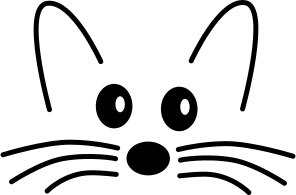
\includegraphics[width=1.4em]{squeak-logo}}}
\iftoshelse{
	\usepackage{marginnote}
		\renewcommand*{\marginfont}{\footnotesize}
	\newcommand{\vartriangleout}{\ifthenelse{\isodd{\thepage}}{\vartriangleright}{\vartriangleleft}}
	\newcommand{\dothisicon}{\fcolorbox{blue!65}{white}{\highlight{$\vartriangleout$}}}
	\newcommand{\dothis}[1]{%
		\noindent\par\noindent
		{\reversemarginpar
			\marginnote{\fcolorbox{blue!65}{white}{\highlight{$\vartriangleout$}}}}
		%\MarginLabel{do this}
		\noindent\emph{#1}
		\nopagebreak}
}{
	\newcommand{\dothisicon}{\raisebox{-.5ex}{
\includegraphics[height=1.2em]{pharo}}}
	\newcommand{\dothis}[1]{%
		\medskip
		\noindent\dothisicon
		\ifx#1\empty\else\quad\emph{#1}\fi
		\par\smallskip\nopagebreak}
}
%===> NEW VERSION <===
% NB: To use this in an individual chapter, you must set:
%\graphicspath{{figures/} {../figures/}}
% at the head of the chapter.  Don't forget the final /
%=============================================================
%:Reader hints (hint)
%
% Indicates a non-obvious consequence 
\newcommand{\hint}[1]{\vspace{1ex}\noindent\fbox{\textsc{Hint}} \emph{#1}}
%=================================================================
% graphics for Morphic handles
\newcommand{\grabHandle}{\raisebox{-0.2ex}{
\includegraphics[width=1em]{blackHandle}}}
\newcommand{\moveHandle}{\raisebox{-0.2ex}{
\includegraphics[width=1em]{moveHandle}}}
\newcommand{\debugHandle}{\raisebox{-0.2ex}{
\includegraphics[width=1em]{debugHandle}}}
%=============================================================
%:Highlighting Important stuff (doublebox)
%
% From Seaside book ...
\newsavebox{\SavedText}
\newlength{\InnerBoxRule}\setlength{\InnerBoxRule}{.75\fboxrule}
\newlength{\OuterBoxRule}\setlength{\OuterBoxRule}{1.5\fboxrule}
\newlength{\BoxSeparation}\setlength{\BoxSeparation}{1.5\fboxrule}
\addtolength{\BoxSeparation}{.5pt}
\newlength{\SaveBoxSep}\setlength{\SaveBoxSep}{2\fboxsep}
%
\newenvironment{doublebox}{\begin{lrbox}{\SavedText}
    \begin{minipage}{.75\textwidth}}
    {\end{minipage}\end{lrbox}\begin{center}
    \setlength{\fboxsep}{\BoxSeparation}\setlength{\fboxrule}{\OuterBoxRule}
    \fbox{\setlength{\fboxsep}{\SaveBoxSep}\setlength{\fboxrule}{\InnerBoxRule}%
      \fbox{\usebox{\SavedText}}}
  \end{center}}
% Use this:
\newcommand{\important}[1]{\begin{doublebox}#1\end{doublebox}}
%=============================================================
%:Section depth
\setcounter{secnumdepth}{2}
%% for this to happen start the file with
%\ifx\wholebook\relax\else
%% $Author$
% $Date$
% $Revision$

% HISTORY:
% 2006-10-31 - Oscar code macros
% ...

%=============================================================
% NB: documentclass must be set in main document.
% Allows book to be generated in multiple formats.
%=============================================================
%:Packages
\usepackage[T1]{fontenc}  %%%%%% really important to get the code directly in the text!
\usepackage{lmodern}
%\usepackage[scaled=0.85]{bookmanx} % needs another scale factor if used with \renewcommand{\sfdefault}{cmbr}
\usepackage{palatino}
\usepackage[scaled=0.85]{helvet}
\usepackage[protrusion,expansion=false]{microtype}
\usepackage{graphicx}
\usepackage{theorem}
\usepackage[english]{babel}
% ON: pdfsync breaks the use of p{width} for tabular columns!
\ifdefined\usepdfsync\usepackage{pdfsync}\fi % Requires texlive 2007
%=============================================================
%:More packages
%Stef should check which ones are used!
%\usepackage{picinpar}
%\usepackage{layout}
%\usepackage{color}
%\usepackage{enum}
%\usepackage{a4wide}
% \usepackage{fancyhdr}
\usepackage{ifthen}
\usepackage{float}
\usepackage{longtable}
\usepackage{makeidx}
\usepackage[nottoc]{tocbibind}
\usepackage{multicol}
\usepackage{booktabs}	% book-style tables
\usepackage{topcapt}	% enables \topcaption
\usepackage{multirow}
\usepackage{tabularx}
%\usepackage[bottom]{footmisc}
\usepackage{xspace}
\usepackage{alltt}
\usepackage{amssymb,textcomp}
\usepackage[usenames,dvipsnames]{color}
%\usepackage{colortbl}
\usepackage[hang]{subfigure}\makeatletter\def\p@subfigure{\thefigure\,}\makeatother
\usepackage{rotating}
\usepackage{enumitem}	% apb: allows more control over tags in enumerations
\usepackage{verbatim}     % for comment environment
\usepackage{varioref}	% for page references that work
\labelformat{footnote}{\thechapter--#1} % to distinguish citations from jurabib
\usepackage{needspace}
\usepackage{isodateo} % enable \isodate
\usepackage[newparttoc]{titlesec}
\usepackage{titletoc}
\usepackage{wrapfig}
\usepackage[
	super,
	citefull=first,
	authorformat={allreversed,and},
	titleformat={commasep,italic}
]{jurabib} % citations as footnotes
\usepackage[
	colorlinks=true,
	linkcolor=black,
	urlcolor=black,
	citecolor=black
]{hyperref}   % should come last
%=============================================================
%:PDF version
\pdfminorversion=3 % Set PDF to 1.3 for Lulu
%=============================================================
%:URL style
\makeatletter
\def\url@leostyle{%
  \@ifundefined{selectfont}{\def\UrlFont{\sf}}{\def\UrlFont{\sffamily}}}
\makeatother
% Now actually use the newly defined style.
\urlstyle{leo}
%=============================================================
%:Booleans
\newboolean{lulu}
\setboolean{lulu}{false}
\newcommand{\ifluluelse}[2]{\ifthenelse{\boolean{lulu}}{#1}{#2}}
%=============================================================
%:Names
\newcommand{\SUnit}{SUnit\xspace}
\newcommand{\sunit}{SUnit\xspace}
\newcommand{\xUnit}{$x$Unit\xspace}
\newcommand{\JUnit}{JUnit\xspace}
\newcommand{\st}{Smalltalk\xspace}
\newcommand{\pharo}{Pharo\xspace} % Use this, not \Pharo
%\newcommand{\sqmap}{SqueakMap\xspace}
\newcommand{\squeak}{Squeak\xspace} % use this, not \Squeak or \sq
\newcommand{\sqsrc}{SqueakSource\xspace}
\newcommand{\sbe}{\url{http://SqueakByExample.org}\xspace}
\newcommand{\pharoweb}{\url{http://pharo-project.org}\xspace}
\newcommand{\pbe}{\url{http://PharoByExample.org}\xspace}
\newcommand{\sba}{\url{http://SquareBracketAssociates.org}\xspace}
\newcommand{\bam}{\lct{Bounc\-ing\-Atoms\-Morph}\xspace}
%=============================================================
%:Markup macros for proof-reading
\usepackage[normalem]{ulem} % for \sout
\usepackage{xcolor}
\newcommand{\ra}{$\rightarrow$}
\newcommand{\ugh}[1]{\textcolor{red}{\uwave{#1}}} % please rephrase
\newcommand{\ins}[1]{\textcolor{blue}{\uline{#1}}} % please insert
\newcommand{\del}[1]{\textcolor{red}{\sout{#1}}} % please delete
\newcommand{\chg}[2]{\textcolor{red}{\sout{#1}}{\ra}\textcolor{blue}{\uline{#2}}} % please change
%=============================================================
%:Editorial comment macros
%\newcommand{\nnbb}[2]{
%    % \fbox{\bfseries\sffamily\scriptsize#1}
%    \fcolorbox{gray}{yellow}{\bfseries\sffamily\scriptsize#1}
%    {\sf\small$\blacktriangleright$\textit{#2}$\blacktriangleleft$}
%   }
\newcommand{\yellowbox}[1]{\fcolorbox{gray}{yellow}{\bfseries\sffamily\scriptsize#1}}
\newcommand{\triangles}[1]{{\sf\small$\blacktriangleright$\textit{#1}$\blacktriangleleft$}}
\newcommand{\nnbb}[2]{\yellowbox{#1} \triangles{#2}}
\newcommand{\fix}{\yellowbox{FIX!}}
\newcommand{\here}{\yellowbox{CONTINUE HERE!}}
% editor macros
\newcommand{\apl}[1]{\nnbb{Alain}{#1}} % Alain
\newcommand{\ab}[1]{\nnbb{Andrew}{#1}} % Black
\newcommand{\sd}[1]{\nnbb{St\'{e}f}{#1}} % Ducasse
\newcommand{\dc}[1]{\nnbb{DamienC}{#1}} % Ducasse
\newcommand{\md}[1]{\nnbb{Marcus}{#1}} % Denker
\newcommand{\on}[1]{\nnbb{Oscar}{#1}} % Nierstrasz
\newcommand{\damien}[1]{\nnbb{Damien}{#1}} % Pollet
\newcommand{\lr}[1]{\nnbb{Lukas}{#1}} % Renggli
\newcommand{\orla}[1]{\nnbb{Orla}{#1}} % Greevy
\newcommand{\alex}[1]{\nnbb{Alex}{#1}} % Bergel
\newcommand{\alx}[1]{\nnbb{Alex}{#1}} % Bergel
\newcommand{\dr}[1]{\nnbb{David}{#1}} % Roethlisberger
\newcommand{\ja}[1]{\nnbb{Jannik}{#1}} % Laval
\newcommand{\jr}[1]{\nnbb{Jorge}{#1}} % Ressia
\newcommand{\jb}[1]{\nnbb{JB}{#1}} % JB
\newcommand{\fp}[1]{\nnbb{Fabrizio}{#1}} % Perin
\newcommand{\michael}[1]{\nnbb{Michael}{#1}} % Davies
\newcommand{\ew}[1]{\nnbb{Erwann}{#1}} % Wernli
\newcommand{\mb}[1]{\nnbb{Martial}{#1}} % Boniou
\newcommand{\hw}[1]{\nnbb{Hernan}{#1}} % Wilkinson
\newcommand{\ben}[1]{\nnbb{Benjamin}{#1}} % Benjamin Van Ryseghem
%=============================================================
%:Abbreviation macros
\newcommand{\ie}{\emph{i.e.},\xspace}
\newcommand{\eg}{\emph{e.g.},\xspace}
\newcommand{\etc}{etc.\xspace}
%=============================================================
%:Cross reference macros
\newcommand{\charef}[1]{Chapter~\ref{cha:#1}\xspace}
\newcommand{\secref}[1]{Section~\ref{sec:#1}\xspace}
\newcommand{\figref}[1]{Figure~\ref{fig:#1}\xspace}
\newcommand{\Figref}[1]{Figure~\ref{fig:#1}\xspace}
\newcommand{\appref}[1]{Appendix~\ref{app:#1}\xspace}
\newcommand{\tabref}[1]{Table~\ref{tab:#1}\xspace}
\newcommand{\faqref}[1]{FAQ~\ref{faq:#1}, p.~\pageref{faq:#1}\xspace}
% APB: I removed trailing \xspace commands from these macros because
% \xspace mostly doesn't work.  If you want a space after your
% references, type one!
% ON: xspace has always worked just fine for me!  Please leave them in.
%
\newcommand{\ruleref}[1]{\ref{rule:#1}\xspace}
%
\newcommand{\egref}[1]{example~\ref{eg:#1}\xspace}
\newcommand{\Egref}[1]{Example~\ref{eg:#1}\xspace}
%
\newcommand{\scrref}[1]{script~\ref{scr:#1}\xspace}
\newcommand{\Scrref}[1]{Script~\ref{scr:#1}\xspace}
\newcommand{\tscrref}[1]{the script~\ref{scr:#1}\xspace}
\newcommand{\Tscrref}[1]{The script~\ref{scr:#1}\xspace}
%
\newcommand{\mthref}[1]{method~\ref{mth:#1}\xspace}
\newcommand{\mthsref}[1]{methods~\ref{mth:#1}\xspace}
\newcommand{\Mthref}[1]{Method~\ref{mth:#1}\xspace}
\newcommand{\tmthref}[1]{the method~\ref{mth:#1}\xspace}
\newcommand{\Tmthref}[1]{The method~\ref{mth:#1}\xspace}
%
\newcommand{\clsref}[1]{class~\ref{cls:#1}\xspace}
\newcommand{\tclsref}[1]{the class~\ref{cls:#1}\xspace}
\newcommand{\Tclsref}[1]{The class~\ref{cls:#1}\xspace}

\newcommand{\chalabel}[1]{\label{cha:#1}}
\newcommand{\seclabel}[1]{\label{sec:#1}}
\newcommand{\figlabel}[1]{\label{fig:#1}}
\newcommand{\tablabel}[1]{\label{tab:#1}}
\newcommand{\rulelabel}[1]{\label{rule:#1}}
\newcommand{\eglabel}[1]{\label{eg:#1}}
\newcommand{\scrlabel}[1]{\label{scr:#1}}
\newcommand{\mthlabel}[1]{\label{mth:#1}}
\newcommand{\clslabel}[1]{\label{cls:#1}}
\newcommand{\faqlabel}[1]{\label{faq:#1}}
%=============================================================
%:Menu item macro
% for menu items, so we can change our minds on how to print them! (apb)
\definecolor{lightgray}{gray}{0.89}
\newcommand{\menu}[1]{{%
	\setlength{\fboxsep}{0pt}%
	\colorbox{lightgray}{{{\upshape\sffamily\strut \,#1\,}}}}}
\newcommand{\link}[1]{{%
	\fontfamily{lmr}\selectfont
 	\upshape{\sffamily \underline{#1}}}}
% For submenu items:
\newcommand{\go}{\,$\triangleright$\,}
% \newcommand{\go}{\,$\blacktriangleright$\,}
% For keyboard shortcuts:
%\newcommand{\short}[1]{\mbox{$\langle${\sc CMD}$\rangle$-#1}\xspace}
\newcommand{\short}[1]{\mbox{{\sc cmd}\hspace{0.08em}--\hspace{0.09em}#1}\xspace}
% For buttons:
\newcommand{\button}[1]{{%
	\setlength{\fboxsep}{0pt}%
	\fbox{{\upshape\sffamily\strut \,#1\,}}}}
% NB: The button macro does not work within captions -- incompatible with xcolor package :-(
\newcommand{\toolsflap}{\textit{Tools} flap\xspace}
%=============================================================
%:Mouse clicks
\newcommand{\click}{click\xspace} % RED
\newcommand{\actclick}{action-click\xspace} % YELLOW
\newcommand{\metaclick}{meta-click\xspace} % BLUE
\newcommand{\Click}{Click\xspace} % RED
\newcommand{\Actclick}{Action-click\xspace} % YELLOW
\newcommand{\Metaclick}{Meta-click\xspace} % BLUE
%=============================================================
%:ToSh macros
\newboolean{tosh}
\setboolean{tosh}{false}
\newcommand{\iftoshelse}[2]{\ifthenelse{\boolean{tosh}}{#1}{#2}}
%=============================================================
%:ToSh colors
%\newcommand{\highlightcolor}{\color{blue!65}}
%\newcommand{\boxcolor}{\color{gray!25}}
\newcommand{\highlight}[1]{\textcolor{blue!65}{#1}}
%\newcommand{\codecolor}{\color{blue!65}}
%%\setlength{\fboxrule}{2pt}
%\newcommand{\asPict}[1]{%
%	{\Large\highlight{#1}}}
%=============================================================
%:Reader cues (do this)
%
% Indicate something the reader should try out.
% \newcommand{\dothisicon}{\raisebox{-.5ex}{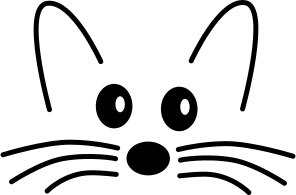
\includegraphics[width=1.4em]{squeak-logo}}}
\iftoshelse{
	\usepackage{marginnote}
		\renewcommand*{\marginfont}{\footnotesize}
	\newcommand{\vartriangleout}{\ifthenelse{\isodd{\thepage}}{\vartriangleright}{\vartriangleleft}}
	\newcommand{\dothisicon}{\fcolorbox{blue!65}{white}{\highlight{$\vartriangleout$}}}
	\newcommand{\dothis}[1]{%
		\noindent\par\noindent
		{\reversemarginpar
			\marginnote{\fcolorbox{blue!65}{white}{\highlight{$\vartriangleout$}}}}
		%\MarginLabel{do this}
		\noindent\emph{#1}
		\nopagebreak}
}{
	\newcommand{\dothisicon}{\raisebox{-.5ex}{
\includegraphics[height=1.2em]{pharo}}}
	\newcommand{\dothis}[1]{%
		\medskip
		\noindent\dothisicon
		\ifx#1\empty\else\quad\emph{#1}\fi
		\par\smallskip\nopagebreak}
}
%===> NEW VERSION <===
% NB: To use this in an individual chapter, you must set:
%\graphicspath{{figures/} {../figures/}}
% at the head of the chapter.  Don't forget the final /
%=============================================================
%:Reader hints (hint)
%
% Indicates a non-obvious consequence 
\newcommand{\hint}[1]{\vspace{1ex}\noindent\fbox{\textsc{Hint}} \emph{#1}}
%=================================================================
% graphics for Morphic handles
\newcommand{\grabHandle}{\raisebox{-0.2ex}{
\includegraphics[width=1em]{blackHandle}}}
\newcommand{\moveHandle}{\raisebox{-0.2ex}{
\includegraphics[width=1em]{moveHandle}}}
\newcommand{\debugHandle}{\raisebox{-0.2ex}{
\includegraphics[width=1em]{debugHandle}}}
%=============================================================
%:Highlighting Important stuff (doublebox)
%
% From Seaside book ...
\newsavebox{\SavedText}
\newlength{\InnerBoxRule}\setlength{\InnerBoxRule}{.75\fboxrule}
\newlength{\OuterBoxRule}\setlength{\OuterBoxRule}{1.5\fboxrule}
\newlength{\BoxSeparation}\setlength{\BoxSeparation}{1.5\fboxrule}
\addtolength{\BoxSeparation}{.5pt}
\newlength{\SaveBoxSep}\setlength{\SaveBoxSep}{2\fboxsep}
%
\newenvironment{doublebox}{\begin{lrbox}{\SavedText}
    \begin{minipage}{.75\textwidth}}
    {\end{minipage}\end{lrbox}\begin{center}
    \setlength{\fboxsep}{\BoxSeparation}\setlength{\fboxrule}{\OuterBoxRule}
    \fbox{\setlength{\fboxsep}{\SaveBoxSep}\setlength{\fboxrule}{\InnerBoxRule}%
      \fbox{\usebox{\SavedText}}}
  \end{center}}
% Use this:
\newcommand{\important}[1]{\begin{doublebox}#1\end{doublebox}}
%=============================================================
%:Section depth
\setcounter{secnumdepth}{2}
%% for this to happen start the file with
%\ifx\wholebook\relax\else
%\input{../common.tex}
%\begin{document}
%\fi
% and terminate by
% \ifx\wholebook\relax\else\end{document}\fi

\DeclareGraphicsExtensions{.pdf, .jpg, .png}
%=============================================================
%:PDF setup
\hypersetup{
%   a4paper,
%   pdfstartview=FitV,
%   colorlinks,
%   linkcolor=darkblue,
%   citecolor=darkblue,
   pdftitle={Pharo by Example},
   pdfauthor={Andrew P. Black, St\'ephane Ducasse,	Oscar Nierstrasz,
Damien Pollet},
   pdfkeywords={Smalltalk, Squeak, Object-Oriented Programming, OOP},
   pdfsubject={Computer Science}
}
%=============================================================
%:Page layout and appearance
%
% \renewcommand{\headrulewidth}{0pt}
\renewcommand{\chaptermark}[1]{\markboth{#1}{}}
\renewcommand{\sectionmark}[1]{\markright{\thesection\ #1}}
\renewpagestyle{plain}[\small\itshape]{%
	\setheadrule{0pt}%
	\sethead[][][]{}{}{}%
	\setfoot[][][]{}{}{}}
\renewpagestyle{headings}[\small\itshape]{%
	\setheadrule{0pt}%
	\setmarks{chapter}{section}%
	\sethead[\thepage][][\chaptertitle]{\sectiontitle}{}{\thepage}%
	\setfoot[][][]{}{}{}}
%=============================================================
%:Title section setup and TOC numbering depth
\setcounter{secnumdepth}{1}
\setcounter{tocdepth}{1}
\titleformat{\part}[display]{\centering}{\huge\partname\ \thepart}{1em}{\Huge\textbf}[]
\titleformat{\chapter}[display]{}{\huge\chaptertitlename\ \thechapter}{1em}{\Huge\raggedright\textbf}[]
\titlecontents{part}[3pc]{%
		\pagebreak[2]\addvspace{1em plus.4em minus.2em}%
		\leavevmode\large\bfseries}
	{\contentslabel{3pc}}{\hspace*{-3pc}}
	{}[\nopagebreak]
\titlecontents{chapter}[3pc]{%
		\pagebreak[0]\addvspace{1em plus.2em minus.2em}%
		\leavevmode\bfseries}
	{\contentslabel{3pc}}{}
	{\hfill\contentspage}[\nopagebreak]
\dottedcontents{section}[3pc]{}{3pc}{1pc}
\dottedcontents{subsection}[3pc]{}{0pc}{1pc}
% \dottedcontents{subsection}[4.5em]{}{0pt}{1pc}
% Make \cleardoublepage insert really blank pages http://www.tex.ac.uk/cgi-bin/texfaq2html?label=reallyblank
\let\origdoublepage\cleardoublepage
\newcommand{\clearemptydoublepage}{%
  \clearpage
  {\pagestyle{empty}\origdoublepage}}
\let\cleardoublepage\clearemptydoublepage % see http://www.tex.ac.uk/cgi-bin/texfaq2html?label=patch
%=============================================================
%:FAQ macros (for FAQ chapter)
\newtheorem{faq}{FAQ}
\newcommand{\answer}{\paragraph{Answer}\ }
%=============================================================
%:Listings package configuration
% \newcommand{\caret}{\makebox{\raisebox{0.4ex}{\footnotesize{$\wedge$}}}}
\newcommand{\caret}{\^\,}
\newcommand{\escape}{{\sf \textbackslash}}
\definecolor{source}{gray}{0.95}
\usepackage{listings}
\lstdefinelanguage{Smalltalk}{
%  morekeywords={self,super,true,false,nil,thisContext}, % This is overkill
  morestring=[d]',
  morecomment=[s]{"}{"},
  alsoletter={\#:},
  escapechar={!},
  literate=
    {BANG}{!}1
    {CARET}{\^}1
    {UNDERSCORE}{\_}1
    {\\st}{Smalltalk}9 % convenience -- in case \st occurs in code
    % {'}{{\textquotesingle}}1 % replaced by upquote=true in \lstset
    {_}{{$\leftarrow$}}1
    {>>>}{{\sep}}1
    {^}{{$\uparrow$}}1
    {~}{{$\sim$}}1
    {-}{{\texttt{-}}}1 %{\textminus}}1 %{-}{\hspace{-0.13em}}{-}}1  % the goal is to make - the same width as +
    % {+}{\sf+}1 %{\raisebox{0.08ex}{+}}}1      % and to raise + off the baseline to match -
    {-->}{{\quad$\longrightarrow$\quad}}3
	, % Don't forget the comma at the end!
  tabsize=4
}[keywords,comments,strings]

\lstset{language=Smalltalk,
	basicstyle=\sffamily,
	keywordstyle=\color{black}\bfseries,
	% stringstyle=\ttfamily, % Ugly! do we really want this? -- on
	mathescape=true,
	showstringspaces=false,
	keepspaces=true,
	breaklines=true,
	breakautoindent=true,
	backgroundcolor=\color{source},
	lineskip={-1pt}, % Ugly hack
	upquote=true, % straight quote; requires textcomp package
	columns=fullflexible} % no fixed width fonts
% In-line code (literal)
% Normally use this for all in-line code:
\newcommand{\ct}{\lstinline[mathescape=false,backgroundcolor=\color{white},basicstyle={\sffamily\upshape}]}
% apb 2007.8.28 added the \upshape declaration to avoid getting italicized code in \dothis{ } sections.
% In-line code (latex enabled)
% Use this only in special situations where \ct does not work
% (within section headings ...):
\newcommand{\lct}[1]{{\textsf{\textup{#1}}}}
% Use these for system categories and protocols:
\newcommand{\scat}[1]{\emph{\textsf{#1}}\xspace}
\newcommand{\pkg}[1]{\emph{\textsf{#1}}\xspace}
\newcommand{\prot}[1]{\emph{\textsf{#1}}\xspace}
% Code environments
% NB: the arg is for tests
% Only code and example environments may be tests
\lstnewenvironment{code}[1]{%
	\lstset{%
		% frame=lines,
		frame=single,
		framerule=0pt,
		mathescape=false
	}
}{}
\def\ignoredollar#1{}
%=============================================================
%:Code environments (method, script ...)
% NB: the third arg is for tests
% Only code and example environments may be tests
\lstnewenvironment{example}[3][defaultlabel]{%
	\renewcommand{\lstlistingname}{Example}%
	\lstset{
		% frame=lines,
		frame=single,
		framerule=0pt,
		mathescape=false,
		caption={\emph{#2}},
		label={eg:#1}
	}
}{}
\lstnewenvironment{script}[2][defaultlabel]{%
\renewcommand{\lstlistingname}{Script}%
	\lstset{
		% frame=lines,
		frame=single,
		framerule=0pt,
		mathescape=false,
		name={Script},
		caption={\emph{#2}},
		label={scr:#1}
	}
}{}
\lstnewenvironment{method}[2][defaultlabel]{%
	\renewcommand{\lstlistingname}{Method}%
	\lstset{
		% frame=lines,
		frame=single,
		framerule=0pt,
		mathescape=false,
		name={Method},
		caption={\emph{#2}},
		label={mth:#1}
	}
}{}
\lstnewenvironment{methods}[2][defaultlabel]{% just for multiple methods at once
	\renewcommand{\lstlistingname}{Methods}%
	\lstset{
		% frame=lines,
		frame=single,
		framerule=0pt,
		mathescape=false,
		name={Method},
		caption={\emph{#2}},
		label={mth:#1}
	}
}{}
\lstnewenvironment{numMethod}[2][defaultlabel]{%
	\renewcommand{\lstlistingname}{Method}%
	\lstset{
		numbers=left,
		numberstyle={\tiny\sffamily},
		% frame=lines,
		frame=single,
		framerule=0pt,
		mathescape=false,
		name={Method},
		caption={\emph{#2}},
		label={mth:#1}
	}
}{}
\lstnewenvironment{classdef}[2][defaultlabel]{%
	\renewcommand{\lstlistingname}{Class}%
	\lstset{
		% frame=lines,
		frame=single,
		framerule=0pt,
		mathescape=false,
		name={Class},
		caption={\emph{#2}},
		label={cls:#1}
	}
}{}
%=============================================================
%:Reserving space
% Usually need one more line than the actual lines of code
\newcommand{\needlines}[1]{\Needspace{#1\baselineskip}}
%=============================================================
%:Indexing macros
% Macros ending with "ind" generate text as well as an index entry
% Macros ending with "index" *only* generate an index entry
\newcommand{\ind}[1]{\index{#1}#1\xspace} % plain text
\newcommand{\subind}[2]{\index{#1!#2}#2\xspace} % show #2, subindex under #1
\newcommand{\emphind}[1]{\index{#1}\emph{#1}\xspace} % emph #1
\newcommand{\emphsubind}[2]{\index{#1!#2}\emph{#2}\xspace} % show emph #2, subindex inder #1
\newcommand{\scatind}[1]{\index{#1@\textsf{#1} (category)}\scat{#1}} % category
\newcommand{\pkgind}[1]{\index{#1@\textsf{#1} (package)}\pkg{#1}} % package
\newcommand{\protind}[1]{\index{#1@\textsf{#1} (protocol)}\prot{#1}} % protocol
\newcommand{\clsind}[1]{\index{#1@\textsf{#1} (class)}\ct{#1}\xspace}
% \newcommand{\clsind}[1]{\index{#1!\#@(class)}\ct{#1}\xspace} % class
\newcommand{\clsindplural}[1]{\index{#1!\#@(class)}\ct{#1}s\xspace} % class
\newcommand{\cvind}[1]{\index{#1@\textsf{#1} (class variable)}\ct{#1}\xspace} % class var
\newcommand{\glbind}[1]{\index{#1@\textsf{#1} (global)}\ct{#1}\xspace} % global
\newcommand{\patind}[1]{\index{#1@#1 (pattern)}\ct{#1}\xspace} % pattern
\newcommand{\pvind}[1]{\index{#1@\textsf{#1} (pseudo variable)}\ct{#1}\xspace} % pseudo var
\newcommand{\clsmthind}[2]{\index{#1!#2@\ct{#2}}\ct{#1>>>#2}\xspace} % class + method name
\newcommand{\mthind}[2]{\index{#1!#2@\ct{#2}}\ct{#2}\xspace} % show method name only
\newcommand{\lmthind}[2]{\index{#1!#2@\ct{#2}}\lct{#2}\xspace} % show method name only
\newcommand{\cmind}[2]{\index{#1!#2@\ct{#2}}\ct{#1>>>#2}\xspace} % show class>>method
\newcommand{\lcmind}[2]{\index{#1!#2@\ct{#2}}\lct{#1>>>#2}\xspace} % show class>>method
\newcommand{\toolsflapind}{\index{Tools flap}\toolsflap} % index tools flap
% The following only generate an index entry:
% \newcommand{\clsindex}[1]{\index{#1@\textsf{#1} (class)}}
\newcommand{\clsindex}[1]{\index{#1!\#@(class)}} % class
\newcommand{\mthindex}[2]{\index{#1!#2@\ct{#2}}} % method
\newcommand{\cmindex}[2]{\index{#1!#2@\ct{#2}}} % class>>method
\newcommand{\cvindex}[1]{\index{#1@\textsf{#1} (class variable)}} % class var
\newcommand{\glbindex}[1]{\index{#1@\textsf{#1} (global)}}% global
\newcommand{\pvindex}[1]{\index{#1@\textsf{#1} (pseudo variable)}}% pseudo var
\newcommand{\seeindex}[2]{\index{#1|see{#2}}} % #1, see #2
\newcommand{\scatindex}[1]{\index{#1@\textsf{#1} (category)}} % category
\newcommand{\pkgindex}[1]{\index{#1@\textsf{#1} (package)}} % package
\newcommand{\protindex}[1]{\index{#1@\textsf{#1} (protocol)}} % protocol
% How can we have the main entry page numbers in bold yet not break the hyperlink?
\newcommand{\boldidx}[1]{{\bf #1}} % breaks hyperlink
%\newcommand{\indmain}[1]{\index{#1|boldidx}#1\xspace} % plain text, main entry
%\newcommand{\emphsubindmain}[2]{\index{#1!#2|boldidx}\emph{#2}\xspace} % subindex, main entry
%\newcommand{\subindmain}[2]{\index{#1!#2|boldidx}#2\xspace} % subindex, main entry
%\newcommand{\clsindmain}[1]{\index{#1@\textsf{#1} (class)|boldidx}\ct{#1}\xspace}
%\newcommand{\clsindmain}[1]{\index{#1!\#@(class)|boldidx}\ct{#1}\xspace} % class main
%\newcommand{\indexmain}[1]{\index{#1|boldidx}} % main index entry only
\newcommand{\indmain}[1]{\index{#1}#1\xspace} % The main index entry for this item
\newcommand{\emphsubindmain}[2]{\index{#1!#2}\emph{#2}\xspace} % subindex, main entry
\newcommand{\subindmain}[2]{\index{#1!#2}#2\xspace} % subindex, main entry
%\newcommand{\clsindmain}[1]{\index{#1@\textsf{#1} (class)}\ct{#1}\xspace}
\newcommand{\clsindmain}[1]{\index{#1!\#@(class)}\ct{#1}\xspace} % class main
\newcommand{\clsindexmain}[1]{\index{#1!\#@(class)}} % class main index only
\newcommand{\indexmain}[1]{\index{#1}} 
%=============================================================
%:Code macros
% some constants
\newcommand{\codesize}{\small}
\newcommand{\codefont}{\sffamily}
%\newcommand{\cat}[1]{\textit{In category #1}}%%To remove later
\newlength{\scriptindent}
\setlength{\scriptindent}{.3cm}
%% Method presentation constants
\newlength{\methodindent}
\newlength{\methodwordlength}
\newlength{\aftermethod}
\setlength{\methodindent}{0.2cm}
\settowidth{\methodwordlength}{\ M\'ethode\ }
%=============================================================
%:Smalltalk macros
%\newcommand{\sep}{{$\gg$}}
\newcommand{\sep}{\mbox{>>}}
\newcommand{\self}{\lct{self}\xspace}
\newcommand{\super}{\lct{super}\xspace}
\newcommand{\nil}{\lct{nil}\xspace}
%=============================================================
% be less conservative about float placement
% these commands are from http://www.tex.ac.uk/cgi-bin/texfaq2html?label=floats
\renewcommand{\topfraction}{.9}
\renewcommand{\bottomfraction}{.9}
\renewcommand{\textfraction}{.1}
\renewcommand{\floatpagefraction}{.85}
\renewcommand{\dbltopfraction}{.66}
\renewcommand{\dblfloatpagefraction}{.85}
\setcounter{topnumber}{9}
\setcounter{bottomnumber}{9}
\setcounter{totalnumber}{20}
\setcounter{dbltopnumber}{9}
%=============================================================
% Give information from each chapter's author
\newcommand{\contact}[2]{\textbf{#1} \textsf{(#2)}}

\newcommand{\chapterauthor}[1]{\emph{with the participation of:\\#1}\\}

\newcommand{\authornoury}{\contact{Noury Bouraqadi}{bouraqadi@gmail.com}}
\newcommand{\authordamienc}{\contact{Damien Cassou}{damien.cassou@gmail.com}}
\newcommand{\authoroscar}{\contact{Oscar Nierstrasz}{oscar.nierstrasz@acm.org}}
\newcommand{\authorsteph}{\contact{St\'ephane Ducasse}{stephane.ducasse@inria.fr}}
\newcommand{\authoralex}{\contact{Alexandre Bergel}{alexandre@bergel.eu}}
\newcommand{\authorolivier}{\contact{Olivier Auverlot}{olivier.auverlot@inria.fr}}
\newcommand{\authornicolas}{\contact{Nicolas Cellier}{nicolas.cellier.aka.nice@gmail.com}}
\newcommand{\authormarcus}{\contact{Marcus Denker}{marcus.denker@inria.fr}}
\newcommand{\authoralain}{\contact{Alain Plantec}{alain.plantec@univ-brest.fr}}
\newcommand{\authordale}{\contact{Dale Henrichs}{dale.henrichs@gemstone.com}}
\newcommand{\authormariano}{\contact{Mariano Martinez Peck}{marianopeck@gmail.com}}
\newcommand{\authorsven}{\contact{Sven Van Caekenberghe}{sven@beta9.be}}
\newcommand{\authorlukas}{\contact{Lukas Renggli}{renggli@gmail.com}}

%=============================================================
% apb doesn't like paragraphs to run in to each other without a break
\parskip 1ex
%=============================================================
%:Stuff to check, merge or deprecate
%\setlength{\marginparsep}{2mm}
%\renewcommand{\baselinestretch}{1.1}
%=============================================================

%\begin{document}
%\fi
% and terminate by
% \ifx\wholebook\relax\else\end{document}\fi

\DeclareGraphicsExtensions{.pdf, .jpg, .png}
%=============================================================
%:PDF setup
\hypersetup{
%   a4paper,
%   pdfstartview=FitV,
%   colorlinks,
%   linkcolor=darkblue,
%   citecolor=darkblue,
   pdftitle={Pharo by Example},
   pdfauthor={Andrew P. Black, St\'ephane Ducasse,	Oscar Nierstrasz,
Damien Pollet},
   pdfkeywords={Smalltalk, Squeak, Object-Oriented Programming, OOP},
   pdfsubject={Computer Science}
}
%=============================================================
%:Page layout and appearance
%
% \renewcommand{\headrulewidth}{0pt}
\renewcommand{\chaptermark}[1]{\markboth{#1}{}}
\renewcommand{\sectionmark}[1]{\markright{\thesection\ #1}}
\renewpagestyle{plain}[\small\itshape]{%
	\setheadrule{0pt}%
	\sethead[][][]{}{}{}%
	\setfoot[][][]{}{}{}}
\renewpagestyle{headings}[\small\itshape]{%
	\setheadrule{0pt}%
	\setmarks{chapter}{section}%
	\sethead[\thepage][][\chaptertitle]{\sectiontitle}{}{\thepage}%
	\setfoot[][][]{}{}{}}
%=============================================================
%:Title section setup and TOC numbering depth
\setcounter{secnumdepth}{1}
\setcounter{tocdepth}{1}
\titleformat{\part}[display]{\centering}{\huge\partname\ \thepart}{1em}{\Huge\textbf}[]
\titleformat{\chapter}[display]{}{\huge\chaptertitlename\ \thechapter}{1em}{\Huge\raggedright\textbf}[]
\titlecontents{part}[3pc]{%
		\pagebreak[2]\addvspace{1em plus.4em minus.2em}%
		\leavevmode\large\bfseries}
	{\contentslabel{3pc}}{\hspace*{-3pc}}
	{}[\nopagebreak]
\titlecontents{chapter}[3pc]{%
		\pagebreak[0]\addvspace{1em plus.2em minus.2em}%
		\leavevmode\bfseries}
	{\contentslabel{3pc}}{}
	{\hfill\contentspage}[\nopagebreak]
\dottedcontents{section}[3pc]{}{3pc}{1pc}
\dottedcontents{subsection}[3pc]{}{0pc}{1pc}
% \dottedcontents{subsection}[4.5em]{}{0pt}{1pc}
% Make \cleardoublepage insert really blank pages http://www.tex.ac.uk/cgi-bin/texfaq2html?label=reallyblank
\let\origdoublepage\cleardoublepage
\newcommand{\clearemptydoublepage}{%
  \clearpage
  {\pagestyle{empty}\origdoublepage}}
\let\cleardoublepage\clearemptydoublepage % see http://www.tex.ac.uk/cgi-bin/texfaq2html?label=patch
%=============================================================
%:FAQ macros (for FAQ chapter)
\newtheorem{faq}{FAQ}
\newcommand{\answer}{\paragraph{Answer}\ }
%=============================================================
%:Listings package configuration
% \newcommand{\caret}{\makebox{\raisebox{0.4ex}{\footnotesize{$\wedge$}}}}
\newcommand{\caret}{\^\,}
\newcommand{\escape}{{\sf \textbackslash}}
\definecolor{source}{gray}{0.95}
\usepackage{listings}
\lstdefinelanguage{Smalltalk}{
%  morekeywords={self,super,true,false,nil,thisContext}, % This is overkill
  morestring=[d]',
  morecomment=[s]{"}{"},
  alsoletter={\#:},
  escapechar={!},
  literate=
    {BANG}{!}1
    {CARET}{\^}1
    {UNDERSCORE}{\_}1
    {\\st}{Smalltalk}9 % convenience -- in case \st occurs in code
    % {'}{{\textquotesingle}}1 % replaced by upquote=true in \lstset
    {_}{{$\leftarrow$}}1
    {>>>}{{\sep}}1
    {^}{{$\uparrow$}}1
    {~}{{$\sim$}}1
    {-}{{\texttt{-}}}1 %{\textminus}}1 %{-}{\hspace{-0.13em}}{-}}1  % the goal is to make - the same width as +
    % {+}{\sf+}1 %{\raisebox{0.08ex}{+}}}1      % and to raise + off the baseline to match -
    {-->}{{\quad$\longrightarrow$\quad}}3
	, % Don't forget the comma at the end!
  tabsize=4
}[keywords,comments,strings]

\lstset{language=Smalltalk,
	basicstyle=\sffamily,
	keywordstyle=\color{black}\bfseries,
	% stringstyle=\ttfamily, % Ugly! do we really want this? -- on
	mathescape=true,
	showstringspaces=false,
	keepspaces=true,
	breaklines=true,
	breakautoindent=true,
	backgroundcolor=\color{source},
	lineskip={-1pt}, % Ugly hack
	upquote=true, % straight quote; requires textcomp package
	columns=fullflexible} % no fixed width fonts
% In-line code (literal)
% Normally use this for all in-line code:
\newcommand{\ct}{\lstinline[mathescape=false,backgroundcolor=\color{white},basicstyle={\sffamily\upshape}]}
% apb 2007.8.28 added the \upshape declaration to avoid getting italicized code in \dothis{ } sections.
% In-line code (latex enabled)
% Use this only in special situations where \ct does not work
% (within section headings ...):
\newcommand{\lct}[1]{{\textsf{\textup{#1}}}}
% Use these for system categories and protocols:
\newcommand{\scat}[1]{\emph{\textsf{#1}}\xspace}
\newcommand{\pkg}[1]{\emph{\textsf{#1}}\xspace}
\newcommand{\prot}[1]{\emph{\textsf{#1}}\xspace}
% Code environments
% NB: the arg is for tests
% Only code and example environments may be tests
\lstnewenvironment{code}[1]{%
	\lstset{%
		% frame=lines,
		frame=single,
		framerule=0pt,
		mathescape=false
	}
}{}
\def\ignoredollar#1{}
%=============================================================
%:Code environments (method, script ...)
% NB: the third arg is for tests
% Only code and example environments may be tests
\lstnewenvironment{example}[3][defaultlabel]{%
	\renewcommand{\lstlistingname}{Example}%
	\lstset{
		% frame=lines,
		frame=single,
		framerule=0pt,
		mathescape=false,
		caption={\emph{#2}},
		label={eg:#1}
	}
}{}
\lstnewenvironment{script}[2][defaultlabel]{%
\renewcommand{\lstlistingname}{Script}%
	\lstset{
		% frame=lines,
		frame=single,
		framerule=0pt,
		mathescape=false,
		name={Script},
		caption={\emph{#2}},
		label={scr:#1}
	}
}{}
\lstnewenvironment{method}[2][defaultlabel]{%
	\renewcommand{\lstlistingname}{Method}%
	\lstset{
		% frame=lines,
		frame=single,
		framerule=0pt,
		mathescape=false,
		name={Method},
		caption={\emph{#2}},
		label={mth:#1}
	}
}{}
\lstnewenvironment{methods}[2][defaultlabel]{% just for multiple methods at once
	\renewcommand{\lstlistingname}{Methods}%
	\lstset{
		% frame=lines,
		frame=single,
		framerule=0pt,
		mathescape=false,
		name={Method},
		caption={\emph{#2}},
		label={mth:#1}
	}
}{}
\lstnewenvironment{numMethod}[2][defaultlabel]{%
	\renewcommand{\lstlistingname}{Method}%
	\lstset{
		numbers=left,
		numberstyle={\tiny\sffamily},
		% frame=lines,
		frame=single,
		framerule=0pt,
		mathescape=false,
		name={Method},
		caption={\emph{#2}},
		label={mth:#1}
	}
}{}
\lstnewenvironment{classdef}[2][defaultlabel]{%
	\renewcommand{\lstlistingname}{Class}%
	\lstset{
		% frame=lines,
		frame=single,
		framerule=0pt,
		mathescape=false,
		name={Class},
		caption={\emph{#2}},
		label={cls:#1}
	}
}{}
%=============================================================
%:Reserving space
% Usually need one more line than the actual lines of code
\newcommand{\needlines}[1]{\Needspace{#1\baselineskip}}
%=============================================================
%:Indexing macros
% Macros ending with "ind" generate text as well as an index entry
% Macros ending with "index" *only* generate an index entry
\newcommand{\ind}[1]{\index{#1}#1\xspace} % plain text
\newcommand{\subind}[2]{\index{#1!#2}#2\xspace} % show #2, subindex under #1
\newcommand{\emphind}[1]{\index{#1}\emph{#1}\xspace} % emph #1
\newcommand{\emphsubind}[2]{\index{#1!#2}\emph{#2}\xspace} % show emph #2, subindex inder #1
\newcommand{\scatind}[1]{\index{#1@\textsf{#1} (category)}\scat{#1}} % category
\newcommand{\pkgind}[1]{\index{#1@\textsf{#1} (package)}\pkg{#1}} % package
\newcommand{\protind}[1]{\index{#1@\textsf{#1} (protocol)}\prot{#1}} % protocol
\newcommand{\clsind}[1]{\index{#1@\textsf{#1} (class)}\ct{#1}\xspace}
% \newcommand{\clsind}[1]{\index{#1!\#@(class)}\ct{#1}\xspace} % class
\newcommand{\clsindplural}[1]{\index{#1!\#@(class)}\ct{#1}s\xspace} % class
\newcommand{\cvind}[1]{\index{#1@\textsf{#1} (class variable)}\ct{#1}\xspace} % class var
\newcommand{\glbind}[1]{\index{#1@\textsf{#1} (global)}\ct{#1}\xspace} % global
\newcommand{\patind}[1]{\index{#1@#1 (pattern)}\ct{#1}\xspace} % pattern
\newcommand{\pvind}[1]{\index{#1@\textsf{#1} (pseudo variable)}\ct{#1}\xspace} % pseudo var
\newcommand{\clsmthind}[2]{\index{#1!#2@\ct{#2}}\ct{#1>>>#2}\xspace} % class + method name
\newcommand{\mthind}[2]{\index{#1!#2@\ct{#2}}\ct{#2}\xspace} % show method name only
\newcommand{\lmthind}[2]{\index{#1!#2@\ct{#2}}\lct{#2}\xspace} % show method name only
\newcommand{\cmind}[2]{\index{#1!#2@\ct{#2}}\ct{#1>>>#2}\xspace} % show class>>method
\newcommand{\lcmind}[2]{\index{#1!#2@\ct{#2}}\lct{#1>>>#2}\xspace} % show class>>method
\newcommand{\toolsflapind}{\index{Tools flap}\toolsflap} % index tools flap
% The following only generate an index entry:
% \newcommand{\clsindex}[1]{\index{#1@\textsf{#1} (class)}}
\newcommand{\clsindex}[1]{\index{#1!\#@(class)}} % class
\newcommand{\mthindex}[2]{\index{#1!#2@\ct{#2}}} % method
\newcommand{\cmindex}[2]{\index{#1!#2@\ct{#2}}} % class>>method
\newcommand{\cvindex}[1]{\index{#1@\textsf{#1} (class variable)}} % class var
\newcommand{\glbindex}[1]{\index{#1@\textsf{#1} (global)}}% global
\newcommand{\pvindex}[1]{\index{#1@\textsf{#1} (pseudo variable)}}% pseudo var
\newcommand{\seeindex}[2]{\index{#1|see{#2}}} % #1, see #2
\newcommand{\scatindex}[1]{\index{#1@\textsf{#1} (category)}} % category
\newcommand{\pkgindex}[1]{\index{#1@\textsf{#1} (package)}} % package
\newcommand{\protindex}[1]{\index{#1@\textsf{#1} (protocol)}} % protocol
% How can we have the main entry page numbers in bold yet not break the hyperlink?
\newcommand{\boldidx}[1]{{\bf #1}} % breaks hyperlink
%\newcommand{\indmain}[1]{\index{#1|boldidx}#1\xspace} % plain text, main entry
%\newcommand{\emphsubindmain}[2]{\index{#1!#2|boldidx}\emph{#2}\xspace} % subindex, main entry
%\newcommand{\subindmain}[2]{\index{#1!#2|boldidx}#2\xspace} % subindex, main entry
%\newcommand{\clsindmain}[1]{\index{#1@\textsf{#1} (class)|boldidx}\ct{#1}\xspace}
%\newcommand{\clsindmain}[1]{\index{#1!\#@(class)|boldidx}\ct{#1}\xspace} % class main
%\newcommand{\indexmain}[1]{\index{#1|boldidx}} % main index entry only
\newcommand{\indmain}[1]{\index{#1}#1\xspace} % The main index entry for this item
\newcommand{\emphsubindmain}[2]{\index{#1!#2}\emph{#2}\xspace} % subindex, main entry
\newcommand{\subindmain}[2]{\index{#1!#2}#2\xspace} % subindex, main entry
%\newcommand{\clsindmain}[1]{\index{#1@\textsf{#1} (class)}\ct{#1}\xspace}
\newcommand{\clsindmain}[1]{\index{#1!\#@(class)}\ct{#1}\xspace} % class main
\newcommand{\clsindexmain}[1]{\index{#1!\#@(class)}} % class main index only
\newcommand{\indexmain}[1]{\index{#1}} 
%=============================================================
%:Code macros
% some constants
\newcommand{\codesize}{\small}
\newcommand{\codefont}{\sffamily}
%\newcommand{\cat}[1]{\textit{In category #1}}%%To remove later
\newlength{\scriptindent}
\setlength{\scriptindent}{.3cm}
%% Method presentation constants
\newlength{\methodindent}
\newlength{\methodwordlength}
\newlength{\aftermethod}
\setlength{\methodindent}{0.2cm}
\settowidth{\methodwordlength}{\ M\'ethode\ }
%=============================================================
%:Smalltalk macros
%\newcommand{\sep}{{$\gg$}}
\newcommand{\sep}{\mbox{>>}}
\newcommand{\self}{\lct{self}\xspace}
\newcommand{\super}{\lct{super}\xspace}
\newcommand{\nil}{\lct{nil}\xspace}
%=============================================================
% be less conservative about float placement
% these commands are from http://www.tex.ac.uk/cgi-bin/texfaq2html?label=floats
\renewcommand{\topfraction}{.9}
\renewcommand{\bottomfraction}{.9}
\renewcommand{\textfraction}{.1}
\renewcommand{\floatpagefraction}{.85}
\renewcommand{\dbltopfraction}{.66}
\renewcommand{\dblfloatpagefraction}{.85}
\setcounter{topnumber}{9}
\setcounter{bottomnumber}{9}
\setcounter{totalnumber}{20}
\setcounter{dbltopnumber}{9}
%=============================================================
% Give information from each chapter's author
\newcommand{\contact}[2]{\textbf{#1} \textsf{(#2)}}

\newcommand{\chapterauthor}[1]{\emph{with the participation of:\\#1}\\}

\newcommand{\authornoury}{\contact{Noury Bouraqadi}{bouraqadi@gmail.com}}
\newcommand{\authordamienc}{\contact{Damien Cassou}{damien.cassou@gmail.com}}
\newcommand{\authoroscar}{\contact{Oscar Nierstrasz}{oscar.nierstrasz@acm.org}}
\newcommand{\authorsteph}{\contact{St\'ephane Ducasse}{stephane.ducasse@inria.fr}}
\newcommand{\authoralex}{\contact{Alexandre Bergel}{alexandre@bergel.eu}}
\newcommand{\authorolivier}{\contact{Olivier Auverlot}{olivier.auverlot@inria.fr}}
\newcommand{\authornicolas}{\contact{Nicolas Cellier}{nicolas.cellier.aka.nice@gmail.com}}
\newcommand{\authormarcus}{\contact{Marcus Denker}{marcus.denker@inria.fr}}
\newcommand{\authoralain}{\contact{Alain Plantec}{alain.plantec@univ-brest.fr}}
\newcommand{\authordale}{\contact{Dale Henrichs}{dale.henrichs@gemstone.com}}
\newcommand{\authormariano}{\contact{Mariano Martinez Peck}{marianopeck@gmail.com}}
\newcommand{\authorsven}{\contact{Sven Van Caekenberghe}{sven@beta9.be}}
\newcommand{\authorlukas}{\contact{Lukas Renggli}{renggli@gmail.com}}

%=============================================================
% apb doesn't like paragraphs to run in to each other without a break
\parskip 1ex
%=============================================================
%:Stuff to check, merge or deprecate
%\setlength{\marginparsep}{2mm}
%\renewcommand{\baselinestretch}{1.1}
%=============================================================

%\begin{document}
%\fi
% and terminate by
% \ifx\wholebook\relax\else\end{document}\fi

\DeclareGraphicsExtensions{.pdf, .jpg, .png}
%=============================================================
%:PDF setup
\hypersetup{
%   a4paper,
%   pdfstartview=FitV,
%   colorlinks,
%   linkcolor=darkblue,
%   citecolor=darkblue,
   pdftitle={Pharo by Example},
   pdfauthor={Andrew P. Black, St\'ephane Ducasse,	Oscar Nierstrasz,
Damien Pollet},
   pdfkeywords={Smalltalk, Squeak, Object-Oriented Programming, OOP},
   pdfsubject={Computer Science}
}
%=============================================================
%:Page layout and appearance
%
% \renewcommand{\headrulewidth}{0pt}
\renewcommand{\chaptermark}[1]{\markboth{#1}{}}
\renewcommand{\sectionmark}[1]{\markright{\thesection\ #1}}
\renewpagestyle{plain}[\small\itshape]{%
	\setheadrule{0pt}%
	\sethead[][][]{}{}{}%
	\setfoot[][][]{}{}{}}
\renewpagestyle{headings}[\small\itshape]{%
	\setheadrule{0pt}%
	\setmarks{chapter}{section}%
	\sethead[\thepage][][\chaptertitle]{\sectiontitle}{}{\thepage}%
	\setfoot[][][]{}{}{}}
%=============================================================
%:Title section setup and TOC numbering depth
\setcounter{secnumdepth}{1}
\setcounter{tocdepth}{1}
\titleformat{\part}[display]{\centering}{\huge\partname\ \thepart}{1em}{\Huge\textbf}[]
\titleformat{\chapter}[display]{}{\huge\chaptertitlename\ \thechapter}{1em}{\Huge\raggedright\textbf}[]
\titlecontents{part}[3pc]{%
		\pagebreak[2]\addvspace{1em plus.4em minus.2em}%
		\leavevmode\large\bfseries}
	{\contentslabel{3pc}}{\hspace*{-3pc}}
	{}[\nopagebreak]
\titlecontents{chapter}[3pc]{%
		\pagebreak[0]\addvspace{1em plus.2em minus.2em}%
		\leavevmode\bfseries}
	{\contentslabel{3pc}}{}
	{\hfill\contentspage}[\nopagebreak]
\dottedcontents{section}[3pc]{}{3pc}{1pc}
\dottedcontents{subsection}[3pc]{}{0pc}{1pc}
% \dottedcontents{subsection}[4.5em]{}{0pt}{1pc}
% Make \cleardoublepage insert really blank pages http://www.tex.ac.uk/cgi-bin/texfaq2html?label=reallyblank
\let\origdoublepage\cleardoublepage
\newcommand{\clearemptydoublepage}{%
  \clearpage
  {\pagestyle{empty}\origdoublepage}}
\let\cleardoublepage\clearemptydoublepage % see http://www.tex.ac.uk/cgi-bin/texfaq2html?label=patch
%=============================================================
%:FAQ macros (for FAQ chapter)
\newtheorem{faq}{FAQ}
\newcommand{\answer}{\paragraph{Answer}\ }
%=============================================================
%:Listings package configuration
% \newcommand{\caret}{\makebox{\raisebox{0.4ex}{\footnotesize{$\wedge$}}}}
\newcommand{\caret}{\^\,}
\newcommand{\escape}{{\sf \textbackslash}}
\definecolor{source}{gray}{0.95}
\usepackage{listings}
\lstdefinelanguage{Smalltalk}{
%  morekeywords={self,super,true,false,nil,thisContext}, % This is overkill
  morestring=[d]',
  morecomment=[s]{"}{"},
  alsoletter={\#:},
  escapechar={!},
  literate=
    {BANG}{!}1
    {CARET}{\^}1
    {UNDERSCORE}{\_}1
    {\\st}{Smalltalk}9 % convenience -- in case \st occurs in code
    % {'}{{\textquotesingle}}1 % replaced by upquote=true in \lstset
    {_}{{$\leftarrow$}}1
    {>>>}{{\sep}}1
    {^}{{$\uparrow$}}1
    {~}{{$\sim$}}1
    {-}{{\texttt{-}}}1 %{\textminus}}1 %{-}{\hspace{-0.13em}}{-}}1  % the goal is to make - the same width as +
    % {+}{\sf+}1 %{\raisebox{0.08ex}{+}}}1      % and to raise + off the baseline to match -
    {-->}{{\quad$\longrightarrow$\quad}}3
	, % Don't forget the comma at the end!
  tabsize=4
}[keywords,comments,strings]

\lstset{language=Smalltalk,
	basicstyle=\sffamily,
	keywordstyle=\color{black}\bfseries,
	% stringstyle=\ttfamily, % Ugly! do we really want this? -- on
	mathescape=true,
	showstringspaces=false,
	keepspaces=true,
	breaklines=true,
	breakautoindent=true,
	backgroundcolor=\color{source},
	lineskip={-1pt}, % Ugly hack
	upquote=true, % straight quote; requires textcomp package
	columns=fullflexible} % no fixed width fonts
% In-line code (literal)
% Normally use this for all in-line code:
\newcommand{\ct}{\lstinline[mathescape=false,backgroundcolor=\color{white},basicstyle={\sffamily\upshape}]}
% apb 2007.8.28 added the \upshape declaration to avoid getting italicized code in \dothis{ } sections.
% In-line code (latex enabled)
% Use this only in special situations where \ct does not work
% (within section headings ...):
\newcommand{\lct}[1]{{\textsf{\textup{#1}}}}
% Use these for system categories and protocols:
\newcommand{\scat}[1]{\emph{\textsf{#1}}\xspace}
\newcommand{\pkg}[1]{\emph{\textsf{#1}}\xspace}
\newcommand{\prot}[1]{\emph{\textsf{#1}}\xspace}
% Code environments
% NB: the arg is for tests
% Only code and example environments may be tests
\lstnewenvironment{code}[1]{%
	\lstset{%
		% frame=lines,
		frame=single,
		framerule=0pt,
		mathescape=false
	}
}{}
\def\ignoredollar#1{}
%=============================================================
%:Code environments (method, script ...)
% NB: the third arg is for tests
% Only code and example environments may be tests
\lstnewenvironment{example}[3][defaultlabel]{%
	\renewcommand{\lstlistingname}{Example}%
	\lstset{
		% frame=lines,
		frame=single,
		framerule=0pt,
		mathescape=false,
		caption={\emph{#2}},
		label={eg:#1}
	}
}{}
\lstnewenvironment{script}[2][defaultlabel]{%
\renewcommand{\lstlistingname}{Script}%
	\lstset{
		% frame=lines,
		frame=single,
		framerule=0pt,
		mathescape=false,
		name={Script},
		caption={\emph{#2}},
		label={scr:#1}
	}
}{}
\lstnewenvironment{method}[2][defaultlabel]{%
	\renewcommand{\lstlistingname}{Method}%
	\lstset{
		% frame=lines,
		frame=single,
		framerule=0pt,
		mathescape=false,
		name={Method},
		caption={\emph{#2}},
		label={mth:#1}
	}
}{}
\lstnewenvironment{methods}[2][defaultlabel]{% just for multiple methods at once
	\renewcommand{\lstlistingname}{Methods}%
	\lstset{
		% frame=lines,
		frame=single,
		framerule=0pt,
		mathescape=false,
		name={Method},
		caption={\emph{#2}},
		label={mth:#1}
	}
}{}
\lstnewenvironment{numMethod}[2][defaultlabel]{%
	\renewcommand{\lstlistingname}{Method}%
	\lstset{
		numbers=left,
		numberstyle={\tiny\sffamily},
		% frame=lines,
		frame=single,
		framerule=0pt,
		mathescape=false,
		name={Method},
		caption={\emph{#2}},
		label={mth:#1}
	}
}{}
\lstnewenvironment{classdef}[2][defaultlabel]{%
	\renewcommand{\lstlistingname}{Class}%
	\lstset{
		% frame=lines,
		frame=single,
		framerule=0pt,
		mathescape=false,
		name={Class},
		caption={\emph{#2}},
		label={cls:#1}
	}
}{}
%=============================================================
%:Reserving space
% Usually need one more line than the actual lines of code
\newcommand{\needlines}[1]{\Needspace{#1\baselineskip}}
%=============================================================
%:Indexing macros
% Macros ending with "ind" generate text as well as an index entry
% Macros ending with "index" *only* generate an index entry
\newcommand{\ind}[1]{\index{#1}#1\xspace} % plain text
\newcommand{\subind}[2]{\index{#1!#2}#2\xspace} % show #2, subindex under #1
\newcommand{\emphind}[1]{\index{#1}\emph{#1}\xspace} % emph #1
\newcommand{\emphsubind}[2]{\index{#1!#2}\emph{#2}\xspace} % show emph #2, subindex inder #1
\newcommand{\scatind}[1]{\index{#1@\textsf{#1} (category)}\scat{#1}} % category
\newcommand{\pkgind}[1]{\index{#1@\textsf{#1} (package)}\pkg{#1}} % package
\newcommand{\protind}[1]{\index{#1@\textsf{#1} (protocol)}\prot{#1}} % protocol
\newcommand{\clsind}[1]{\index{#1@\textsf{#1} (class)}\ct{#1}\xspace}
% \newcommand{\clsind}[1]{\index{#1!\#@(class)}\ct{#1}\xspace} % class
\newcommand{\clsindplural}[1]{\index{#1!\#@(class)}\ct{#1}s\xspace} % class
\newcommand{\cvind}[1]{\index{#1@\textsf{#1} (class variable)}\ct{#1}\xspace} % class var
\newcommand{\glbind}[1]{\index{#1@\textsf{#1} (global)}\ct{#1}\xspace} % global
\newcommand{\patind}[1]{\index{#1@#1 (pattern)}\ct{#1}\xspace} % pattern
\newcommand{\pvind}[1]{\index{#1@\textsf{#1} (pseudo variable)}\ct{#1}\xspace} % pseudo var
\newcommand{\clsmthind}[2]{\index{#1!#2@\ct{#2}}\ct{#1>>>#2}\xspace} % class + method name
\newcommand{\mthind}[2]{\index{#1!#2@\ct{#2}}\ct{#2}\xspace} % show method name only
\newcommand{\lmthind}[2]{\index{#1!#2@\ct{#2}}\lct{#2}\xspace} % show method name only
\newcommand{\cmind}[2]{\index{#1!#2@\ct{#2}}\ct{#1>>>#2}\xspace} % show class>>method
\newcommand{\lcmind}[2]{\index{#1!#2@\ct{#2}}\lct{#1>>>#2}\xspace} % show class>>method
\newcommand{\toolsflapind}{\index{Tools flap}\toolsflap} % index tools flap
% The following only generate an index entry:
% \newcommand{\clsindex}[1]{\index{#1@\textsf{#1} (class)}}
\newcommand{\clsindex}[1]{\index{#1!\#@(class)}} % class
\newcommand{\mthindex}[2]{\index{#1!#2@\ct{#2}}} % method
\newcommand{\cmindex}[2]{\index{#1!#2@\ct{#2}}} % class>>method
\newcommand{\cvindex}[1]{\index{#1@\textsf{#1} (class variable)}} % class var
\newcommand{\glbindex}[1]{\index{#1@\textsf{#1} (global)}}% global
\newcommand{\pvindex}[1]{\index{#1@\textsf{#1} (pseudo variable)}}% pseudo var
\newcommand{\seeindex}[2]{\index{#1|see{#2}}} % #1, see #2
\newcommand{\scatindex}[1]{\index{#1@\textsf{#1} (category)}} % category
\newcommand{\pkgindex}[1]{\index{#1@\textsf{#1} (package)}} % package
\newcommand{\protindex}[1]{\index{#1@\textsf{#1} (protocol)}} % protocol
% How can we have the main entry page numbers in bold yet not break the hyperlink?
\newcommand{\boldidx}[1]{{\bf #1}} % breaks hyperlink
%\newcommand{\indmain}[1]{\index{#1|boldidx}#1\xspace} % plain text, main entry
%\newcommand{\emphsubindmain}[2]{\index{#1!#2|boldidx}\emph{#2}\xspace} % subindex, main entry
%\newcommand{\subindmain}[2]{\index{#1!#2|boldidx}#2\xspace} % subindex, main entry
%\newcommand{\clsindmain}[1]{\index{#1@\textsf{#1} (class)|boldidx}\ct{#1}\xspace}
%\newcommand{\clsindmain}[1]{\index{#1!\#@(class)|boldidx}\ct{#1}\xspace} % class main
%\newcommand{\indexmain}[1]{\index{#1|boldidx}} % main index entry only
\newcommand{\indmain}[1]{\index{#1}#1\xspace} % The main index entry for this item
\newcommand{\emphsubindmain}[2]{\index{#1!#2}\emph{#2}\xspace} % subindex, main entry
\newcommand{\subindmain}[2]{\index{#1!#2}#2\xspace} % subindex, main entry
%\newcommand{\clsindmain}[1]{\index{#1@\textsf{#1} (class)}\ct{#1}\xspace}
\newcommand{\clsindmain}[1]{\index{#1!\#@(class)}\ct{#1}\xspace} % class main
\newcommand{\clsindexmain}[1]{\index{#1!\#@(class)}} % class main index only
\newcommand{\indexmain}[1]{\index{#1}} 
%=============================================================
%:Code macros
% some constants
\newcommand{\codesize}{\small}
\newcommand{\codefont}{\sffamily}
%\newcommand{\cat}[1]{\textit{In category #1}}%%To remove later
\newlength{\scriptindent}
\setlength{\scriptindent}{.3cm}
%% Method presentation constants
\newlength{\methodindent}
\newlength{\methodwordlength}
\newlength{\aftermethod}
\setlength{\methodindent}{0.2cm}
\settowidth{\methodwordlength}{\ M\'ethode\ }
%=============================================================
%:Smalltalk macros
%\newcommand{\sep}{{$\gg$}}
\newcommand{\sep}{\mbox{>>}}
\newcommand{\self}{\lct{self}\xspace}
\newcommand{\super}{\lct{super}\xspace}
\newcommand{\nil}{\lct{nil}\xspace}
%=============================================================
% be less conservative about float placement
% these commands are from http://www.tex.ac.uk/cgi-bin/texfaq2html?label=floats
\renewcommand{\topfraction}{.9}
\renewcommand{\bottomfraction}{.9}
\renewcommand{\textfraction}{.1}
\renewcommand{\floatpagefraction}{.85}
\renewcommand{\dbltopfraction}{.66}
\renewcommand{\dblfloatpagefraction}{.85}
\setcounter{topnumber}{9}
\setcounter{bottomnumber}{9}
\setcounter{totalnumber}{20}
\setcounter{dbltopnumber}{9}
%=============================================================
% Give information from each chapter's author
\newcommand{\contact}[2]{\textbf{#1} \textsf{(#2)}}

\newcommand{\chapterauthor}[1]{\emph{with the participation of:\\#1}\\}

\newcommand{\authornoury}{\contact{Noury Bouraqadi}{bouraqadi@gmail.com}}
\newcommand{\authordamienc}{\contact{Damien Cassou}{damien.cassou@gmail.com}}
\newcommand{\authoroscar}{\contact{Oscar Nierstrasz}{oscar.nierstrasz@acm.org}}
\newcommand{\authorsteph}{\contact{St\'ephane Ducasse}{stephane.ducasse@inria.fr}}
\newcommand{\authoralex}{\contact{Alexandre Bergel}{alexandre@bergel.eu}}
\newcommand{\authorolivier}{\contact{Olivier Auverlot}{olivier.auverlot@inria.fr}}
\newcommand{\authornicolas}{\contact{Nicolas Cellier}{nicolas.cellier.aka.nice@gmail.com}}
\newcommand{\authormarcus}{\contact{Marcus Denker}{marcus.denker@inria.fr}}
\newcommand{\authoralain}{\contact{Alain Plantec}{alain.plantec@univ-brest.fr}}
\newcommand{\authordale}{\contact{Dale Henrichs}{dale.henrichs@gemstone.com}}
\newcommand{\authormariano}{\contact{Mariano Martinez Peck}{marianopeck@gmail.com}}
\newcommand{\authorsven}{\contact{Sven Van Caekenberghe}{sven@beta9.be}}
\newcommand{\authorlukas}{\contact{Lukas Renggli}{renggli@gmail.com}}

%=============================================================
% apb doesn't like paragraphs to run in to each other without a break
\parskip 1ex
%=============================================================
%:Stuff to check, merge or deprecate
%\setlength{\marginparsep}{2mm}
%\renewcommand{\baselinestretch}{1.1}
%=============================================================

%	\usepackage{a4wide}
% --------------------------------------------
    \graphicspath{{figures/} {../figures/}}
	\begin{document}
	% \renewcommand{\nnbb}[2]{} % Disable editorial comments
	\sloppy
	\frontmatter
\fi
%=================================================================
\chapter{Preface}\label{cha:intro}

%=================================================================
\section*{What is \pharo?}

%:===> Revise Pharo description!

\on{Add some history --- a few short lines on Squeak. Description of how and when Pharo started. What the project is about.}

\pharo is a modern, open source, fully-featured implementation of the \st programming language and environment. \pharo is derived from \squeak, a re-implementation of the classic \st-80 system.

\on{Stef -- what would you like to say here?}

\pharo is highly portable --- even its virtual machine is written entirely in \st, making it easy to debug, analyze, and change. \pharo is the vehicle for a wide range of innovative projects from multimedia applications and educational platforms to commercial web development environments. 

%=================================================================
\section*{Who should read this book?}

This book presents the various aspects of \pharo, starting with the basics, and proceeding to more advanced topics.

This book will not teach you how to program. The reader should have some familiarity with programming languages. Some background with object-oriented programming would be helpful.

This book will introduce the \pharo programming environment, the language and the associated tools.  You will be exposed to common idioms and practices, but the focus is on the technology, not on object-oriented design. Wherever possible, we will show you lots of examples. (We have been inspired by Alec Sharp's excellent book on Smalltalk\cite{Shar97a}.)
\index{Sharp, Alex}

There are numerous other books on \st freely available on the web but none of these focuses specifically on \pharo. See for example:
\url{http://stephane.ducasse.free.fr/FreeBooks.html}

\ifluluelse{}{\newpage} % layout hint
%=================================================================
\section*{A word of advice}

% http://www.surfscranton.com/architecture/KnightsPrinciples.htm

Do not be frustrated by parts of \st that you do not immediately understand.
You do not have to know everything!
Alan Knight expresses this principle as follows\footnote{\url{http://www.surfscranton.com/architecture/KnightsPrinciples.htm}}:
\index{Knight, Alan}
\important{{\bf Try not to care.}
Beginning \st programmers often have trouble because they think they need to understand all the details of how a thing works before they can use it. This means it takes quite a while before they can master \ct{Transcript show: 'Hello World'}. One of the great leaps in OO is to be able to answer the question ``How does this work?'' with ``I don't care''.}

%=================================================================
\section*{An open book}

This book is an open book in the following senses: 

\begin{itemize}

\item	The content of this book is released under the Creative Commons Attribution-ShareAlike (by-sa) license.
		In short, you are allowed to freely share and adapt this book, as long as you respect the conditions of the license available at the following URL: 
		\url{http://creativecommons.org/licenses/by-sa/3.0/}.

\item	This book just describes the core of \pharo.
		Ideally we would like to encourage others to contribute chapters
		on the parts of \pharo that we have not described.
		If you would like to participate in this effort, please
		contact us.  We would like to see this book grow!
\end{itemize}

For more details, visit the book's web site, \pbe. \on{should be a sub-page}

%=================================================================
\section*{The \pharo community}

The \pharo community is friendly and active.
Here is a short list of resources that you may find useful:

\begin{itemize}
\item \url{http://www.pharo-project.org} is the main web site of \pharo.
environment built on top of \pharo but whose audience is elementary school teachers.)

\item \url{http://www.squeaksource.com} is the equivalent of SourceForge for \pharo projects.
\end{itemize}

\on{more?}

%\paragraph{About mailing-lists.} There are a lot of mailing-lists and sometimes they can be just a little bit too active. If you do not want to get flooded by mail but would still like to participate we suggest you to use \url{news.gmane.org} or \url{www.nabble.com/Squeak-f14152.html} to browse the lists.

%You can find the complete list of \pharo mailing-lists at \url{lists.squeakfoundation.org/mailman/listinfo}.

%\begin{itemize}
%\item Note that \emph{\pharo-dev} refers to the developers' mailing-list, which can be browsed here:\\
%\url{news.gmane.org/gmane.comp.lang.smalltalk.squeak.general}
%\item \emph{Newbies} refers to a friendly mailing-list for beginners where any question can be asked:\\
%\url{news.gmane.org/gmane.comp.lang.smalltalk.squeak.beginners}\\
%(There is so much to learn that we are all beginners in some aspect of \pharo!)
%\end{itemize}

%\paragraph{IRC.}
%Have a question that you need answered quickly? Would you like to meet with other squeakers around the world? A great place to participate in longer-term discussions is the IRC channel on the ``\#squeak'' channel at \url{irc.freenode.net}. Stop by and say ``Hi!''

%\paragraph{Other sites.} There are several websites supporting the \pharo community today in various ways.
%Here are some of them:
%\begin{itemize}
%  \item \url{people.squeakfoundation.org} is the site of SqueakPeople, which is a kind of ``\url{advogato.org}'' for squeakers. It offers articles, diaries and an interesting trust metric system.

%  \item \url{planet.squeak.org} is the site of PlanetSqueak which is an RSS aggregator. It is good place to get a flood of squeaky things. This includes the latest blog entries from developers and others who have an interest in \pharo.

%  \item \url{www.frappr.com/squeak} is a site that tracks \pharo users around the world.

%\end{itemize}

%=================================================================
\section*{Examples and exercises}

We make use of two special conventions in this book.

We have tried to provide as many examples as possible.
In particular, there are many examples that show a fragment of code which can be evaluated.  We use the symbol \ct{-->} to indicate the result that you obtain when you select an expression and \menu{print it}:

\begin{code}{@TEST}
3 + 4 --> 7    "if you select 3+4 and 'print it', you will see 7"
\end{code}

In case you want to play in \pharo with these code snippets, you can download a plain text file with all the example code from the book's web site: \pbe.

The second convention that we use is to display the icon \dothisicon{} to indicate when there is something for you to do:

\dothis{Go ahead and read the next chapter!}

%=================================================================
%\section*{Typographic convention}

%\on{This is repeated in the First Application chapter.  I suggest we remove it from the Preface.}

%Programming in \st means defining classes and methods.
%Unlike most programming languages where programs sit in files, in \st classes and methods are objects too, and they are edited using a dedicated code browser.
%The browser will show you the code of a method in the context of the class it belongs to.

%Unfortunately this book is not (yet) interactive, so when we show you the code of a method, it is not always immediately clear for which class it is defined.
%For example, we cannot immediately tell which class the method \ct{cellsPerSide} belongs to:

%\begin{code}{}
%cellsPerSide
%   "The number of cells along each side of the game"
%   ^ 10
%\end{code}

%The \st convention to indicate that a method \ct{aMethod} belongs to a class \ct{aClass} is to write its name as \ct{aClass>>>aMethod}.
%So, if it is not immediately clear from the context which class a method belongs to, we will show it explicitly like this:

%\begin{code}{}
%SBEGame>>>cellsPerSide
%   "The number of cells along each side of the game"
%   ^ 10
%\end{code}

%Of course, when you actually type the code of the method into the browser, you don't have to type the class name or the \ct{>>>}; instead, you just make sure that the appropriate class is selected in the browser.

%=================================================================
\section*{Acknowledgments}

% We would like to thank various people who have contributed to this book.
% In particular, we thank
We would like to thank Hilaire Fernandes and Serge Stinckwich who allowed us to translate parts of their columns on \st, and Damien Cassou for contributing the chapter on streams.

We especially thank Lukas Renggli and Orla Greevy for their comments on drafts of the first release.

We thank the University of Bern, Switzerland, for graciously supporting this open-source project and for hosting the web site of this book.

We also thank the Squeak community for their enthusiastic support of this project, and for informing us of the errors found in the first edition of this book.
Finally we thank the team that developed Squeak in the first place for making this amazing development environment available to us.

\on{Add ACKs for new chapters!}

Thanks to the following reviewers:
Orla Greevy,
Lukas Renggli.

Thanks to Vassili Bykov for permission to adapt his Regex documentation.


%=============================================================
\ifx\wholebook\relax\else
   \bibliographystyle{jurabib}
   \nobibliography{scg}
   \end{document}
\fi
%=============================================================
